\documentclass{article} % For LaTeX2e
\usepackage{iclr2027_conference,times}

% Optional math commands from https://github.com/goodfeli/dlbook_notation.
\input{math_commands.tex}

% Recommended, but optional, packages for figures and better typesetting:p
\usepackage{microtype}
\usepackage{graphicx}
\usepackage{subfigure}
\usepackage{booktabs} % for professional tables

% hyperref makes hyperlinks in the resulting PDF.
% If your build breaks (sometimes temporarily if a hyperlink spans a page)
% please comment out the following usepackage line and replace
% \usepackage{icml2025} with \usepackage[nohyperref]{icml2025} above.
\usepackage{hyperref}


% Attempt to make hyperref and algorithmic work together better:
\newcommand{\theHalgorithm}{\arabic{algorithm}}

% For theorems and such
\usepackage{amsmath}
% \DeclareMathOperator*{\argmin}{arg\,min}
\usepackage{amssymb}
\usepackage{mathtools}
\usepackage{amsthm}
\usepackage{xcolor}
\usepackage{comment}
\usepackage{amssymb}
% if you use cleveref..
\usepackage[capitalize,noabbrev]{cleveref}
\usepackage{algorithm}
\usepackage{algorithmic}

%%%%%%%%%%%%%%%%%%%%%%%%%%%%%%%%
% THEOREMS
%%%%%%%%%%%%%%%%%%%%%%%%%%%%%%%%
\theoremstyle{plain}
\newtheorem{theorem}{Theorem}[section]
\newtheorem{proposition}[theorem]{Proposition}
\newtheorem{lemma}[theorem]{Lemma}
\newtheorem{corollary}[theorem]{Corollary}
\theoremstyle{definition}
\newtheorem{definition}[theorem]{Definition}
\newtheorem{assumption}[theorem]{Assumption}
\crefname{assumption}{Assumption}{Assumptions}
\theoremstyle{remark}
\newtheorem{remark}[theorem]{Remark}


\newenvironment{squishitemize}
{\begin{list}{\textbullet}{%
    \setlength{\itemsep}{0pt}%
    \setlength{\parsep}{0pt}%
    \setlength{\topsep}{0pt}%
    \setlength{\parskip}{0pt} %
    \setlength{\labelwidth}{.5in}%
    \setlength{\labelsep}{0.05in} %
    \setlength{\leftmargin}{.15in} %
    \renewcommand{\labelitemi}{\textbullet}}}
  {\end{list}}

\newenvironment{squishenumerate}
  {\begin{list}{\arabic{enumi}.}{%
    \usecounter{enumi}%
    \setlength{\itemsep}{0pt}%
    \setlength{\parsep}{0pt}%
    \setlength{\topsep}{0pt}%
    \setlength{\parskip}{0pt}%
    \setlength{\labelwidth}{.5in}%
    \setlength{\labelsep}{0.05in}%
    \setlength{\leftmargin}{.2in}}}
  {\end{list}}

% Todonotes is useful during development; simply uncomment the next line
%    and comment out the line below the next line to turn off comments
%\usepackage[disable,textsize=tiny]{todonotes}
% \usepackage[textsize=tiny]{todonotes}

\title{You Can’t Have It Both Ways:
Concept Entanglement Limits Diffusion Model Unlearning}

\newif\ifcomments
\commentstrue        % show comments
% \commentsfalse     % hide comments (e.g., for submission)


\newcommand{\ali}[1]{\textcolor{orange}{[ali: #1]}}
\newcommand{\varun}[1]{\textcolor{red}{[Varun: #1]}}
\newcommand{\yian}[1]{\textcolor{blue}{[yian: #1]}}
\newcommand{\hs}[1]{\textcolor{violet}{[hari: #1]}}
\author{
Anonymous Authors
}
\begin{document}
\maketitle

% You may provide any keywords that you
% find helpful for describing your paper; these are used to populate
% the "keywords" metadata in the PDF but will not be shown in the document


\begin{abstract}
Concept unlearning in text-to-image diffusion models aims to suppress a target concept, e.g., \texttt{horse}, while preserving the model's ability to generate semantically related but distinct content, like \texttt{donkey}. Yet existing methods either leak under indirect prompts or visibly degrade remaining concepts. 
{\em We show that these failure modes arise naturally from overlapping concept representations.} Our main contribution is demonstrating that the observed trade-offs stem from the geometry of concept representations, rather than from weaknesses in any particular algorithm.
We support this claim through both theoretical analysis and empirical observations. By formalizing concepts as activation-space regions, we show that overlap between a target and other concepts lower-bounds the unavoidable degradation on those other concepts when the target is erased. 
Our analysis suggests that strong erasure and preservation become fundamentally coupled when concepts occupy overlapping activation regions, with the trade-off scaling linearly in the degree of overlap. We verify this trade-off on seven unlearning methods spanning fine-tuning, adversarially-robust fine-tuning, and inference-time interventions. Averaged across target concepts, STEREO almost completely suppresses the target concept under indirect prompts but cuts the model's ability to generate semantically related concepts by more than 75\%. On the other hand, sparse inference-time methods (SAeUron, SEOT) better preserve utility but leave substantial target leakage. The trade-off is steep for concepts whose internal representations heavily overlap with their evaluated semantic neighborhoods, (e.g., \texttt{horse} with \texttt{cat}, \texttt{dog}, and \texttt{bear}) and milder for \texttt{castle}, which is comparatively less entangled within our concept pool and probe layer in activation space. Across targets, damage to related concepts scales monotonically with our activation-overlap measure. These results suggest that perfect unlearning is the wrong target for entangled concepts. The field should evaluate on the Pareto frontier our theorem establishes; current benchmarks, which decouple unlearning accuracy from utility preservation, hide this trade-off and need to be revised.
\end{abstract}
%{\em We prove this is unavoidable.} Our main contribution is showing that the failure modes arise from the geometry of concept representations, rather than from weaknesses in any particular algorithm. 
% Thus the perfect erasure and utility preservation cannot coexist whenever the target overlaps with other concepts,
% \varun{don't give a count here; will bias reviewers negatively}
% \ali{that is probably not true in any dataset, so maybe mention or clarify that for which dataset castle is well-separated?} 
% Our main contribution is an impossibility theorem showing that the failure modes arise from the geometry of concept representations, not weaknesses of any particular algorithm. \ali{maybe something like this would be better: Our main contribution is showing that the failure modes arise from the geometry of concept representations, rather than from weaknesses in any particular algorithm. We support this claim through both theoretical analysis and empirical observations.}

% Unlike classical machine unlearning, where the forget and retain sets are typically disjoint, concept unlearning operates on a representation where related concepts share substantial structure:
% we show that semantically related concepts share overlapping activation regions in diffusion models, so the assumption that erasure and neighbor retention can be optimized independently is fundamentally violated.
% This entanglement produces two coupled failure modes: \emph{concept leakage}, where an erased concept resurfaces from prompts that omit its name but supply correlated context (e.g., generating a horse from ``a jockey at the racetrack''), and \emph{collateral forgetting}, where pushing erasure harder degrades neighboring concepts the user wanted to keep.

% We formalize this coupling and prove that no unlearning method can simultaneously achieve perfect erasure (suppressing the target on \emph{all} prompts) and perfect preservation of its semantic neighbors, with the unavoidable trade-off scaling linearly with the degree of representational overlap between the target and its neighbors.
% any method that suppresses the target concept's generation probability below $\varepsilon$ on \emph{all} prompts must displace the activations of its semantic neighbors by at least $\kappa(1-\varepsilon)/L - \delta$ where $L$ is a Lipschitz constant of the generation pipeline and $\delta$ is the inter-concept activation distance. Setting $\varepsilon = 0$ yields a strict impossibility: perfect erasure and perfect neighbor preservation cannot coexist whenever $\kappa > 0$. 
% achieving $\epsilon$-robust erasure \varun{what does the eps refer to?} must incur a non-zero error \varun{what does error mean here?} in preserving neighbors, which is a fundamental trade-off between robustness and retention. 



\section{Introduction}
\label{sec:intro}
% \varun{diff models are awesome! need a sentence + cite for that. However, .. }
Text-to-image diffusion models~\citep{ho2020denoising, rombach2022high, saharia2022photorealistic} have rapidly become the dominant generative paradigm for high-fidelity image synthesis, with deployments ranging from creative tools to commercial APIs.
% are increasingly subject to \varun{subject to is strong? perhaps we can say that this is an active area of research} 
Privacy concerns and copyrights have motivated active research on \emph{concept unlearning}~\citep{gandikota2023erasing}: given a trained model and an undesirable concept (e.g., an object category, an artistic style, or a specific identity), the goal is to suppress the concept while preserving the model's general capabilities. In this work, we focus on object-category concepts, where benchmarks and detectors are most mature.
% \varun{you say a bunch of different things are technically a concept, but you only evaluate "object category"? someone might find this problematic, so i would be a little more precise?} 
% deemed undesirable, unlearning methods seek to suppress the model's ability to generate that concept while preserving its overall generative utility.
% \varun{cites for diffusion unlearning?}. 
% \varun{what is a concept?} 
A growing body of work has proposed methods for this task, ranging from fine-tuning-based approaches that permanently alter model weights~\citep{gandikota2023erasing,fan2023salun,zhang2024defensive,srivatsan2025stereo} to inference-time interventions that block concept-specific activations without modifying the underlying model~\citep{li2024get,lyu2024one,cywinski2025saeuron}. These methods are typically evaluated on two families of metrics: \emph{unlearning accuracy} (UA), measuring whether the target concept has been successfully suppressed, and \emph{retain accuracy} (RA), measuring whether the model's performance on non-target concepts remains intact.

% \varun{can compress this para a lot!} 
A tacit assumption in this evaluation paradigm is that UA and RA can be optimized independently. However, our empirical evidence suggests this assumption is violated (\cref{sec:motivation}). Methods achieving strong erasure (high UA), such as STEREO~\citep{srivatsan2025stereo}, often degrade generation quality on semantically related concepts (low RA).
Methods with better retention, such as SAeUron~\citep{cywinski2025saeuron}, leave the target concept reachable through prompts that omit its name but supply correlated context (e.g., generating a horse from ``a jockey at the racetrack''), a phenomenon we call \emph{concept leakage}, resulting in low UA.
% \varun{what a correlated prompt is has not been introduced, so need a different (detailed) explanation here}. 
These observations indicate a fundamental tension: \emph{unlearning and retention are inherently coupled when concepts share representational structure}, a coupling visible directly in the model's internal representations, where semantically related concepts (\texttt{horse}/\texttt{pony}/\texttt{donkey}) occupy overlapping regions of activation space while isolated concepts (\texttt{castle}) sit well-separated (\cref{fig:umap_kappa}). 
This shows that concept activation regions are real geometric structures whose overlap reflects semantic similarity, motivating our formal notion of concept activation regions in~\cref{sec:tradeoff}\footnote{The formal definition of concept activation regions is in Appendix~\ref{app:concept_regions}; full empirical construction details and per-concept clustering statistics are in Appendix~\ref{app:activation_regions}.}.
Two failure modes follow from this geometry: \emph{concept leakage}, where the target concept reappears under indirect prompts, and \emph{collateral forgetting}, degraded generation of semantically related but distinct concepts. We show that these are not shortcomings of individual algorithms but dual symptoms of overlapping concept regions, and that any robust erasure method must trade them off.

\begin{figure*}[t]
\centering
\begin{minipage}[c]{0.55\linewidth}
\centering
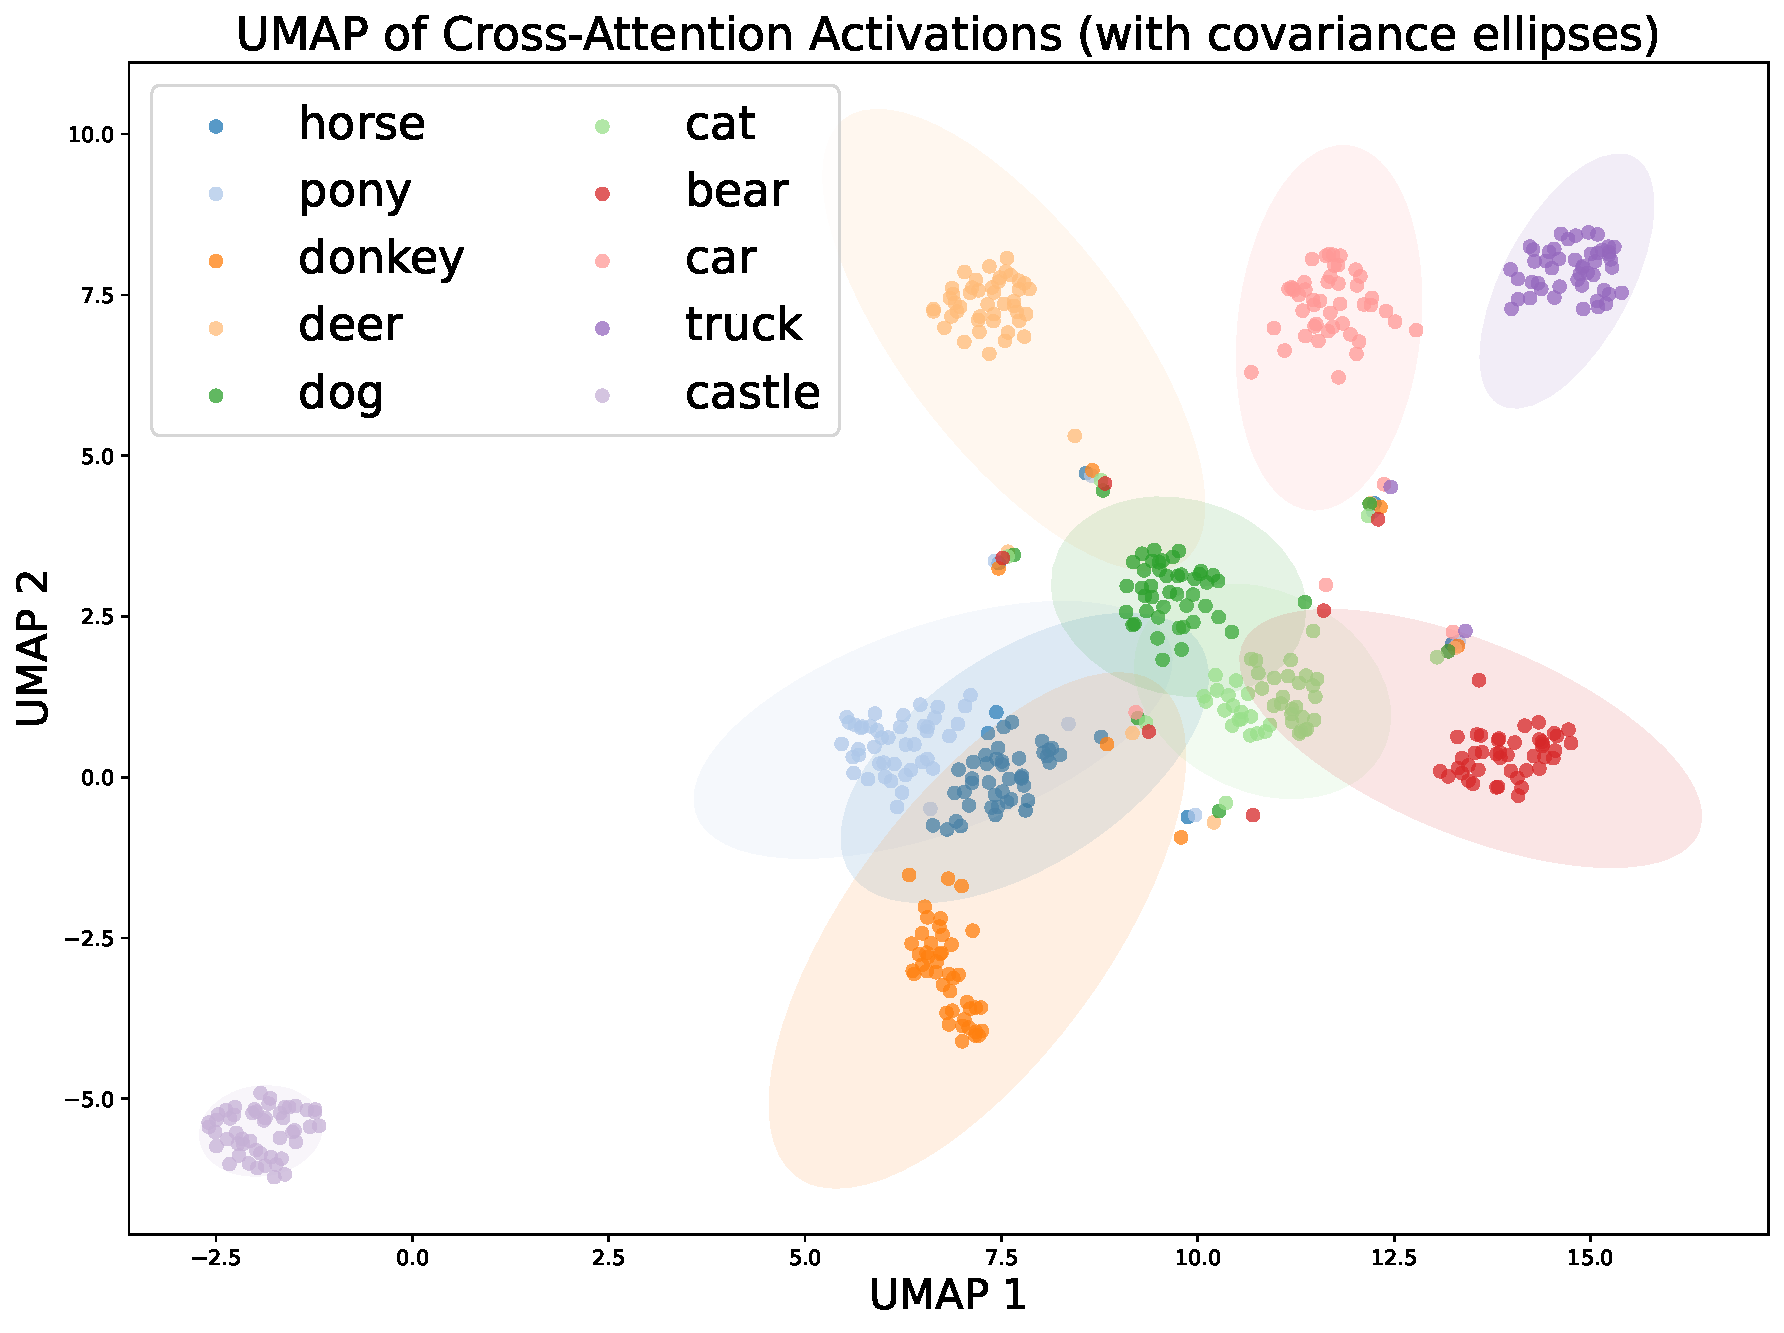
\includegraphics[width=\linewidth]{img/umap_v3_ellipses.pdf}

\vspace{6pt}

\small
\setlength{\tabcolsep}{6pt}
\begin{tabular}{lcl}
\toprule
Concept & $\hat\kappa$ & Neighbors \\
\midrule
dog    & 0.89 & puppy, labrador \\
bear   & 0.82 & black bear, grizzly \\
horse  & 0.81 & donkey, foal, mare \\
cat    & 0.77 & kitten, panther \\
castle & 0.27 & fortress, palace, citadel \\
\bottomrule
\end{tabular}
\end{minipage}\hfill
\begin{minipage}[c]{0.42\linewidth}
\caption{\textbf{Concepts occupy coherent, partially overlapping regions in activation space.}
\emph{Top-left:} UMAP projection of cross-attention activations at \texttt{mid\_block.attentions.0} (step 25/50) for 10 concepts in Stable Diffusion v1.4 (visualization pool; full evaluation pool in~\Cref{app:vocab}); each point is one prompt and ellipses show 95\% covariance contours. Semantically related concepts (\texttt{horse}/\texttt{pony}/\texttt{donkey}) cluster together, while isolated concepts (\texttt{castle}) are well-separated.
\emph{Bottom-left:} Estimated entanglement coefficient $\hat\kappa$ (fraction of the target's activation region shared with semantic neighbors; see~\cref{def:overlap}). The Neighbors column lists representative discovered neighbors; full per-target neighbor sets are reported in~\cref{app:kappa_estimation}. Animal subtypes have high $\hat\kappa$ and dense neighbor sets; \texttt{castle} has low $\hat\kappa$ despite a comparable number of architectural neighbors.}
\label{fig:umap_kappa}
% Aliases preserve existing \cref{fig:umap} and \cref{tab:kappa} references elsewhere in the paper; all three labels resolve to this combined float.
\label{fig:umap}
\label{tab:kappa}
\end{minipage}
\end{figure*}

\paragraph{Contributions.} 
\textbf{(i)} We give a geometric account of concept entanglement, showing that the literature's two failure modes, 
% \varun{earlier, you called this concept leakage; be consistent?}
concept leakage and collateral forgetting, are dual symptoms of overlapping concept regions in cross-attention activation space (quantified by an entanglement coefficient $\hat\kappa$), rather than separate algorithmic shortcomings as treated in prior work~\citep{gandikota2023erasing,zhang2024defensive,srivatsan2025stereo,cywinski2025saeuron}. \textbf{(ii)} Building on this account,
% we prove a method-agnostic lower bound
we derive a geometric lower-bound for concept unlearning under empirically-verified assumptions: any method achieving $\varepsilon$-robust erasure must incur utility preservation error $\gamma \geq \kappa(1-\varepsilon)/L$ (\Cref{thm:tradeoff}), with strict impossibility at $\varepsilon = 0$ whenever $\kappa > 0$ (\Cref{cor:impossibility}); this result reframes unlearning as a Pareto problem rather than a dual-objective one. \textbf{(iii)} We validate the predicted $\kappa$-scaled trade-off across seven methods and five concepts spanning a wide range of $\hat\kappa$ values, using a new Neighbor Preservation metric tied to the activation-level $\gamma$ in our theorem.

% In this work, we argue that the UA/RA coupling observed above is not a shortcoming of individual unlearning algorithms but a structural consequence of how concepts are represented in diffusion models. 
% Our approach proceeds in three steps.
% First, we provide empirical evidence that concepts are represented as distributed patterns across correlated tokens, leading to both \emph{concept leakage}, the target concept reappearing under indirect prompts and \emph{collateral forgetting}, degraded generation of semantically related but distinct concepts (\Cref{sec:trade-off}).
% % \varun{what is this? undefined} (\Cref{sec:trade-off}).
% Second, we formalize this phenomenon by introducing concept activation regions and proving that achieving robust erasure necessarily incurs error in preserving remaining concepts (\Cref{sec:motivation}).
% Third, we empirically validate this trade-off across seven unlearning methods, revealing a Pareto frontier between erasure strength and utility preservation (\Cref{sec:experiment}).

% \varun{i still think we don't need this blurb, and it can be merged with the previous paragraph! will give you space for something downstream}

% We make three contributions. \textbf{(i) Concept entanglement in diffusion models:} we show that visual concepts are distributed across correlated tokens, causing concept leakage and collateral forgetting. \textbf{(ii) A fundamental unlearning--retention trade-off:} we prove that $\varepsilon$-robust concept erasure necessarily incurs non-zero error in preserving neighboring concepts, establishing that perfect unlearning and perfect retention cannot be achieved simultaneously. \textbf{(iii) Empirical characterization:} we benchmark seven unlearning methods and observe a consistent Pareto frontier between erasure strength and neighbor preservation.

 

% \varun{you can compress this full paragraph into 1-2 lines and add it to the previous paragraph, as the caption contains a lot of relevant details}
% To further probe the internal structure underlying these effects,~\cref{fig:umap} visualizes cross-attention activations for multiple concepts in Stable Diffusion. The resulting clusters show that prompts associated with the same concept occupy coherent regions in activation space, while concepts with nearby activation centroids in the extracted cross-attention space from neighboring clusters \ali{the second sentence seems to be incomplete?}. For example, \texttt{horse}, \texttt{pony}, and \texttt{donkey} form a dense equine cluster, while \texttt{castle} is well-separated from all animal concepts. 



% \varun{but who decides these are semantically related? you are making an informed decision; it is not learnt in some unsupervised manner?} 
% \begin{figure}[t]
% \centering
% 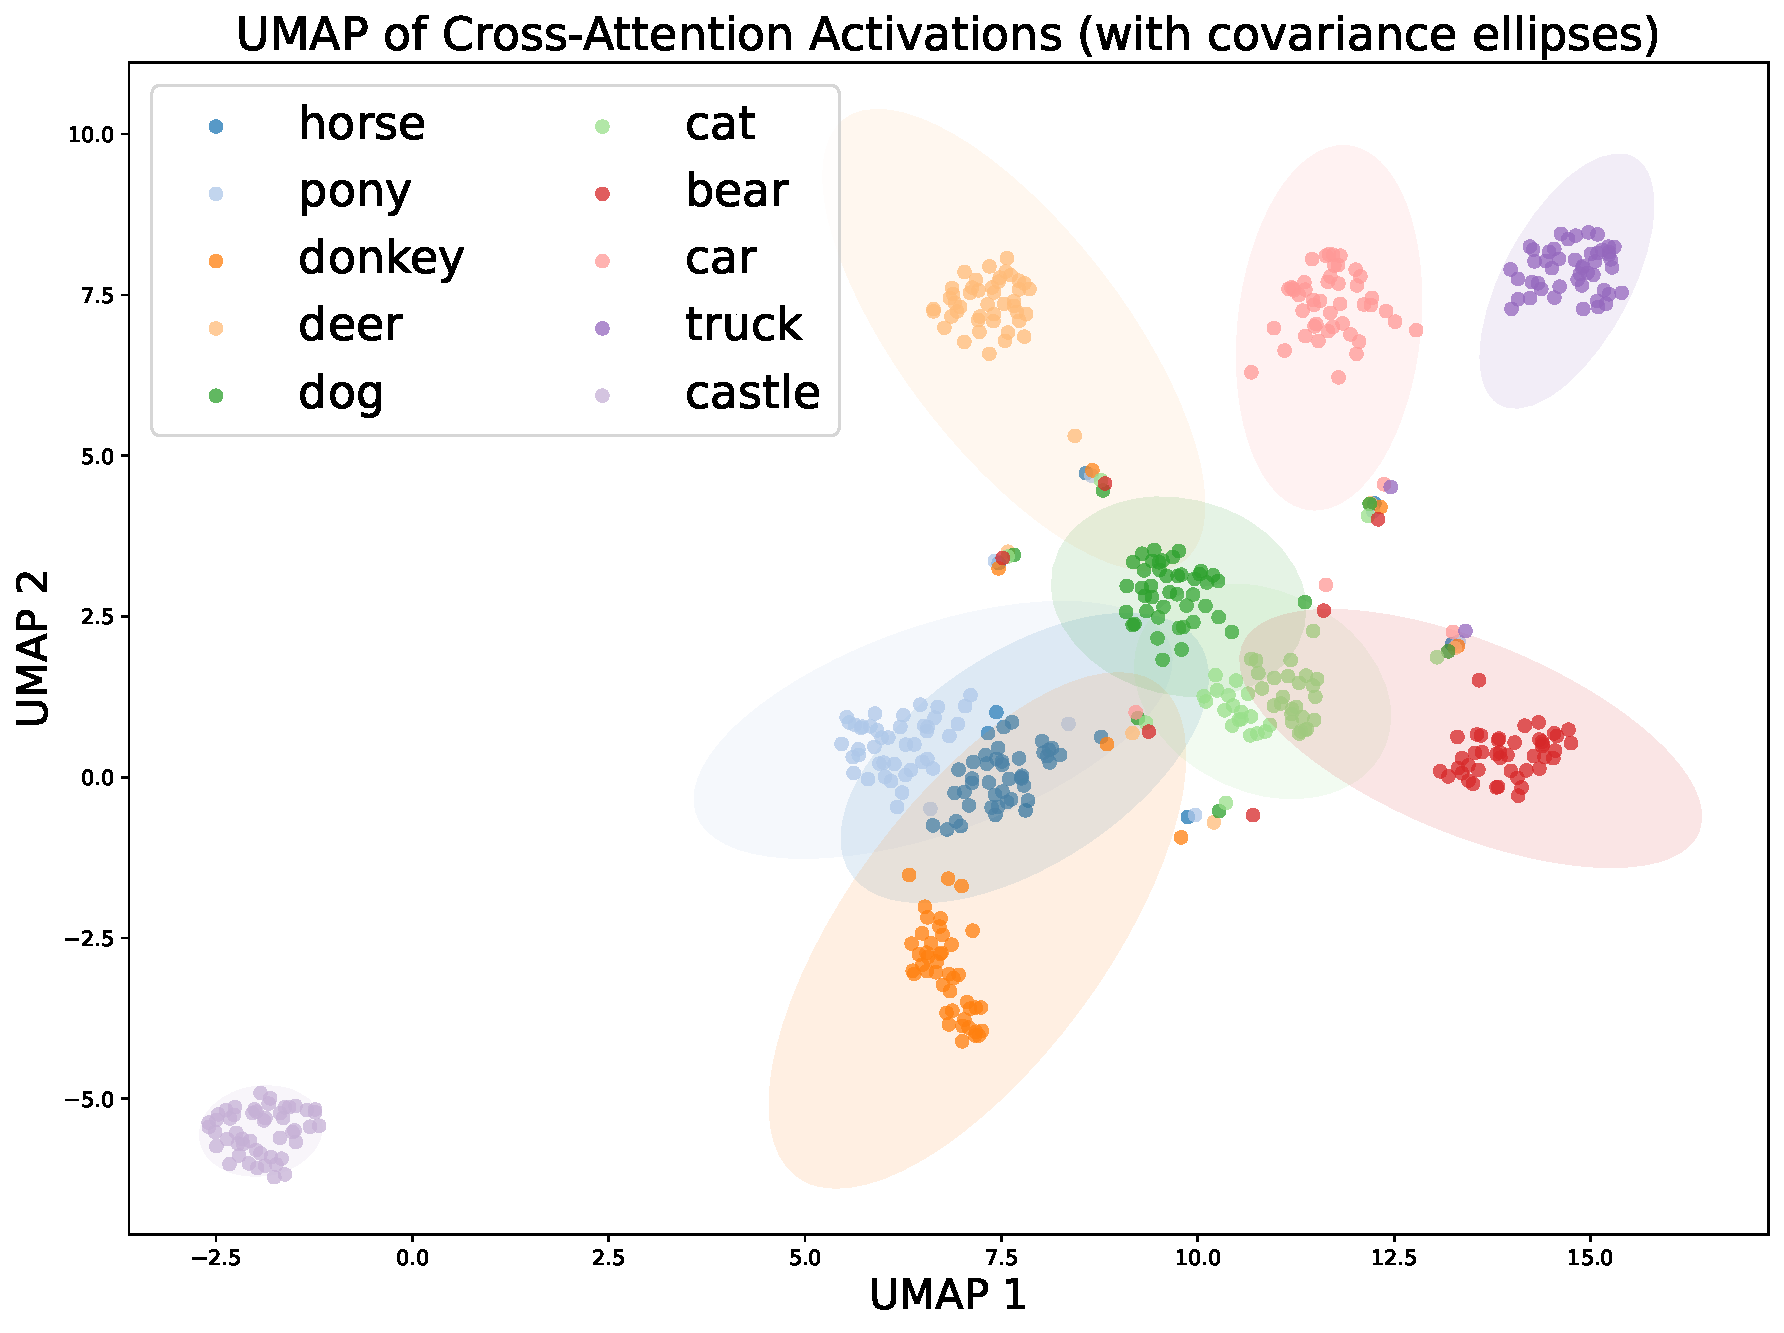
\includegraphics[width=0.6\linewidth]{img/umap_v3_ellipses.pdf}
% \caption{
% UMAP projection of cross-attention activations at \texttt{mid\_block.attentions.0} (step 25/50) for 10 concepts in Stable Diffusion v1.4. Each point corresponds to one prompt; ellipses show 95\% covariance contours. Semantically related concepts (\texttt{horse}/\texttt{pony}/\texttt{donkey}) cluster together, while isolated concepts (\texttt{castle}) are well-separated, confirming that concept activation regions (\Cref{def:activation}) are coherent, localizable structures. 
% % \varun{can make caption scriptsize; can also make the figure a "wrapfig" so that it occupies less space; in that case: please make the legend bigger?}
% % \ali{maybe instead of wrap figure, you can make a single figure side by side with Figure 2 and reduce the size of their captions (captions are too long i think) }
% % \ali{deer in this figure seems to be isolated from horse as well, but in the section for Effect 2, we are claiming that unlearning horse leads to collateral damage on related concepts such as deer. So either the figure needs adjustment or the text and examples.} \yian{I'll adjust the text part in appendix}
% % \varun{+1 for ali's suggestion, but with table 1 instead of fig 2}}
% \label{fig:umap}
% \end{figure}

% \varun{would remove the contributions bullets to save space}
% \paragraph{Contributions.} Our main contributions are:
% \begin{itemize}
% \item \textbf{Concept entanglement in diffusion models.}
% We show that visual concepts are distributed  across correlated tokens, causing concept leakage and collateral forgetting.
% \item \textbf{A fundamental unlearning--retention trade-off.}
% We prove that $\varepsilon$-robust concept erasure necessarily incurs non-zero error in preserving neighboring concepts, establishing that perfect unlearning and perfect retention cannot be achieved simultaneously.
% \item \textbf{Empirical characterization of the trade-off.}
% We benchmark seven unlearning methods and observe a consistent Pareto frontier between erasure strength and neighbor preservation.
% \end{itemize}


\begin{comment}
\varun{which section are these results in?}
First, we provide \textbf{empirical evidence of concept entanglement} in diffusion models (\S\ref{sec:trade-off}). We demonstrate that visual concepts are not represented as isolated, token-aligned features in the model's joint text--image space, but instead emerge from distributed co-occurrence patterns across correlated tokens. This entanglement has two observable consequences that are, in fact, two sides of the same coin: (i) \emph{concept leakage}---an erased concept can be regenerated through semantically related prompts that omit the target token; and (ii) \emph{collateral forgetting}---aggressively suppressing one concept damages the model's ability to generate neighboring concepts whose activation regions overlap with the target. We show both effects empirically across multiple unlearning methods.

\varun{which section are these results in?}
Second, we \textbf{formalize the robustness--retention trade-off} as a provable impossibility result (\S\ref{sec:motivation}). Working in the model's internal activation space, we define concept activation regions, their semantic neighborhoods, and an overlap coefficient $\kappa$ that quantifies the degree of entanglement between a target concept and its neighbors. Under mild continuity assumptions, we prove that any unlearning method achieving $\varepsilon$-robust erasure of a target concept must incur neighbor preservation error of at least $\gamma \geq \kappa \cdot (1-\varepsilon)/L - \delta$ (Theorem~\ref{thm:tradeoff}), where $L$ is a Lipschitz constant and $\delta$ captures the activation-space distance between concepts. A direct corollary establishes that \emph{simultaneous perfect erasure and perfect retention is impossible} whenever the target concept has nonzero overlap with its semantic neighborhood (Corollary~\ref{cor:impossibility}). This result provides a formal explanation for why existing methods are forced to navigate a Pareto frontier rather than achieve ideal performance on both axes.

\varun{which section are these results in?}
Third, we conduct a \textbf{comprehensive empirical study of the trade-off across seven unlearning methods} (\S\ref{sec:experiment}), spanning both fine-tuning-based and inference-time approaches. Using the \textsc{UnlearnCanvas} benchmark~\citep{zhang2024unlearncanvas}, we evaluate each method not only on standard UA, IRA, and CRA metrics but also on a new \emph{neighbor preservation} metric that measures collateral damage on semantically related concepts. Our results reveal a clear Pareto frontier: methods that achieve stronger erasure---particularly those employing adversarial training for robustness---systematically incur greater collateral damage on neighboring concepts, while inference-time methods that preserve neighbors more faithfully tend to leave residual pathways through which erased concepts can be recovered. We further show that the severity of the trade-off is governed by the semantic density of the target concept's neighborhood, consistent with the predictions of our theoretical framework.

\varun{maybe remove this below, as the previous 3 paragraphs are all contributions?}
\paragraph{Contributions.} Our main contributions are:
\begin{enumerate}
    \item \textbf{A formal impossibility result.} We prove that $\varepsilon$-robust concept erasure necessarily incurs neighbor preservation error lower-bounded by the concept overlap coefficient $\kappa$, establishing that the robustness--retention trade-off is a structural property of entangled concept representations, not an artifact of suboptimal algorithm design.
    
    \item \textbf{Empirical Pareto frontier.} We benchmark seven concept unlearning methods on both erasure completeness and neighbor preservation, revealing a consistent trade-off curve and identifying the mechanism-level factors (weight modification scope, intervention granularity) that determine where each method falls on this frontier.
    
    \item \textbf{Unified perspective on concept leakage and collateral forgetting.} We show that these two previously separate failure modes---vulnerability to indirect prompts and degradation of related concepts---are dual consequences of concept entanglement, providing a coherent framework for understanding and evaluating unlearning methods.
\end{enumerate}
\end{comment}

\section{Background \& Related Work}
\label{sec:background}
This section introduces the background on text-to-image diffusion models and reviews existing approaches for concept unlearning in diffusion models.

\subsection{Background}
% \varun{what is the significance of the discussion around diffusion mdoels? why is this primer needed to understand the rest of your paper? need to give that context!}
We briefly introduce the latent diffusion notation used throughout the paper, since our analysis of concept activation regions and unlearning-induced perturbations is defined over the model's latent, text-conditioned denoising process.

\textbf{Text-to-image latent diffusion models.}
We consider a text-to-image latent diffusion model (LDM) of the form introduced in Stable Diffusion~\citep{rombach2022high}.
% We consider a text-to-image latent diffusion model (LDM), following Stable Diffusion~\citep{rombach2022high} \varun{what does it mean to follow?}. 
An input image $\mathbf{x} \in \mathcal{X}$ is first mapped by a pretrained variational autoencoder encoder $E$ into a latent representation 
% \varun{the latent z is bold-faced in the next line, not bold-faced here? subsequent usages are also mixed in usage} 
$\mathbf{z} = E(x) \in \mathcal{Z}$, and reconstructed by a decoder $V : \mathcal{Z} \rightarrow \mathcal{X}$. 

% \ali{I think this is extra info: 
% Instead of modeling pixels directly, the diffusion model operates in latent space, which substantially reduces computation while preserving semantic content.}
Given a latent $\mathbf{z}$, the forward diffusion process corrupts it with Gaussian noise to obtain $\mathbf{z}_t$ at timestep $t \in \{1,\dots,T\}$. 
A time-conditioned U-Net $\boldsymbol{\epsilon}_\theta$ is then trained to predict the noise $\boldsymbol{\epsilon}$ 
% \varun{i would change noise variable to $\eta$ to avoid confuson with the U-net} 
% \yian{kept $\epsilon$/$\epsilon_\theta$ for noise/U-Net to match the standard DDPM convention used in every concept-erasure baseline we compare against (ESD, STEREO, SAeUron, AdvUnlearn).}
added to $\mathbf{z}_t$. 
In text-conditioned generation, a prompt $p \in \mathcal{P}$ is encoded by a text encoder $f_{\psi}$ into text features $\mathbf{e}_p = f_{\psi}(p)$, and these features condition the U-Net through cross-attention layers. 
The standard latent diffusion objective is
\begin{equation}
\label{eq:ldm_loss}
\mathcal{L}_{\mathrm{LDM}}
=
\mathbb{E}_{x,\epsilon,t}
\left[
\left\|
\boldsymbol{\epsilon} - \boldsymbol{\epsilon}_\theta(\mathbf{z}_t, t, \mathbf{e}_p)
\right\|_2^2
\right],
\end{equation}
where $\epsilon \sim \mathcal{N}(0,I)$ 
%\ali{this is redundant: and $z_t$ is the noisy latent corresponding to $z = E(x)$}.
At inference time, generation starts from Gaussian noise and iteratively denoises toward a clean latent, which is finally decoded into an image.

% \ali{maybe "notation" in the name of this section is confusing because most of the notations and definitions will be in section 4.}

% \textbf{Contrast with vision-language models.}
% Although diffusion models use text encoders similar to those used in vision-language models (VLMs)~\citep{radford2021learning}, their training objectives differ fundamentally.
% VLMs such as CLIP are typically trained on large collections of image--text pairs using contrastive objectives that align image and text embeddings by pulling matched pairs together and pushing mismatched pairs apart~\citep{radford2021learning,zhang2024vision}. 
% Thus, VLM training primarily learns \emph{cross-modal alignment} in a shared representation space.
% In contrast, diffusion models use text embeddings as conditioning signals for a denoising generator: the text encoder does not directly predict image-text similarity, but instead provides token-level features that guide image synthesis through cross-attention.
% This distinction matters for unlearning: removing a concept from a generative diffusion model requires changing how text-conditioned denoising gives rise to visual content, not merely altering a retrieval-style similarity score.
% \textbf{Contrast with vision-language models.}
% \ali{I think this section is not necessary as we are not making any comparison or claim regarding the unlearning in VLMs.}
% Both vision-language models (VLMs)~\citep{radford2021learning} and text-to-image diffusion models learn a mapping between textual inputs and visual content. In VLMs, this mapping is used to align images and captions in a shared embedding space, while in diffusion models, text embeddings condition the denoising process that generates images. Thus, in both settings, text representations are tied to visual semantics, but diffusion models use this mapping generatively rather than for retrieval or matching. This distinction is important for unlearning: removing a concept from a diffusion model requires changing how text-conditioned representations give rise to visual content.


%\varun{i think the important part that is not highlighted is how there is text-image mapping in both models; the exact specifics of learning etc. are not relevant and can be removed/moved to appendix?}

% \textbf{Diffusion unlearning.}
% Let $\mathcal{D}_\theta$ denote a pretrained text-to-image diffusion model with parameters $\theta$, and let $c$ denote a target concept to be erased (e.g., \texttt{horse}).
% Diffusion unlearning seeks to produce an updated model $\mathcal{D}_{\theta'}$ such that prompts referring to $c$ no longer generate images containing that concept, while the model retains its ability to generate unrelated content.
% Formally, given a prompt distribution $\mathcal{P}_c$ associated with concept $c$, the goal is to reduce the probability that samples from $\mathcal{D}_{\theta'}(\cdot \mid p)$ contain $c$ for $p \sim \mathcal{P}_c$, while preserving generation quality and fidelity on prompts outside this target concept class. \varun{is there prior work on this? add some pointers, or maybe say this is discussed in intro? maybe this should be merged with the next subsection?}

\subsection{Unlearning Methods}
Machine unlearning in diffusion models aims to remove a target concept $c$ (e.g., \textit{horse}) from a pretrained model $\mathcal{D}_\theta$(the full text-to-image pipeline parameterized by the U-Net weights $\theta$ from Eq.~\ref{eq:ldm_loss}) 
% \varun{use a different variable for params, as the params $\theta$ are used for the U-Net?} 
% \yian{$\theta$ is shared with $\epsilon_\theta$ on purpose as the U-Net is the only trainable component, so $\mathcal{D}_\theta$ and $\epsilon_\theta$ must share parameters. }
while preserving overall generative capabilities. The goal is an updated model $\mathcal{D}_{\hat{\theta}}$ that suppresses $c$ on target-associated prompts while maintaining quality on unrelated prompts, following prior work on concept erasure in diffusion models. 

\textbf{Fine-tuning methods.}
A large body of work erase concepts by directly modifying the weights of a pretrained diffusion model. Erased Stable Diffusion (ESD)~\cite{gandikota2023erasing} uses negative guidance to align target-token prompts with a neutral anchor. Subsequent work improves the precision by editing cross-attention representations~\citep{wang2025ace} or updating salient concept-related parameters~\citep{fan2023salun,wu2024scissorhands}. More recent robust methods such as AdvUnlearn~\cite{zhang2024defensive} and STEREO~\cite{srivatsan2025stereo} further defend against prompt-based regeneration attacks.
However, these methods still largely define erasure through target tokens, prompts, or localized parameter subsets. They therefore suppress direct target prompts well, but struggle with \emph{concept leakage} through correlated context; when made more aggressive, their edits can propagate through shared representations and cause \emph{collateral damage} to semantic neighbors.

\textbf{Inference-time methods.}
A complementary line of work avoids modifying $\mathcal{D}_{\theta}$ and instead intervenes during generation by manipulating text embeddings~\citep{li2024get}, inserting lightweight concept-blocking adapters~\citep{lyu2024one}, or ablating sparse-autoencoder features~\citep{cywinski2025saeuron}. These methods are computationally efficient and often preserve broad model behavior, but their conservative, localized interventions do not remove the distributed contextual pathways through which a target concept can be recovered. As a result, they tend to preserve neighboring concepts better, while leaving residual indirect recovery.

\noindent{\bf Shared limitation.}
Thus, both fine-tuning and inference-time methods implicitly treat concepts as localized and independently suppressible. Our work challenges this assumption: when concepts occupy overlapping activation regions, erasure and retention are coupled, so stronger robustness against leakage necessarily increases the risk of neighbor degradation.

%\ali{we should somehow highlight this last paragraph; readers usually skip the related work sections.}
% \noindent\textbf{Takeaway.}
% Existing unlearning algorithms operate under the assumption that concepts can be selectively removed from the model’s representation space. In the following section, we provide empirical evidence that challenges this assumption by demonstrating that concepts remain recoverable through correlated contextual prompts.
% \noindent \textbf{Data Unlearning}
% \cite{alberti2025data}

\begin{comment}
    \subsection{Unlearning Methods}
% \noindent \textbf{The \textsc{UnlearnCanvas} Benchmark}
% Our experimental framework is built upon the \textsc{UnlearnCanvas} benchmark, a comprehensive dataset recently proposed by~\citet{zhang2024unlearncanvas} to standardize the evaluation of diffusion model unlearning. It was created to address the lack of rigorous, automated evaluation frameworks, which previously relied on ad-hoc, qualitative assessments. The benchmark consists of a high-resolution, stylized image dataset featuring 65 distinct artistic styles and 20 distinct object classes. Its primary advantage lies in its high stylistic consistency, which enables the training of a highly accurate style classifier, allowing for the reliable, quantitative measurement of unlearning using standardized metrics like Unlearning Accuracy (UA), In-domain Retain Accuracy (IRA), and Cross-domain Retain Accuracy (CRA). While \textsc{UnlearnCanvas} provides the essential visual data for our investigation, it does not include a formal, art style hierarchy linking its 60 styles. The styles are presented as a flat list. A foundational part of our methodology, therefore, is to construct this missing knowledge graph, which serves as the basis for our directional unlearning experiments.

\noindent \textbf{Methods for Diffusion Model Unlearning}
The primary objective of Machine Unlearning (MU) in diffusion models is to erase a target concept while minimizing collateral damage to the model's remaining generative capabilities. Current approaches can be broadly classified into two main categories:

\textbf{1. Fine-Tuning Methods:} This line of work involves permanently altering the model's weights. Many of these methods, such as Erased Stable Diffusion (ESD)~\cite{gandikota2023erasing}, utilize a form of negative guidance, retraining the model to align the output of the "forget" prompt with that of a neutral anchor prompt. Variations of this approach aim for greater precision. 
For example,~\citet{zhang2024forget} applies a re-steering loss to attention layers, while~\citet{fan2023salun} and~\citet{wu2024scissorhands} identify and modify only the most sensitive weights. 
\cite{zhang2024defensive} propose \textit{AdvUnlearn}, which integrates adversarial training into diffusion model unlearning to improve robustness against prompt-based attacks that attempt to regenerate erased concepts.
Attention-based Concept Erasure (ACE)~\cite{wang2025ace} removes target concepts by modifying cross-attention representations associated with the concept tokens, enabling localized editing of concept-related activations within the diffusion model.
STEREO~\cite{srivatsan2025stereo} introduces a robust concept unlearning framework that enforces separation between target and neighboring concepts, improving resistance to prompt-based regeneration of erased concepts.
%More recently,~\citet{li2025set} proposes a trajectory-aware finetuning framework that explicitly preserves early-stage denoising dynamics while reversing classifier-free guidance directions during mid-to-late stages, enabling precise concept erasure without relying on heuristic anchor selection.

Other notable fine-tuning methods include Unified Concept Editing (UCE)~\cite{gandikota2024unified}, Concept Ablation~\cite{vinker2023concept}, Selective Amnesia (SA)~\cite{heng2023selective}, and EraseDiff (EDiff)~\cite{wu2024erasediff}. 

While effective, these methods are vulnerable to "jailbreak" attacks that exploit related concepts~\cite{zhang2024generate} and operationally treat concepts as isolated entities. Orthogonal to concept-level unlearning,~\citet{alberti2025data} formalize datapoint-level unlearning in diffusion models and introduce Subtracted Importance Sampled Scores (SISS), an efficient fine-tuning objective with theoretical guarantees that aims to match the retrain-without-data gold standard at far lower cost~\cite{alberti2025data}

\textbf{2. Inference-Time Methods:} A second class of methods avoids the costly fine-tuning step by intervening directly during the generation process, leaving the model's original weights untouched. These techniques are often more efficient and can be dynamically toggled. SEOT~\cite{li2024get}suppresses unwanted content by manipulating text embeddings, and SPM~\cite{lyu2024one} uses lightweight one-dimensional adapters to block the propagation of concept-specific information. A highly relevant new approach in this category is SAeUron~\cite{cywinski2025saeuron}. This method leverages Sparse Autoencoders (SAEs) trained on the model's internal activations to learn a dictionary of sparse, interpretable features.And unlearning is achieved at inference time by identifying the features that correspond to an unwanted concept and ablating them, preventing their contribution to the final image. While these methods also treat concepts in isolation, their interventional nature inspires our work. We leverage similar interventions not just for deletion, but as a method to discover the latent structure of conceptual relationships. 
\end{comment}
%\section{The Unlearn--Retain Tension}
\section{Motivation}
\label{sec:motivation} 
Current concept unlearning methods are designed to suppress a concept token (e.g., ``\texttt{horse}'') 
% \varun{you used \texttt{horse} earlier; be consistent?} 
so as to remove the corresponding visual concept without substantially affecting other concepts. This design implicitly assumes that visual concepts are represented as localized, token-aligned features in the model's joint text--image space.
In this section, we present empirical evidence that this assumption fails: 
in practice, unlearning a target concept produces 
% \emph{collateral damage} to semantically neighboring concepts 
\emph{collateral damage} to the concepts with which it is entangled. 
% \footnote{We define semantic neighborhood formally in \cref{subsec:definitions} as the set of concepts whose activation regions in the model's cross-attention space lie within distance $\delta$ of the target's. In this section, ``neighbors'' refers operationally to fine-grained subtypes and near-synonyms (e.g., \texttt{donkey}, \texttt{pony} for \texttt{horse}).}
\footnote{We define entanglement formally in \cref{subsec:definitions} based on activation regions in the model's cross-attention space.}
%, and the severity of that damage is coupled to the robustness \footnote{Throughout this section, ``robustness'' refers informally to how reliably the target concept is suppressed across diverse prompts, including indirect ones that do not mention the concept word. We make this precise as $\varepsilon$-robust unlearning in \cref{def:robust}.} of the erasure. 
The severity of this damage is coupled to both the strength of the erasure applied to the target concept and the extent of its entanglement with other concepts.
This coupling is the phenomenon our theoretical framework analyzes in~\cref{sec:tradeoff}.

% diffusion models exhibit strong \emph{concept entanglement}, where semantically related concepts share overlapping representational structure. 
% This entanglement produces two observable consequences---concept leakage and collateral forgetting---that we argue are not independent failure modes but rather \emph{dual manifestations of the same underlying phenomenon}: shared representational structure across correlated concepts.

% Two observations drive this framing. First, diffusion models condition on prompt embeddings produced by text encoders that exhibit bag-of-words behavior~\citep{yuksekgonul2022and}: prompts that omit a concept token (\emph{horse}) but retain its typical context (\emph{jockey}, \emph{saddle}, \emph{racetrack}) can still induce activations associated with that concept. \varun{thus?} The visual concept is distributed across ``correlated'' context tokens, not isolated in a single word. \varun{examples? point to fig?}
%Second, semantically neighboring concepts share much of this context (\emph{``a horse in a field''}, \emph{``a donkey in a field''}), causing their activation regions to overlap \varun{so what?}. Together these observations imply that any intervention modifying the activation region of one concept will propagate to its neighbors.

The training mechanisms of text-to-image diffusion models make entanglement inevitable.
First, diffusion models condition on prompt embeddings produced by text encoders that often exhibit bag-of-words behavior~\citep{yuksekgonul2022and}. As a result, prompts that omit a concept token (e.g., \texttt{horse}) but retain its characteristic context (e.g., \texttt{jockey}, \texttt{saddle}, \texttt{racetrack})
% \varun{again, use texttt?}
can still induce activations associated with that concept (see~\cref{fig:bow_context_span}). This implies that the visual concept is not localized in a single token, but is instead distributed across multiple correlated context tokens. Second, semantically related concepts share much of this contextual structure (e.g., \emph{a horse in a field''} vs.\ \emph{a donkey in a field''}), which leads to overlapping activation regions in the model’s internal representation space.

\Cref{fig:concept_leakage} illustrates an example of the trade-off due to this entanglement. It shows two unlearning methods using \texttt{horse} as the erasure target.
% \ali{the figure does not seem to match the description here anymore?}.
Method that perform localized erasure (ESD~\cite{gandikota2023erasing}) successfully suppress generation when the target token is named, but regenerate the concept through indirect prompts that name only context words, which we call \emph{concept leakage}. 
Methods that erase more aggressively (STEREO~\cite{srivatsan2025stereo}) suppress this leakage but produce visibly degraded outputs for some semantically similar concepts, such as \texttt{donkey} and \texttt{zebra}, that are entangled with the target concept (see~\cref{tab:kappa}). We call this effect \emph{collateral damage}. 

Together, these observations imply that modifying the activation region of a target concept necessarily affects other concepts that rely on the same shared representation. In other words, interventions intended to suppress a concept will propagate to concepts with which is it entangled, giving rise to both concept leakage and collateral damage. 
%\varun{i would comment the rest of this text} In~\cref{sec:tradeoff} we formalize this constraint as a provable lower bound on the trade-off between erasure effectiveness and utility preservation. And in~\cref{sec:experiment}, we validate the trade-off quantitatively across seven unlearning methods.

\begin{comment}
    \subsection{Why Concepts Are Entangled: Distributed Representations in Diffusion Models}
\label{subsec:bow}

The roots of concept entanglement lie in how diffusion models process text. These models condition image generation on embeddings produced by pretrained text encoders (e.g., CLIP~\citep{radford2021learning}), which have been shown to exhibit \emph{bag-of-words} behavior: prompt embeddings are often well-approximated by aggregations over individual token embeddings, with limited sensitivity to word order and relational bindings~\citep{yuksekgonul2022and}.
Following this observation, we view the prompt embedding $f_\psi(p)$ as being influenced not only by the token naming a concept, but also by the surrounding context tokens that frequently co-occur with it.
% Under such a representation, if the text encoder behaves approximately as
% \begin{equation}
%     f_\psi(p) \;\approx\; \sum_{t \in p} \boldsymbol{\Phi}(t),
% \end{equation}
% where $\mathrm{Tok}(p)$ denotes the tokens in prompt $p$ \varun{where is $\mathrm{Tok}(p)$ used? should it be $t \in Tok(p)$?}, and $\boldsymbol{\Phi}(t)$ is the embedding of token $t$ \varun{why a different embedding function and not $f_\psi$?},
% then the embedding of a concept is not determined by a single token but by the \emph{constellation of co-occurring tokens} in its typical prompt context \varun{what does constellation mean in this context? also, is the equation above from yuksekgonul's paper? if so -- state it! if not, provide more justification for why it is a sum?}. 
For example, prompts involving the concept \texttt{horse} often contain context words such as \emph{rider}, \emph{saddle}, \emph{barn}, or \emph{galloping}. As a result, the model can associate the visual concept with a broader textual context rather than with a single lexical item alone.
% Training captions in large-scale text-to-image datasets reinforce this: captions containing the concept \texttt{horse} frequently include tokens such as \emph{rider}, \emph{saddle}, \emph{cowboy}, and \emph{stable} \varun{so what?}. 
For simplicity, let $t_c$ denote the token %\varun{what if horse is split into 2 tokens? state that you're making a simplifying assumption that the concept corresponds to a single token} 
corresponding to concept $c$, 
and let $S_c$ denote a set of context tokens that frequently co-occur with $t_c$ in prompts. 
Then prompts that omit $t_c$ but retain enough of $S_c$ can still produce text embeddings similar to those of prompts that explicitly contain $t_c$. At a high level, this suggests that
\begin{equation}
\label{eq:bow_approx}
\mathbb{E}[\mathbf{e}_p \mid t_c \in p]
\;\approx\;
\mathbb{E}[\mathbf{e}_p \mid S_c \subseteq p].
\end{equation}
where $\mathbf{e}_p = f_\psi(p)$ denotes the prompt embedding.

% \ali{is $\mathbf{e}_p$ same as $e_p$ in the definitions. make sure notations is consistent.}
\varun{i don't understand the equation above? it is saying that in expectation, the embeddings are the same? but maybe the RHS needs to be more specific to say that $t_c \notin p$? otherwise it is not communicating the point you want to make}

\ali{i think it might be better to use an equation that implies the image generation on the prompts from $S_c$ is almost the same. claiming that prompt embeddings are the same is not what we directly evaluate? maybe something like this:
\[
\mathbb{E}_{p \sim \mathcal{P}(t_c)} \left[\, 
\Pr_{x \sim p_\theta(\cdot \mid p)}\big[O_X(x, c) = 1\big] 
\,\right]
\;\approx\;
\mathbb{E}_{p \sim \mathcal{P}(S_c \setminus t_c)} \left[\, 
\Pr_{x \sim p_\theta(\cdot \mid p)}\big[O_X(x, c) = 1\big] 
\,\right]
\]
}

This means that the representation of concept $c$ is distributed across correlated context tokens, not isolated in a single word. 
The same logic also explains why neighboring concepts can overlap. For instance, prompts such as a horse in a field,'' a deer in a field,'' and ``a zebra in a field'' share a common contextual scaffold while differing in only one concept token.
% Crucially, neighboring concepts (e.g., \texttt{deer}, \texttt{zebra}) share many of the same contextual tokens (e.g., \emph{field}, \emph{galloping}, \emph{animal}), causing their activation regions in the model's internal representation space to overlap. 
% \varun{this is not coming across from the theory or the equations above! you may want to show that there are many prompts of a "fixed" structure where only one token varies. for example: in the farm, there is a "cow/horse/dog" etc -- and this can motivate what neighboring concepts are.} 
Because these prompts induce similar text-conditioned activations, the corresponding concepts can have overlapping regions in the model's internal representation space.
This overlap creates the fundamental tension we study: suppressing one concept by modifying the shared region can also disturb neighboring concepts that rely on the same contextual structure.%any intervention that modifies the shared representational region to suppress one concept risks disrupting its neighbors. \varun{equation 3 and 2 do not show that, so this last statement is not motivated thus far!}

\end{comment}

%\paragraph{Two Sides of the Same Coin}
% We now demonstrate that concept entanglement produces two empirically observable effects that constrain every unlearning method. These effects are not independent failure modes to be addressed separately; they are coupled consequences of representational overlap. 

%\ali{I think the section starts very abruptly with Figure 2 illustrates "the consequence" of "this" structure. what consequence? what structure? the section should be kind of self-contained. So I think either remove the hearder and merge with the previous text or add a couple of sentences at the begenning. }

%\Cref{fig:concept_leakage} illustrates the consequence of this structure using \texttt{horse} as the erasure target across two unlearning methods.
% \ali{the figure does not seem to match the description here anymore?}.
%Method that perform localized erasure (ESD~\cite{gandikota2023erasing}) successfully suppress generation when the target token is named, but regenerate the concept through indirect prompts that name only context words, which we call \emph{concept leakage}. 
%Methods that erase more aggressively (STEREO~\cite{srivatsan2025stereo}) suppress this leakage but produce visibly degraded outputs for semantically neighboring concepts such as \texttt{donkey} and \texttt{zebra} after erasing \texttt{horse}, which we consider \emph{collateral damage to neighbors}. 
% No method in our study simultaneously avoids both failures.

% \paragraph{Effect 1: Concept leakage through correlated prompts.}
% After applying each unlearning method to erase \texttt{horse}, we test whether the concept can be regenerated using prompts that omit the target token but include semantically related context. Example prompts include \emph{``Image of the animal a jockey rides at the racetrack''} and \emph{``A royal procession with decorated ceremonial mounts.''}

% As shown in Figure~\ref{fig:concept_leakage}, methods that perform lightweight or localized erasure (ESD, SAeUron) successfully suppress the concept when the token \texttt{horse} appears in the prompt, but still regenerate it for a substantial fraction of contextual prompts that omit the target token.
% \yian{Concretely, over (N) indirect prompts, ESD regenerates horse-like images in () cases, and SAeUron does so in () cases.}
% \varun{more precise? how many tries, how many successes etc.?}. 
% This is a direct consequence of Eq.~\eqref{eq:bow_approx}: the model's representation of \texttt{horse} extends beyond the token itself into a broader region of activation space populated by co-occurring tokens. Unlearning the token's direct contribution leaves this broader region largely intact.

% \paragraph{Effect 2: Collateral forgetting of neighboring concepts.}
% Methods that achieve more aggressive erasure---particularly STEREO, which uses a form of adversarial training to suppress the concept across a wide region of embedding space---substantially reduce concept leakage. However, this robustness comes at a cost. After erasing \texttt{horse} with STEREO, we observe significant degradation in the model's ability to generate semantically neighboring concepts. Prompts such as \emph{``a deer standing in a forest''} and \emph{``a herd of deer grazing in a field''} produce distorted or incorrect outputs.

% TODO: Add a figure here showing neighbor degradation (deer/zebra/giraffe generation 
% quality before and after horse erasure, across methods). This is the most impactful 
% figure for the trade-off story.

% This collateral damage is consistent with the overlap pattern in~\cref{fig:umap}.
% In particular, prompts that share the same contextual scaffold but differ only in the concept token induce nearby cross-attention activations.\varun{proof? this is what i wanted to see in an earlier comment}. This suggests that corresponding concepts occupy overlapping activation regions, so suppressing the \texttt{horse}-associated region can also perturb neighboring concepts like \texttt{deer}.

% \paragraph{The trade-off.}
% These two effects are inversely related across the methods we examine. ESD and SAeUron preserve neighboring concepts well (low collateral forgetting) but are vulnerable to indirect prompts (high concept leakage). STEREO achieves robust erasure with minimal leakage but incurs substantial 
% %\varun{you mean collateral? be consistent with terms} 
% collateral damage. This pattern is not coincidental---it reflects a structural constraint imposed by concept entanglement:
% \begin{center}
% \emph{To suppress an entangled concept robustly, a method must modify the shared representational region;\\but modifying the shared region necessarily affects neighboring concepts.}
% \end{center}

% \ali{do we want to blame the concept entanglement directly or blame the way the diffusion models are trained (multi-object images with non-specific captions)?} \varun{training leads to entanglement -- this is the story?}
% \yian{it could be }
%\yian{This limitation is not specific to any particular unlearning method, just arises from how diffusion models are trained? Large-scale text-to-image datasets contain multi-object scenes with weakly structured captions, so semantically related concepts share overlapping activation regions.}

%This inverse relationship is not incidental: it reflects a structural constraint. Robust erasure of an entangled \varun{entanglement not defined} concept requires modifying the shared activation region; but modifying the shared region necessarily disturbs neighboring concepts that depend on it. In~\cref{sec:tradeoff} we formalize this constraint as a provable lower bound on the trade-off between erasure robustness and neighbor preservation. And in~\cref{sec:experiment}, we validate the trade-off quantitatively across seven unlearning methods.

\begin{figure*}[htbp]
\centering
\begin{minipage}[c]{0.5\linewidth}
\centering
\setlength{\tabcolsep}{4pt}
\renewcommand{\arraystretch}{0.9}
\begin{tabular}{c c c c}
 & \textbf{Direct} & \textbf{Indirect} & \textbf{Neighbor} \\
\midrule
\textbf{ESD} &
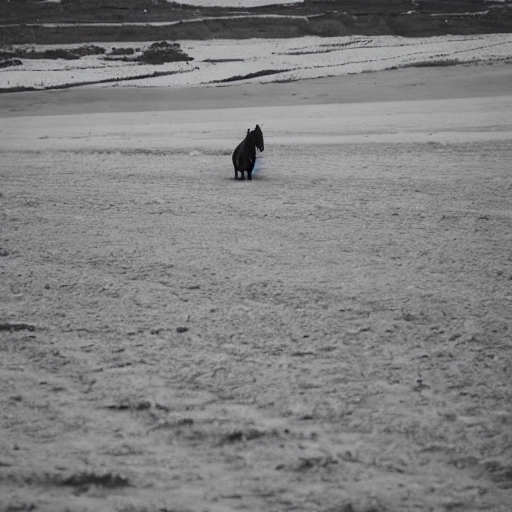
\includegraphics[width=0.28\linewidth]{img/esd_unlearn_horse.png} &
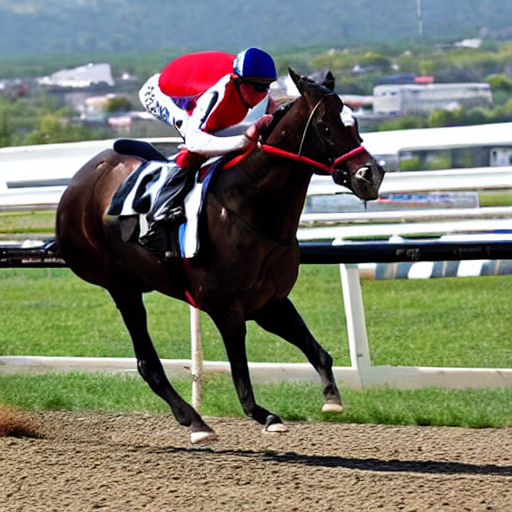
\includegraphics[width=0.28\linewidth]{img/esd_unlearn_nohorse.png} &
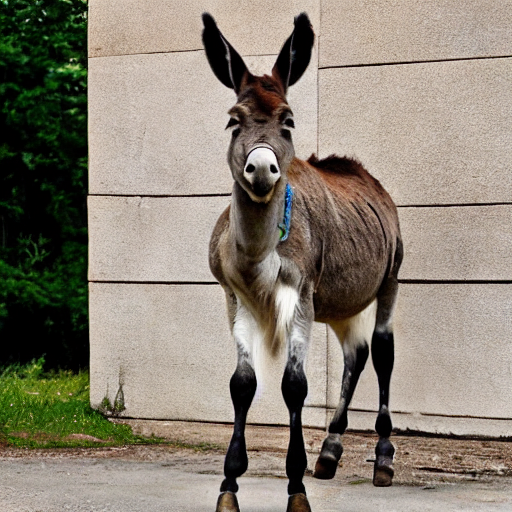
\includegraphics[width=0.28\linewidth]{img/esd_unlearn_donkey.png} \\
\textbf{STEREO} &
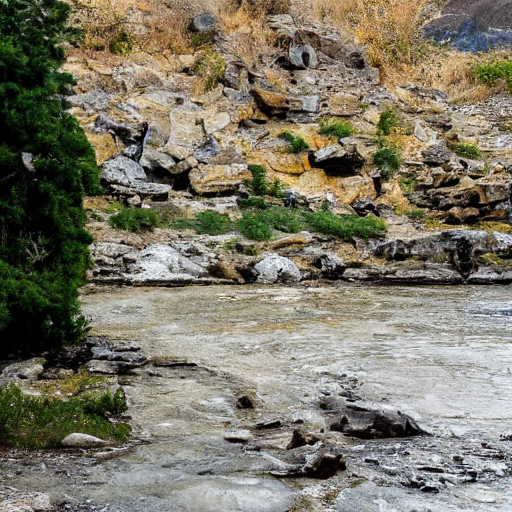
\includegraphics[width=0.28\linewidth]{img/stereo_unlearn_horse.png} &
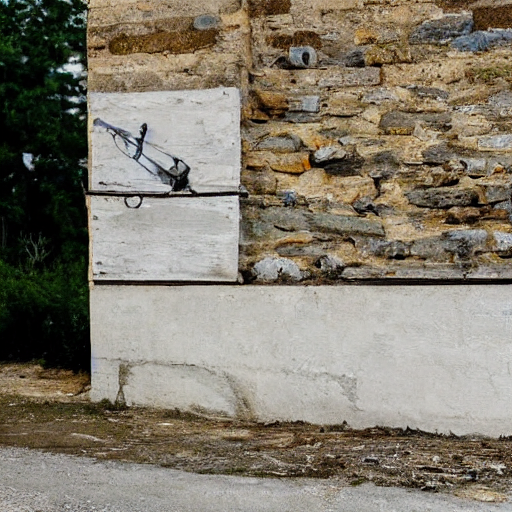
\includegraphics[width=0.28\linewidth]{img/stereo_unlearnnohorse.png} &
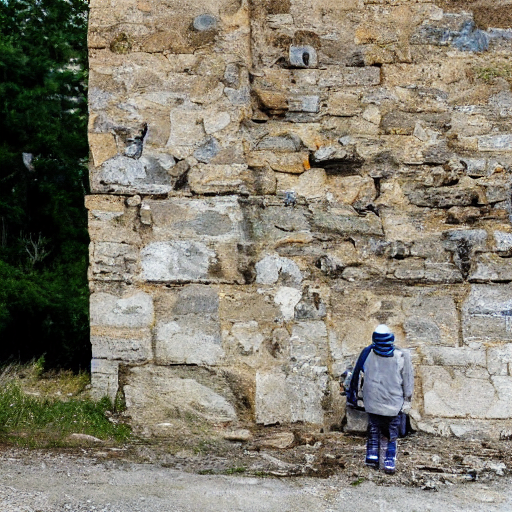
\includegraphics[width=0.28\linewidth]{img/stereo_unlearn_donkey.png} \\
\end{tabular}
\end{minipage}%
\hfill
\begin{minipage}[c]{0.38\linewidth}
\caption{
\textbf{Concept entanglement manifests as two coupled effects.}
Each row erases {horse} and is probed with three prompt types: \emph{Direct} (mentions ``\texttt{horse}''), \emph{Indirect} (uses correlated context like \texttt{jockey} but omits ``\texttt{horse}''), and \texttt{Neighbor} (semantically similar concept \texttt{donkey}). ESD leaks horses through indirect prompts but preserves donkey; STEREO suppresses leakage but destroys donkey. We formalize this duality in~\cref{sec:tradeoff}.
}
\label{fig:concept_leakage}
\end{minipage}
\end{figure*}

% \begin{figure*}[htbp]
% \centering
% \setlength{\tabcolsep}{4pt}
% \renewcommand{\arraystretch}{0.8}
% \begin{tabular}{c c c c}
%  % & \textbf{Prompt with ``horse''} & \textbf{Prompt without ``horse''} & \textbf{Prompt with ``donkey''} \\
%  & \textbf{Direct} & \textbf{Indirect} & \textbf{Neighbor} \\
% \midrule
% \textbf{ESD} &
% 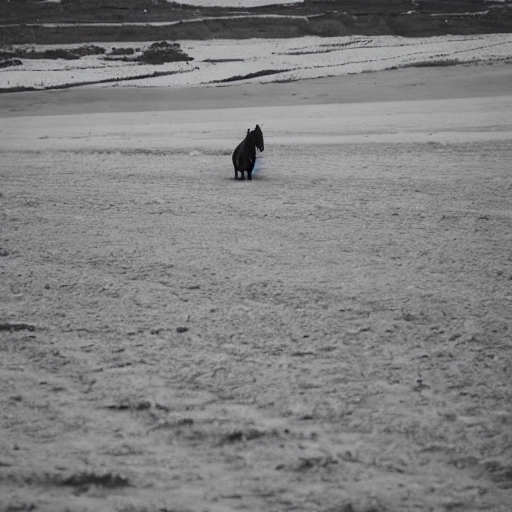
\includegraphics[width=0.15\linewidth]{img/esd_unlearn_horse.png} &
% 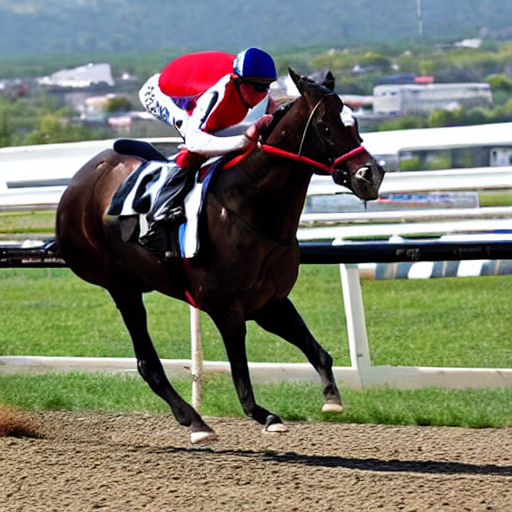
\includegraphics[width=0.15\linewidth]{img/esd_unlearn_nohorse.png} &
% 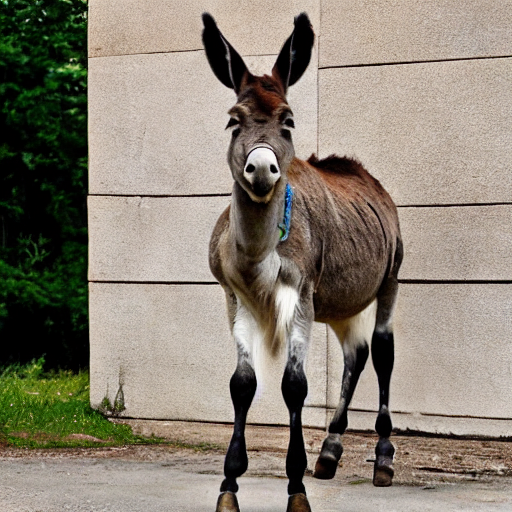
\includegraphics[width=0.15\linewidth]{img/esd_unlearn_donkey.png} \\
% % \textbf{AdvUnlearn} &
% % 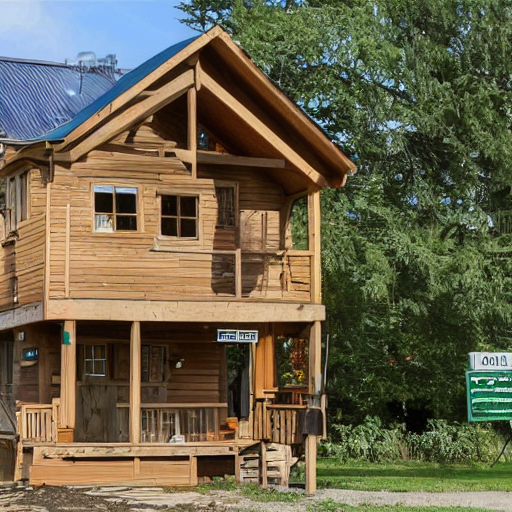
\includegraphics[width=0.13\linewidth]{img/adv_unlearn_horse.png} &
% % 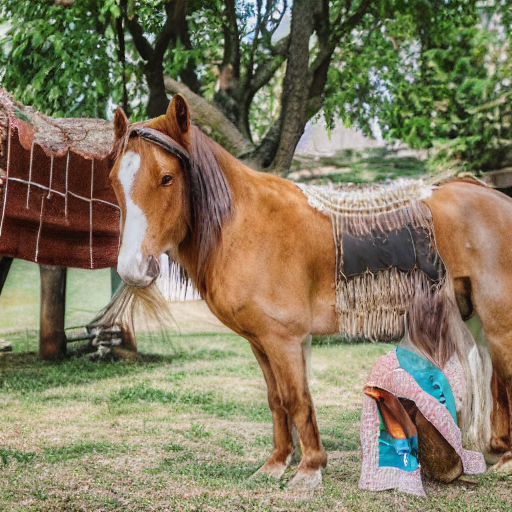
\includegraphics[width=0.13\linewidth]{img/adv_unlearn_nohorse.png} &
% % 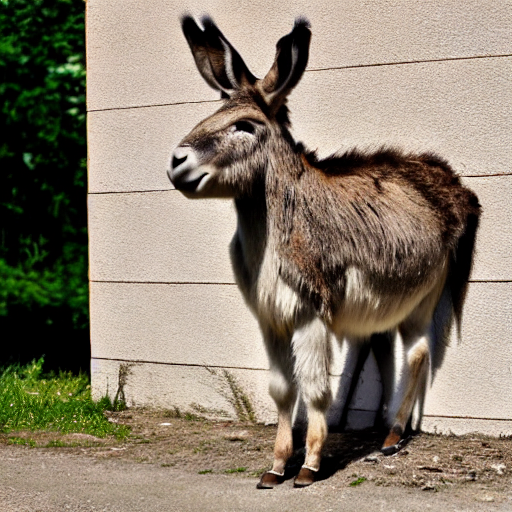
\includegraphics[width=0.13\linewidth]{img/advunlearn_unlearn_donkey.png} \\
% \textbf{STEREO} &
% 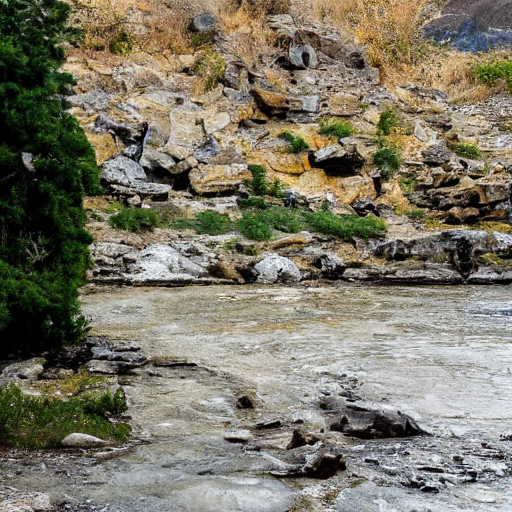
\includegraphics[width=0.15\linewidth]{img/stereo_unlearn_horse.png} &
% 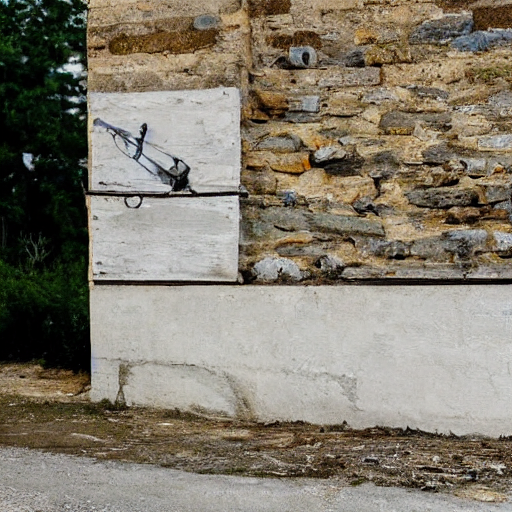
\includegraphics[width=0.15\linewidth]{img/stereo_unlearnnohorse.png} &
% 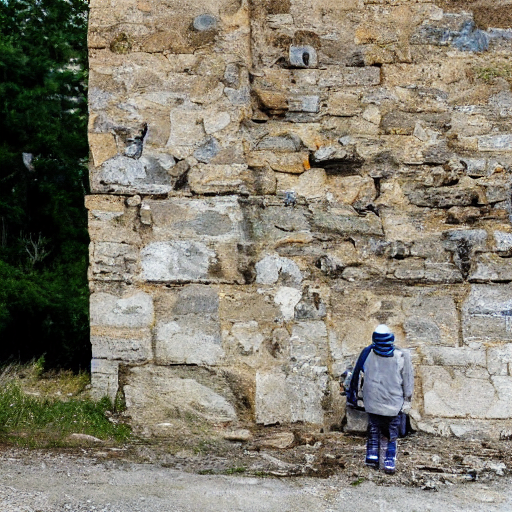
\includegraphics[width=0.15\linewidth]{img/stereo_unlearn_donkey.png} \\
% % \textbf{SAeUron} &
% % 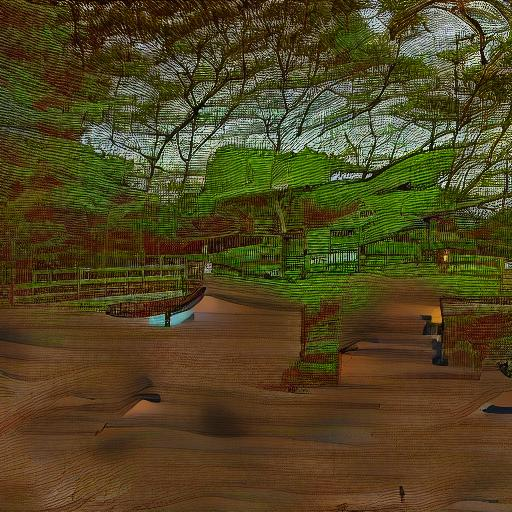
\includegraphics[width=0.13\linewidth]{img/saeuron_unlearn_horse.jpg} &
% % 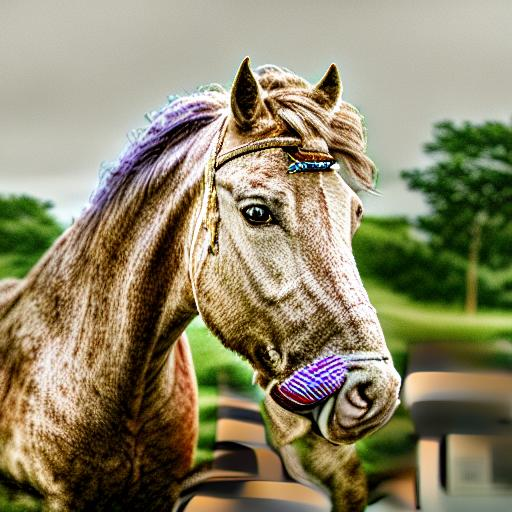
\includegraphics[width=0.13\linewidth]{img/saeuron_unlearn_nohorse.jpg} &
% % 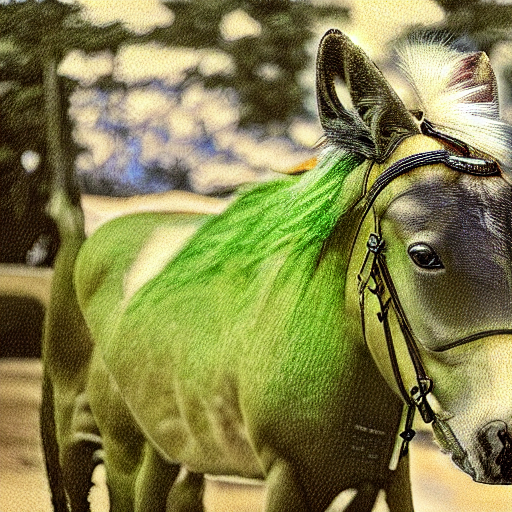
\includegraphics[width=0.13\linewidth]{img/saeuron_unlearn_donkey.png} \\
% \end{tabular}
% \caption{
% \textbf{Concept entanglement manifests as two coupled effects.}
% Each row shows the output of an unlearning method applied to erase \texttt{horse}, under three prompt types: \emph{Direct} (prompt containing ``horse''), \emph{Indirect} (prompt retaining correlated context such as \emph{jockey}, \emph{racetrack}, but omitting ``horse''), and \emph{Neighbor} (prompt for the semantically related concept \texttt{donkey})
% Localized erasure method (ESD) regenerate horses through contextual leakage in the Indirect column but preserve donkey generation in the Neighbor column. Aggressive erasure (STEREO) suppresses leakage but produces severe collateral damage on the Neighbor column, for failing to generate the donkey concept. These two effects are dual consequences of representational overlap and cannot be simultaneously avoided, as we formalize in~\cref{sec:tradeoff}. 
% % \varun{same comment as earlier figure}
% }
% \label{fig:concept_leakage}
% \end{figure*}

\begin{comment}
    \begin{figure*}[t]
\centering
\setlength{\tabcolsep}{2pt}
\begin{tabular}{c c c c c}

 & \multicolumn{2}{c}{\textbf{Prompt with ``horse''}} & \multicolumn{2}{c}{\textbf{Prompt without ``horse''}} \\

 & Original & Unlearned & Original & Unlearned \\

\midrule

\textbf{ESD} &
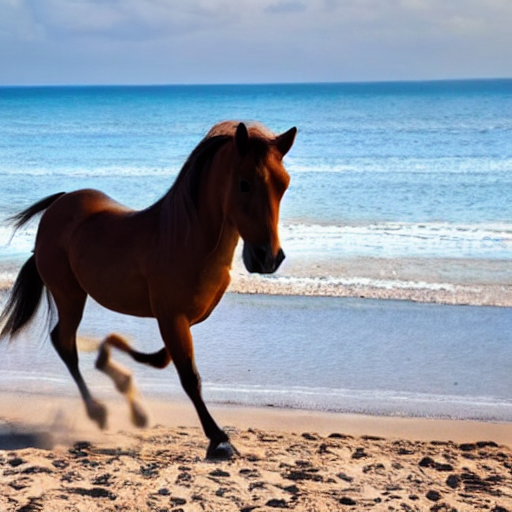
\includegraphics[width=0.13\linewidth]{img/esd_orig_horse.png} &
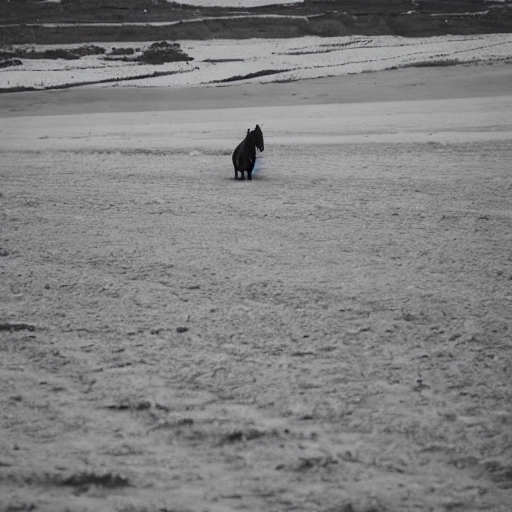
\includegraphics[width=0.13\linewidth]{img/esd_unlearn_horse.png} &
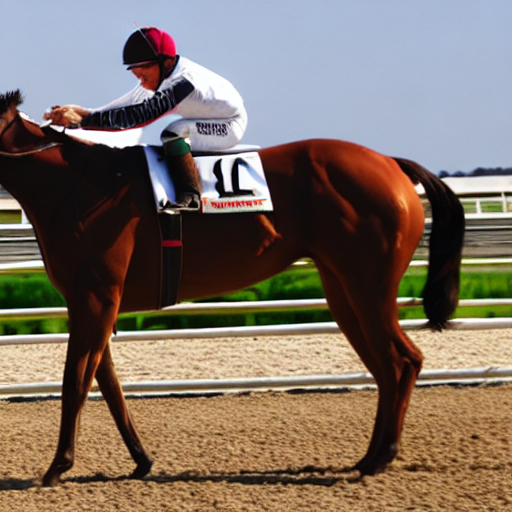
\includegraphics[width=0.13\linewidth]{img/esd_orig_nohorse.png} &
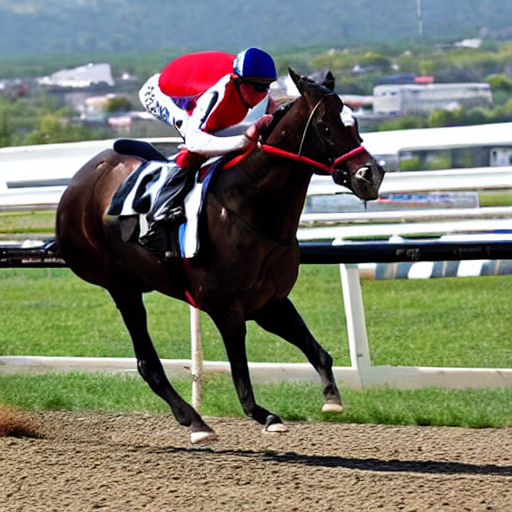
\includegraphics[width=0.13\linewidth]{img/esd_unlearn_nohorse.png} \\

\textbf{AdvUnlearn} &
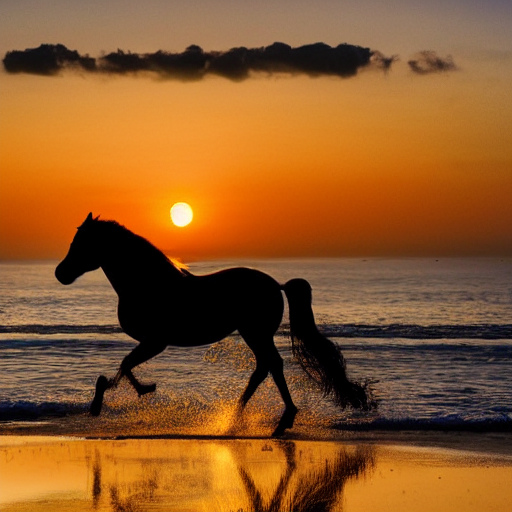
\includegraphics[width=0.13\linewidth]{img/adv_orig_horse.png} &
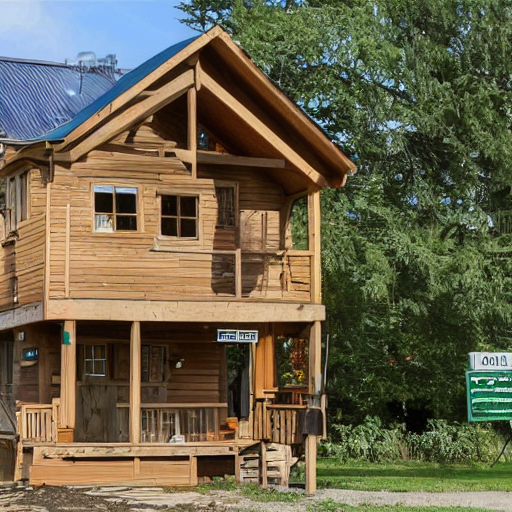
\includegraphics[width=0.13\linewidth]{img/adv_unlearn_horse.png} &
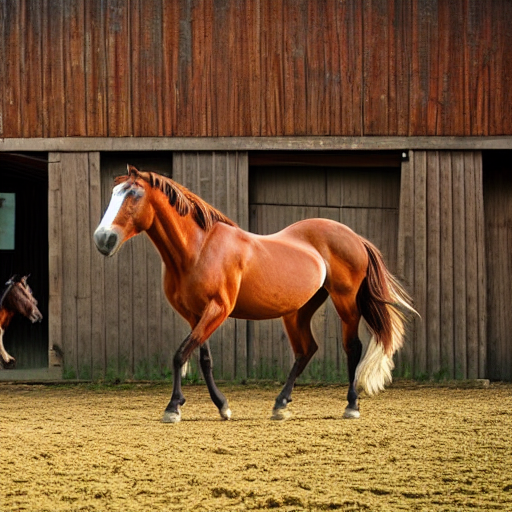
\includegraphics[width=0.13\linewidth]{img/adv_orig_nohorse.png} &
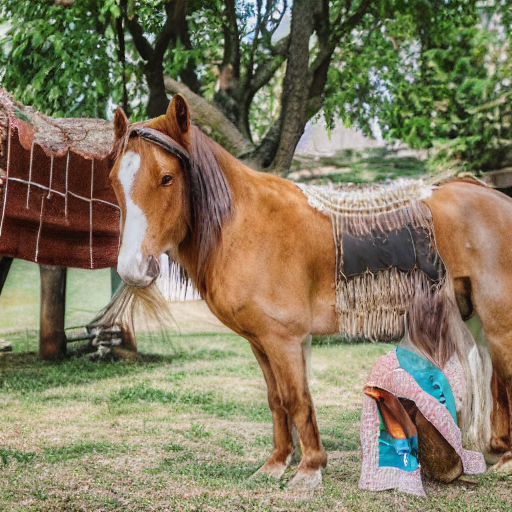
\includegraphics[width=0.13\linewidth]{img/adv_unlearn_nohorse.png} \\

\textbf{STEREO} &
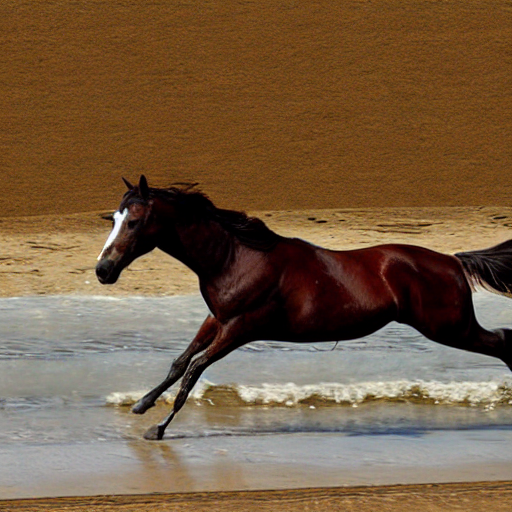
\includegraphics[width=0.13\linewidth]{img/stereo_orig_horse.png} &
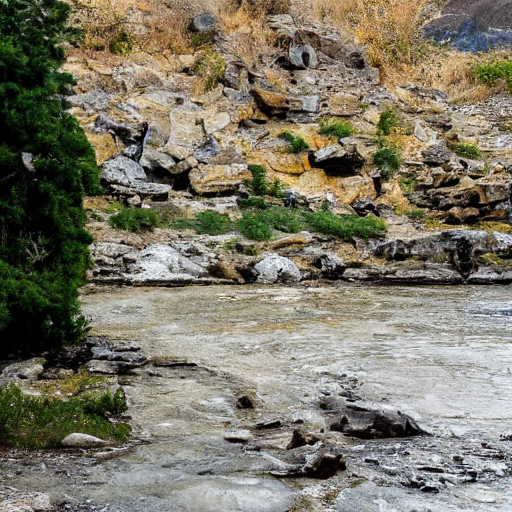
\includegraphics[width=0.13\linewidth]{img/stereo_unlearn_horse.png} &
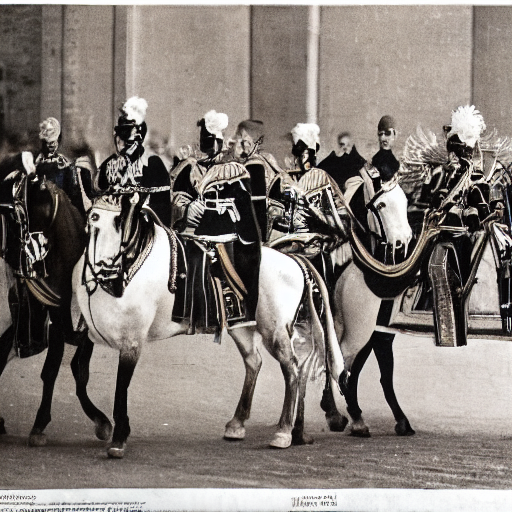
\includegraphics[width=0.13\linewidth]{img/stereo_orig_nohorse.png} &
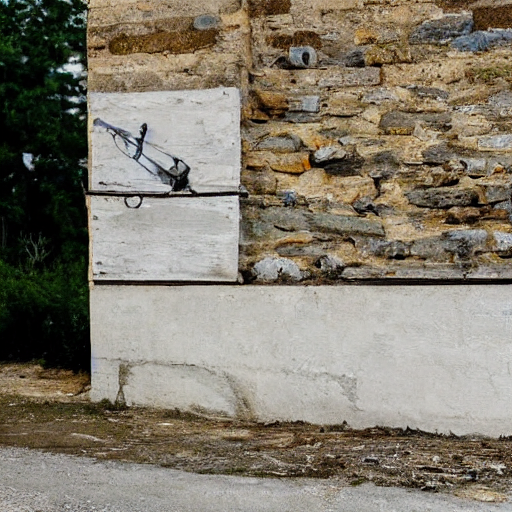
\includegraphics[width=0.13\linewidth]{img/stereo_unlearnnohorse.png} \\

\textbf{SAeUron} &
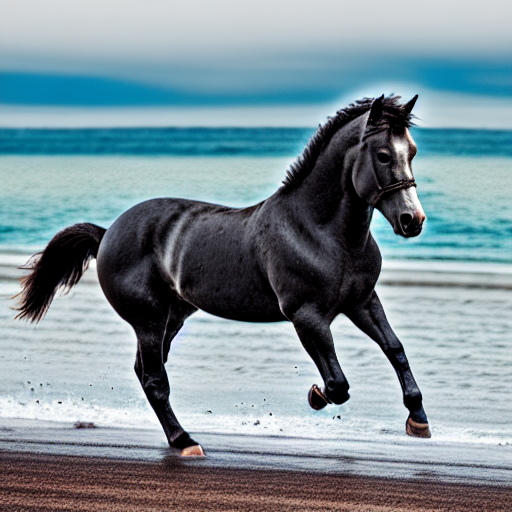
\includegraphics[width=0.13\linewidth]{img/saeuron_orig_horse.png} &
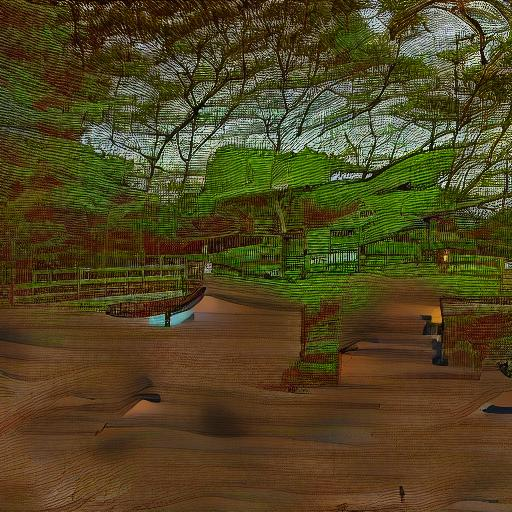
\includegraphics[width=0.13\linewidth]{img/saeuron_unlearn_horse.jpg} &
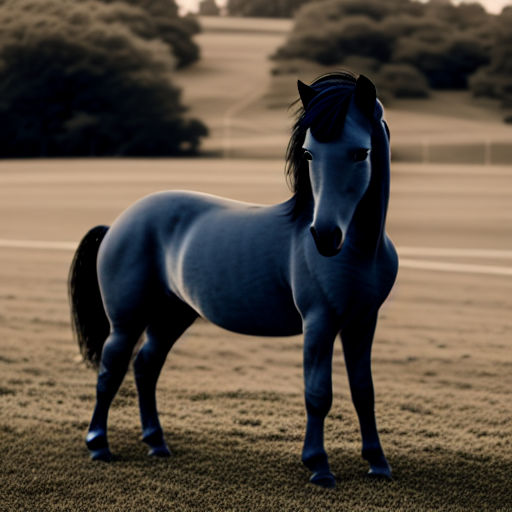
\includegraphics[width=0.13\linewidth]{img/saeuron_orig_nohorse.png} &
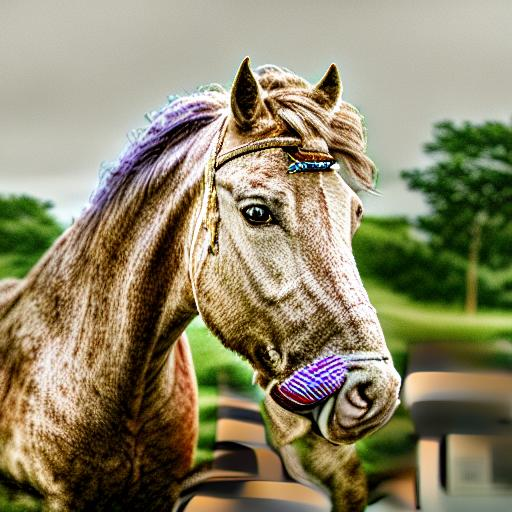
\includegraphics[width=0.13\linewidth]{img/saeuron_unlearn_nohorse.jpg} \\

\end{tabular}
\caption{
\textbf{Concept entanglement manifests as two coupled effects.}
Each row shows a different unlearning method applied to erase \texttt{horse}.
\emph{Left pair} (prompt with ``horse''): all methods successfully suppress the target concept.
\emph{Right pair} (prompt without ``horse'' but with correlated context): methods with localized erasure (ESD, SAeUron) regenerate horses through contextual leakage, while robust methods (STEREO) suppress leakage but degrades semantically neighboring concepts such as \texttt{donkey} and \texttt{zebra}. These two effects are dual consequences of representational overlap between the target concept and its semantic neighbors. %\varun{make figure much much smaller?}
}
\label{fig:concept_leakage}
\end{figure*}
\end{comment}
\section{The Robustness--Retention Trade-off: A Formal Impossibility Result}
\label{sec:tradeoff}

We now formalize the coupling observed in~\cref{sec:motivation} as a provable lower bound on the trade-off between erasure robustness and concept preservation. The governing quantity is the \emph{concept overlap coefficient} $\kappa$, which measures the fraction of the target concept's activation region shared with the remaining concepts.

\subsection{Setup and Definitions}
\label{subsec:definitions}

Let $\mathcal{D}_\theta$ be a pretrained text-to-image diffusion model with U{-}Net noise predictor $\boldsymbol{\epsilon}_\theta$ and text encoder $f_\psi : \mathcal{P} \to \mathbb{R}^d$, where $\mathcal{P}$ is the space of text prompts. 
For a prompt $p \in \mathcal{P}$, we denote its embedding by $\mathbf{e}_p = f_\psi(p) \in \mathbb{R}^d$, and write $p_\theta(\mathbf{x} \mid p)$ for the conditional distribution over images induced by $\mathcal{D}_\theta$.
Let $\mathcal{D}_{\hat\theta}$ denote a concept-erased model (CEM) obtained by applying an unlearning procedure. 
We correspondingly write $\boldsymbol{\epsilon}_{\hat\theta}$ for the edited U-Net and $p_{\hat\theta}(\mathbf{x} \mid p)$ for the induced conditional distribution. 

\noindent{\bf Concept activation regions.}
%For a fixed probe layer $\ell^*$ and denoising timestep $t^*$, let $\boldsymbol{\Phi}_\theta(p)$ denote the mean-pooled cross-attention activation produced by prompt $p \in \mathcal{P}$, where $\mathcal{H} := \mathbb{R}^{d_{\ell^*}}$ is the activation space at layer $\ell^*$ and $d_{\ell^*}$ is the per-token channel dimension at that layer. Each concept $c \in \mathcal{C}$ is associated with its \emph{activation region} $\mathcal{R}_c \subseteq \mathcal{H}$ produced by prompts whose generated images contain $c$. The formal construction is given in~\cref{app:concept_regions}.
For a fixed probe layer $\ell^*$ and denoising timestep $t^*$, let $\boldsymbol{\Phi}^{\ell^*}_\theta(p)$ denote the mean-pooled cross-attention activation produced by prompt $p \in \mathcal{P}$. 
For a concept $c \in \mathcal{C}$, we define its \emph{activation region} at layer $\ell^*$ as
\begin{equation}
    \mathcal{R}_c (\ell^*)
    \;=\;
    \Bigl\{
        \boldsymbol{\Phi}^{\ell^*}_\theta(p)
        \;\Big|\;
        p \in \mathcal{P},\;
        \mathbb{O}_{\mathcal{X}}\!\left(\mathbf{x}_{\theta}(p),\, c\right) = 1
    \Bigr\}
    \;\subseteq\; \mathbb{R}^{d_{\ell^*}},
\end{equation}
% \ali{this also depends on $\ell^*,t^*$} 
% \varun{bold-facing issues here too}
where (i) $\mathbb{O}_{\mathcal{X}} : \mathcal{X} \times \mathcal{C} \to \{0,1\}$ is an oracle indicating whether concept $c$ is present in image $x$, (ii) $\mathbf{x}_{\theta}(p) \sim p_{\theta}(\cdot \mid p)$ denotes an image sampled from $\mathcal{D}_\theta$ conditioned on prompt $p$, and (iii) $d_{\ell^*}$ is the per-token channel dimension at layer at layer $\ell^*$.
We also define the closed $\rho$-neighborhood of $\mathcal{R}_c$ as:
\begin{equation}
    \mathcal{R}_c^{(\rho)} (\ell^*)
    \;=\;
    \bigl\{\mathbf{h} \in \mathbb{R}^{d_{\ell^*}} \;\big|\;
    \inf_{\mathbf{r}  \in \mathcal{R}_c}\|\mathbf{h} - \mathbf{r}\|_2 \leq \rho\bigr\}
\end{equation}

When clear from context, we drop $\ell^*$ and simply write $\boldsymbol{\Phi}_\theta(p)$ and $\mathcal{R}_c^{(\rho)}$ for brevity.
The key quantity governing the trade-off is the degree of representational overlap between the target concept and other concepts, defined as follows. 


\begin{definition}
\label{def:overlap}
The \emph{entanglement coefficient} of target concept $c_u$ with fattening radius $\rho > 0$ is
\[
    \kappa(c_u,\,\rho)
    \;=\;
    \frac{
        \mathrm{vol}\!\left(
            \mathcal{R}_{c_u}^{(\rho)}
            \cap
            \bigcup_{c' \in \mathcal{C} \setminus \{c_u\}} \mathcal{R}_{c'}^{(\rho)}
        \right)
    }{
        \mathrm{vol}\!\left(\mathcal{R}_{c_u}^{(\rho)}\right)
    },
\]
where $\mathrm{vol}(\cdot)$ denotes the $n$-dimensional volume of subsets of $\mathbb{R}^n$.
\end{definition}

\noindent Intuitively, $\kappa \in [0,1]$ measures what fraction of the target concept's representational footprint overlaps with that of other concepts in the model. When $\kappa = 0$, the concept is fully disentangled and can in principle be erased without collateral damage. When $\kappa > 0$, any edit that displaces activations in $\mathcal{R}_{c_u}$ will inevitably disturb overlapping portions of other concepts' activation regions.
This formulation aggregates overlap across all concepts. In practice, however, the contribution to $\kappa$ is dominated by concepts that occupy nearby regions of the activation space and distant concepts contribute negligibly to the intersection. 

\noindent{\bf Quantifying entanglement.}
\Cref{tab:kappa} reports $\hat\kappa$, an empirical lower-bound estimator of the entanglement coefficient $\kappa$ defined above, for five target concepts.
% \Cref{tab:kappa} reports the estimated lower-bound for entanglement coefficient $\hat\kappa$ for five target concepts. \varun{what is $\hat\kappa$? not defined}
Each $\hat\kappa(c_u)$ is computed as the fraction of activation samples from $c_u$ that lie within a fattening radius $\rho_{c_u}$ of any activation from a discovered neighbor concept; the full estimation procedure, choice of $\rho_{c_u}$, and per-target results are detailed in~\cref{app:kappa_per_target}.
The four animal subtypes (\texttt{dog}, \texttt{bear}, \texttt{horse}, \texttt{cat}) exhibit substantial overlap with fine-grained variants (e.g., \texttt{donkey}, \texttt{mare} for \texttt{horse}), while \texttt{castle} exhibits significantly lower overlap. % despite having semantically related concepts. 
This heterogeneity in $\hat\kappa$ defines the regime in which~\Cref{thm:tradeoff} predicts collateral damage should scale: erasing a high-$\hat\kappa$ concept incurs substantially larger preservation error than erasing a low-$\hat\kappa$ one. We validate this hypothesis in~\cref{subsec:kappa_scaling}. 
%Estimation details and sensitivity analyses are in~\cref{app:kappa_estimation}.

We now define the two desiderata that any unlearning method must satisfy:

\begin{definition}[$\varepsilon$-robust unlearning]
\label{def:robust}
The CEM $\mathcal{D}_{\hat\theta}$ achieves \emph{$\varepsilon$-robust unlearning} of concept $c_u$ if, for all prompts $p \in \mathcal{P}$,% (including indirect prompts that do not explicitly mention $c_u$),
\begin{equation}
    \Pr_{\mathbf{x} \sim p_{\hat\theta}(\cdot \mid p)}
\!\left[
\mathbb{O}_{\mathcal{X}}(\mathbf{x} ,\, c_u) = 1
\right]
\;\leq\; \varepsilon.
\end{equation}
% where $\mathbb{O}_{\mathcal{X}} : \mathcal{X} \times \mathcal{C} \to \{0,1\}$ is the oracle concept detector \varun{already defined above; so maybe remove here?}. 
% The worst-case quantifier reflects an adversarial threat model (see~\cref{subsec:setup}) \ali{again the section reference is too general. use the specific subsections when possible}.  % we additionally report the corresponding average-case quantity UA.
\end{definition}
\noindent{\bf Intuition.} Definition~\ref{def:robust} considers an unlearned model $\varepsilon$-robust if no prompt generates the erased concept with probability greater than $\varepsilon$. See~\cref{app:concept_regions} for more details on the oracle.

\begin{definition}[$\gamma$-concept preservation]
\label{def:neighbor}
Let $\mathcal{P}_{c'} \subseteq \mathcal{P}$ denote the set of prompts associated with concept $c'$, and let $\mathcal{P}_{-u}$ denote the \emph{non-target prompt distribution}, defined as the uniform mixture
$\mathcal{P}_{-u} \;=\; \tfrac{1}{|\mathcal{C}\setminus\{c_u\}|}\sum_{c' \in \mathcal{C}\setminus\{c_u\}} \mathcal{P}_{c'}$.
The CEM $\mathcal{D}_{\hat\theta}$ achieves \emph{$\gamma$-concept preservation} with respect to layer ${\ell^*}$ if
\begin{equation}
    \mathbb{E}_{p \sim \mathcal{P}_{-u}}\!\left[\bigl\|\boldsymbol{\Phi}^{\ell^*}_{\hat\theta}(p) - \boldsymbol{\Phi}^{\ell^*}_\theta(p)\bigr\|_2\right]
    \;<\; \gamma.
\end{equation}
% Let $\mathcal{P}_{c'} \subseteq \mathcal{P}$ denote the set of prompts associated with concept $c'$. 
% The CEM $\mathcal{D}_{\hat\theta}$ achieves \emph{$\gamma$-concept preservation} with respect to layer ${\ell^*}$ if, for all $c' \in \mathcal{C} \setminus \{c_u\}$,
% \begin{equation}
%     \mathbb{E}_{p \sim \mathcal{P}_{c'}}\!\left[\bigl\|\boldsymbol{\Phi}^{\ell^*}_{\hat\theta}(p) - \boldsymbol{\Phi}^{\ell^*}_\theta(p)\bigr\|_2\right]
%     \;<\; \gamma.
% \end{equation}
\end{definition}

\noindent{\bf Intuition.} An unlearned model has $\gamma$-concept preservation at a specific layer if, on average over prompts from all non-target concepts, the displacement of their representations at that layer remains smaller than $\gamma$.



\subsection{Main Result: The Trade-off Lower Bound}
\label{subsec:main_result}

In this section, we show that $\varepsilon$-robust unlearning and $\gamma$-concept preservation are fundamentally in tension.
We begin by stating two mild regularity assumptions that formalize how perturbations in activation space affect generation.

\begin{assumption}[Lipschitz continuity of generation]
\label{asm:lip}
Let $\mathcal{H} = \mathbb{R}^{d_{\ell^*}}$ denote the cross-attention activation space at layer $\ell^*$.
For each concept $c \in \mathcal{C}$, the generation probability is Lipschitz continuous with respect to activations:
\begin{equation}
    \left|
    \Pr[\mathbb{O}_{\mathcal{X}}(\mathbf{x}_{\mathbf{h}},c)=1]
    -
    \Pr[\mathbb{O}_{\mathcal{X}}(\mathbf{x}_{\mathbf{h}'},c)=1]
    \right|
    \leq
    L\|\mathbf{h}-\mathbf{h}'\|_2,
    \quad \forall \mathbf{h}, \mathbf{h}' \in \mathcal{H}.
\end{equation}

where $\mathbf{x}_{\mathbf{h}} \sim p_\theta(\cdot \mid \boldsymbol{\Phi}_\theta^{-1}(\mathbf{h}))$
denotes an image generated from an activation vector $\mathbf{h}$.

\end{assumption}

\begin{assumption}[Minimum displacement for erasure]
\label{asm:edit}
Any unlearning edit $\theta \mapsto \hat{\theta}$ that achieves $\varepsilon$-robust unlearning of $c_u$ must displace activations within $\mathcal{R}_{c_u}$ by at least $\Delta>0$:
\begin{equation}
\label{eq:delta_lower}
    \forall p \in \mathcal{P}
    \text{ such that }
    \boldsymbol{\Phi}_{\theta}(p)\in \mathcal{R}_{c_u}:
    \quad
    \|\boldsymbol{\Phi}_{\hat{\theta}}(p)-\boldsymbol{\Phi}_{\theta}(p)\|_2
    \geq
    \Delta .
\end{equation}
\end{assumption}
We empirically verify assumption~\ref{asm:lip} across natural prompt variations and assumption~\ref{asm:edit} across five unlearning methods erasing \texttt{horse}; all measured pairs satisfy Lipschitz with a small empirical constant, 
% and displacement propagates to semantic neighbors more than to controls. 
and displacement propagates to other concepts through shared activation structure.
Full details are in~\cref{app:lipschitz,app:displacement}.


\begin{theorem}[Robustness--Retention trade-off]
\label{thm:tradeoff}
Let Assumptions~\ref{asm:lip} and~\ref{asm:edit} hold with constants $L$ and $\Delta$.
Let $\rho > 0$ be the fattening radius from Definition~\ref{def:overlap}.
Suppose $\mathcal{D}_{\hat\theta}$ achieves $\varepsilon$-robust unlearning of $c_u$
(Definition~\ref{def:robust}).
%Then for any concept $c' \in \mathcal{C}$ with $c' \neq c_u$, the expected activation displacement satisfies
Then the aggregate collateral displacement over non-target concepts satisfies
\begin{equation}
    \mathbb{E}_{p\sim \mathcal{P}_{-u}}
    \left[
\|\boldsymbol{\Phi}_{\hat{\theta}}(p)-\boldsymbol{\Phi}_{\theta}(p)\|_2
    \right]
    \geq
    \kappa(c_u,\rho)\cdot \Delta .
\end{equation}
% where $\kappa(c_u,\rho)$ is the entanglement coefficient from Definition~\ref{def:overlap}.
Consequently, achieving $\gamma$-concept preservation(Definition~\ref{def:neighbor}) requires
% where $\mathcal{P}_{-u}$ denote the distribution over non-target prompts. Consequently, achieving $\gamma$-concept preservation (Definition~\ref{def:neighbor}) requires
\begin{equation}
\label{eq:tradeoff}
    \boxed{
    \gamma \;\geq\; \kappa(c_u,\rho)\cdot\frac{1-\varepsilon}{L}.
    }
\end{equation}
Equivalently, when $\kappa(c_u,\rho) > 0$, achieving both $\varepsilon$-robustness and $\gamma$-concept preservation simultaneously requires
\begin{equation}
\label{eq:tradeoff_eps}
    \varepsilon \;\geq\; 1 - \frac{L\gamma}{\kappa(c_u,\rho)}.
\end{equation}
\end{theorem}

\begin{proof}[Proof sketch]
Assumptions~\ref{asm:lip} and~\ref{asm:edit} together force every activation in $\mathcal{R}_{c_u}$ to be displaced by at least $\Delta \geq (1-\varepsilon)/L$ under any $\varepsilon$-robust edit. By Definition~\ref{def:overlap}, a $\kappa(c_u,\rho)$-fraction of $\mathcal{R}_{c_u}^{(\rho)}$ lies in the support of $\mathcal{P}_{-u}$, so this displacement propagates to at least a $\kappa(c_u,\rho)$-fraction of $\mathcal{P}_{-u}$'s mass, yielding $\mathbb{E}_{p\sim\mathcal{P}_{-u}}[\|\Phi_{\hat\theta}(p)-\Phi_\theta(p)\|_2] \geq \kappa(c_u,\rho)(1-\varepsilon)/L$. Definition~\ref{def:neighbor} then gives the bound on $\gamma$. The full proof including the regularity assumption is in Appendix~\ref{app:proof}.
\end{proof}
% \begin{proof}[Proof sketch]
% By assumption~\ref{asm:lip}, %$\varepsilon$-robust unlearning requires displacing all activations in $\mathcal{R}_{c_u}$ by at least $\Delta = (1-\varepsilon)/L$. This displacement propagates to the fraction $\kappa(c_u,\delta)$ of $\mathcal{R}_{c'}$ that overlaps with $\mathcal{R}_{c_u}^{(\rho)}$, minus at most $\delta$ due to inter-concept distance. 
% $\varepsilon$-robust unlearning requires displacing all activations in $\mathcal{R}_{c_u}$ by at least $\Delta = (1-\varepsilon)/L$. By Definition~\ref{def:overlap}, a fraction $\kappa(c_u,\rho)$ of the fattened region $\mathcal{R}_{c_u}^{(\rho)}$ overlaps with non-target concept regions. This displacement therefore affects at least a $\kappa(c_u,\rho)$ fraction of the shared activation mass, yielding an aggregate collateral displacement of at least $\kappa(c_u,\rho)\cdot \Delta$.
% % For any neighbor $c'$ whose fattened activation region overlaps with $\mathcal{R}_{c_u}^{(\rho)}$, the displacement in the overlap region propagates to $\mathcal{R}_{c'}$, yielding a lower bound proportional to the overlap fraction $\kappa(c_u,\delta)$ minus the inter-concept distance $\delta$. Then substituting $\Delta = (1-\varepsilon)/L$ yields the stated bound on $\gamma$. 
% Full proof is given in Appendix~\ref{app:proof}.
% \end{proof}

\subsection{Consequences and Interpretation}
\label{subsec:consequences}

% \noindent{\bf Impossibility of perfect unlearning with perfect retention.}
\noindent{\bf Limitations of simultaneous robust erasure and utility preservation.}
Based on~\Cref{thm:tradeoff}, simultaneous perfect erasure and perfect retention is infeasible whenever concepts are entangled:
\begin{corollary}[Impossibility result]
\label{cor:impossibility}
%If $\kappa(c_u, \delta) > 0$ and $\delta < \kappa(c_u,\delta)/L$, 
If $\kappa(c_u,\rho) > 0$,
then no unlearning method can simultaneously achieve $\varepsilon = 0$ (perfect erasure) and $\gamma = 0$ (perfect neighbor preservation).
\end{corollary}

\begin{proof}
Setting $\varepsilon = 0$ in Eq.~\eqref{eq:tradeoff} gives 
% $\gamma \geq \kappa(c_u,\delta)/L - \delta > 0$ 
$\gamma \geq \kappa(c_u,\rho)/L > 0$
under the stated conditions.
\end{proof}

\noindent{\bf The Pareto frontier.}
Eq.~\eqref{eq:tradeoff_eps} defines a \emph{feasibility boundary} in the $(\varepsilon, \gamma)$ plane: no method can simultaneously achieve an erasure robustness below $\varepsilon$ and a neighbor preservation error below $\gamma$ unless the pair $(\varepsilon, \gamma)$ lies above the curve
$\gamma = \kappa \cdot \frac{1-\varepsilon}{L}.$
Different unlearning methods correspond to different operating points on or above this curve: aggressive methods achieve small $\varepsilon$ at the cost of large $\gamma$, occupying the upper-left of the frontier; conservative methods accept large $\varepsilon$ to maintain small $\gamma$, occupying the lower-right.
In Section~\ref{sec:experiment}, we verify that the empirically observed operating points across seven methods are consistent with this predicted boundary.


% \noindent{\bf Empirical validation.}
% To verify that concept activation regions are well-defined empirical objects, we extract cross-attention activations from Stable Diffusion v1.4 at the mid-block layer (\texttt{mid\_block.attentions.0}) at step $t^*{=}25$ of 50 DDIM steps for 10 concepts, each prompted with 50 shared templates differing only in the concept word.
% Figure~\ref{fig:umap} shows that concepts with nearby activation centroids in the extracted cross-attention space from neighboring clusters. For example,: \texttt{horse}, \texttt{pony}, and \texttt{donkey} form a dense equine cluster, while \texttt{castle} is well-separated from all animal concepts. This provides empirical support that concept activation regions are coherent geometric objects in $\mathcal{H}$.


% Empirical evidence that these activation regions correspond to coherent geometric structure is shown in~\cref{fig:umap}; full construction details and discussion are deferred to Appendix~\ref{app:activation_regions}.

% \varun{this is EXCELLENT!!! i would move this figure to the intro; move the discussion of the figure (this empirical validation paragraph) to the appendix, but refer to the figure in a single line in this part of the paper to show that "empirical validation shows that these definitions are real"}


% We formalize the notion that concepts occupy regions in the model's internal activation space, and that these regions can overlap for semantically related concepts.

% \varun{what does this activation region capture? similarly what does the activation function capture?}
% \begin{definition}[Concept activation region]
% \label{def:activation}
% Fix a UNet layer $\ell^*$ and denoising timestep $t^* \in \{1,\ldots,T\}$. The \emph{concept activation function} is
% \[
%     \boldsymbol{\Phi}_\theta : \mathcal{T} \longrightarrow \mathcal{Z}, \qquad
%     \boldsymbol{\Phi}_\theta(p) \;=\; \mathrm{A}_\theta(p,\, \ell^*,\, t^*),
% \]
% where $\mathrm{A}_\theta(p,\ell,t)$ denotes the cross-attention output at layer $\ell$ and timestep $t$ \varun{what is $p$?}. The \emph{activation region} of concept $c$ is
% \[
%     \mathcal{R}_c \;=\; \bigl\{\, \boldsymbol{\Phi}_{\theta^*}(p) \;\big|\;
%     p \in \mathcal{T},\; \mathbb{O}_\mathcal{X}(f_\boldsymbol{\Phi}(p), c) = 1
%     \,\bigr\} \;\subseteq\; \mathcal{Z},
% \]
% where $\mathbb{O}_\mathcal{X} : \mathcal{X} \times \mathcal{C} \to \{0,1\}$ is the ground-truth oracle indicating whether concept $c$ is present in image $x$.
% \end{definition}

% \begin{definition}[Semantic neighborhood]
% \label{def:neighborhood}
% The \emph{semantic neighborhood} of concept $c$ at radius $\delta > 0$ is
% \[
%     \mathcal{N}_\delta(c) \;=\; \bigl\{\, c' \in \mathcal{C}
%     \;\big|\; c' \neq c, \;
%     d_\mathcal{Z}\!\left(\mathcal{R}_c,\, \mathcal{R}_{c'}\right)
%     < \delta \,\bigr\},
% \]
% where $d_\mathcal{Z}(A,B) = \inf_{a \in A, b \in B}\|a - b\|_2$ is the set distance in $\mathcal{Z}$. \varun{$\mathcal{R}_{c'}$ is not defined?}
% \end{definition}
% \begin{definition}[Semantic neighborhood]
% \label{def:neighborhood}
% For a concept $c \in \mathcal{C}$ and radius $\delta > 0$, its \emph{semantic neighborhood}
% is
% \begin{equation}
%     \mathcal{N}_{\delta}(c)
% \;=\;
% \left\{
% c' \in \mathcal{C}
% \;\middle|\;
% c' \neq c,\;
% d_{\mathcal{H}}(\mathcal{R}_c,\,\mathcal{R}_{c'}) < \delta
% \right\},
% \end{equation}
% where $\mathcal{R}_{c'}$ is the activation region of concept $c'$ as in
% Definition~\ref{def:activation}, and
% \begin{equation}
%     d_{\mathcal{H}}(A,B) \;=\; \inf_{a \in A,\; b \in B}\|a - b\|_2
% \end{equation}

% \ali{since we use infimum in the definition, Figure 1 might be misleading.}
% is the point set distance in $\mathcal{H}$.
% \end{definition}

% Figure~\ref{fig:distance_matrix} reports the pairwise centroid cosine distance between 10 example concept activation regions, ordered by hierarchical clustering to reveal block structure.
% Two patterns emerge that directly bear on the trade-off.
% First, concepts within the same semantic category have small centroid distances: \texttt{horse}$\leftrightarrow$\texttt{pony} ($0.158$), \texttt{horse}$\leftrightarrow$\texttt{donkey} ($0.329$), \texttt{dog}$\leftrightarrow$\texttt{cat} ($0.282$), \texttt{car}$\leftrightarrow$\texttt{truck} ($0.400$). These small distances suggest substantial representational overlap, predicting that erasing any concept in these clusters will displace activations into neighboring concepts' regions. Second, semantically isolated concepts such as \texttt{castle} have centroid distances exceeding $0.65$ to all animal concepts, implying $\kappa \approx 0$ and predicting minimal collateral damage under erasure. We verify these predictions empirically in~\cref{sec:experiment}.
% \ali{this seems like a good empirical evidence to me, but a reviewer might raise the concern than your definitions are based on infimum while the empricial distance is based on average values.}
% The four animal concepts cluster at high entanglement ($\hat\kappa \in [0.77, 0.89]$): their activation regions overlap substantially with fine-grained subtypes and near-synonyms in the same taxonomic category, such as \texttt{puppy} and \texttt{labrador} for \texttt{dog}, or \texttt{donkey}, \texttt{foal}, and \texttt{mare} for \texttt{horse}. \texttt{castle}, by contrast, exhibits substantially lower entanglement ($\hat\kappa = 0.27$) despite having a similar number of discovered architectural neighbors (\texttt{fortress}, \texttt{palace}, \texttt{citadel}, \texttt{keep}, \texttt{manor}): these concepts are semantically related but occupy more distinct regions of activation space. 
% \varun{next sentence comes out of the blue; perhaps do not need it here?}
% \Cref{thm:tradeoff} predicts that collateral damage from erasing a high-$\hat\kappa$ concept will be substantially greater than from erasing a low-$\hat\kappa$ one; we verify this in~\cref{sec:experiment}. Full estimation details are in~\cref{app:kappa_estimation}.
% \begin{table}[t]
% \centering
% \small
% \begin{tabular}{lccc}
% \toprule
% Concept & $\hat\kappa$ & Silhouette & Neighbors \\
% \midrule
% % pony    & 0.46 & 0.47 & horse, donkey \\
% dog     & 0.89 & 0.54 & puppy, labrador \\
% % donkey  & 0.04 & 0.66 & horse, pony, deer \\
% % car     & 0.02 & 0.59 & dog, cat, truck, tower \\
% % deer    & 0.02 & 0.71 & donkey \\
% bear    & 0.82 & 0.70 & black bear, brown bear, grizzly\\
% horse   & 0.81 & 0.43 & donkey,foal,mare \\
% cat     & 0.77 & 0.53 & kitten, panther \\
% % truck   & 0.00 & 0.76 & car, tower \\
% castle  & 0.27 & 0.89 & citadel, fortress, keep, manor, palace \\
% \bottomrule
% \end{tabular}
% \caption{Estimated entanglement coefficient $\hat\kappa$ and  silhouette score \varun{what is this?} for each concept, computed on mean-pooled 
% cross-attention activations with cosine distance. Higher $\hat\kappa$ indicates greater representational overlap with semantic neighbors; higher silhouette 
% indicates a more isolated activation region. See~\cref{app:kappa_estimation} for estimation details.}
% \label{tab:kappa}
% \end{table}


\section{Experiments}
\label{sec:experiment}
We design our experiments to answer three questions, each tied to a component of our contribution:

% \ali{for each following question, we should specify the sections that address them.}  \varun{+1}
%\varun{if we have a squishsquishenumerate instead of squishenumerate, use that?}

\begin{squishenumerate}
    \item[\textbf{Q1.}] Does the robustness--retention trade-off predicted by~\cref{thm:tradeoff} manifest empirically across a broad set of unlearning methods? (\cref{subsec:tradeoff_real})
    \item[\textbf{Q2.}] Does the severity of the trade-off vary with the estimated entanglement coefficient $\hat\kappa$, as predicted by the theorem's dependence on $\kappa$? (\cref{subsec:kappa_scaling})
    % \ali{i think another important question that we investigate is whether the assumptions that we make for our theoretical results hold.}
    \item[\textbf{Q3.}] Do the Lipschitz continuity (\cref{asm:lip}) and minimum displacement (\cref{asm:edit}) assumptions underlying~\cref{thm:tradeoff} hold empirically? (\cref{app:lipschitz,app:displacement})
\end{squishenumerate}
\noindent \textbf{Summary of findings.} Across seven unlearning methods and target concepts spanning $\hat\kappa \in [0.27, 0.89]$, no method simultaneously achieves strong erasure (UA $> 90\%$) and strong neighbor preservation (NP $> 80\%$); methods instead occupy distinct regions of a Pareto frontier consistent with~\Cref{thm:tradeoff} (Q1). Trade-off severity scales monotonically with $\hat\kappa$ for methods that operate near the theoretical bound (Spearman $\rho = -1.0$ for robust fine-tuning), while methods with smaller effective displacement $\Delta$ show weaker $\hat\kappa$-dependence (Q2). The Lipschitz and minimum-displacement assumptions hold empirically on the prompt distributions and methods we evaluate (Q3).


\subsection{Experimental Setup}
\label{subsec:setup}

\noindent{\bf Base model and target concepts.}
We use CompVis Stable Diffusion v1.4~\citep{rombach2022high} as the base model $\mathcal{D}_\theta$. Following~\citep{gandikota2023erasing}, all generation uses 50 DDIM steps with guidance scale 7.5; 
% \ali{if these are commong settings for prior work it is good to add references to support these choices.} 
full details in~\cref{app:implementation}.
We select five target concepts spanning the range $\hat\kappa \in [0.27, 0.89]$ identified in~\cref{tab:kappa}: 
four high-$\hat\kappa$ animal-subtype concepts (\texttt{horse}, \texttt{dog}, \texttt{cat}, \texttt{bear}, $\hat\kappa \in [0.77, 0.89]$) and one low-$\hat\kappa$ architectural concept (\texttt{castle}, $\hat\kappa = 0.27$). Each target is evaluated against its discovered concept neighborhood and a 10-concept control set (\cref{tab:kappa_per_target}); per-target prompt sets are detailed in~\cref{app:eval_pipeline}. 

% \varun{assume that the reviewers will ask for more concepts, covering more regions of the $\kappa$ spectrum, so please run these evaluations ahead of time!}
% \begin{squishenumerate}
%     \item \emph{High-$\hat\kappa$ animal-subtype concepts}: \texttt{horse}, \texttt{dog}, \texttt{cat}, and \texttt{bear}. Each lies in a semantically dense neighborhood of fine-grained subtypes and near-synonyms (e.g., \texttt{donkey}, and \texttt{mare} for \texttt{horse}).
%     \item \emph{Low-$\hat\kappa$ architectural concept}: 
%     \texttt{castle}, whose architectural neighbors (\texttt{fortress}, \texttt{palace}, \texttt{citadel}) 
%     occupy related but more distinct activation regions.
% \end{squishenumerate}
% For each target, evaluation is performed against the 10-concept neighborhood and 3-concept control set defined in~\cref{tab:kappa}; per-target prompt sets are detailed in~\cref{app:eval_pipeline}.

\noindent{\bf Unlearning methods.}
We benchmark seven methods spanning two mechanism families: fine-tuning methods (ESD~\citep{gandikota2023erasing}, 
SalUn~\citep{fan2023salun}, 
EDiff~\citep{wu2024erasediff}, 
AdvUnlearn~\citep{zhang2024defensive}, 
STEREO~\citep{srivatsan2025stereo}) 
and inference-time methods 
(SEOT~\citep{li2024get}, SAeUron~\citep{cywinski2025saeuron}). 
AdvUnlearn and STEREO incorporate adversarial training to target the aggressive-erasure end of the trade-off. Training protocols and hyperparameters follow the original publications; see~\cref{app:implementation}.
% We benchmark seven methods spanning two mechanism families. 
% \emph{Fine-tuning methods} modify model weights through gradient updates: 
% ESD~\citep{gandikota2023erasing}, %FMN~\citep{zhang2024forget}, 
% % CA~\citep{vinker2023concept}, 
% % UCE~\citep{gandikota2024unified}, 
% % SA~\citep{heng2023selective}, 
% SalUn~\citep{fan2023salun},
% EDiff~\citep{wu2024erasediff}.
% and the adversarially-robust variants AdvUnlearn~\citep{zhang2024defensive} and 
% STEREO~\citep{srivatsan2025stereo}. 
% %and SHS~\citep{wu2024scissorhands}. 
% % \emph{Inference-time methods} intervene during generation without modifying weights: SPM~\citep{lyu2024one}, 
% \emph{Inference-time methods} intervene during generation without full-model fine-tuning: 
% SEOT~\citep{li2024get}, and SAeUron~\citep{cywinski2025saeuron},  which uses sparse autoencoder feature ablation applied at inference. 
% AdvUnlearn and STEREO specifically target the aggressive-erasure end of the trade-off by incorporating adversarial training, allowing us to probe whether robustness gains come at measurable cost to neighbor preservation.

\noindent{\bf Evaluation.}
We measure seven metrics spanning the two axes of~\cref{thm:tradeoff} and these metrics are all formally defined in~\cref{app:metric_defs}. 
\emph{Erasure metrics} quantify target suppression.
The two principal ones are \emph{Unlearning Accuracy} (UA), the fraction of images from direct prompts (e.g., ``a photo of a horse'') in which the target is correctly suppressed, and \emph{Indirect Recovery Rate} (IRR), the fraction of images from indirect prompts (e.g., ``a jockey at the racetrack'') in which the target nonetheless reappears---our worst-case proxy for $\varepsilon$. We additionally report Indirect Retention Accuracy (IRA), measuring in-domain retention.
% Unlearning Accuracy (UA), Indirect Recovery Rate (IRR), and Indirect Retention Accuracy (IRA). 
\emph{Retention metrics} quantify collateral damage. 
\emph{Neighbor Preservation} (NP), is the classifier accuracy on generations from prompts naming semantically related concepts (e.g., \texttt{donkey}, \texttt{pony} when erasing \texttt{horse}). We additionally report \emph{Control Preservation} (CP) on unrelated concepts and $\mathrm{DamageGap} = \mathrm{CP} - \mathrm{NP}$, which isolates neighbor-selective damage from uniform degradation. All metrics are reported both absolutely and as relative changes from $\mathcal{D}_\theta$ to enable cross-concept comparison.
% Neighbor Preservation (NP), Control Preservation (CP), and DamageGap ($= \mathrm{CP} - \mathrm{NP}$). 
% All metrics are reported both absolutely and as relative changes from  $\mathcal{D}_\theta$ to enable cross-concept comparison. \varun{you may want to briefly define some of them here?}

% \emph{Erasure metrics} quantify how effectively the target concept is suppressed: Unlearning Accuracy (UA), Indirect Recovery Rate (IRR), and Indirect Recovery Accuracy (IRA) measure target-concept generation under direct and indirect prompts. 
% \emph{Retention metrics} quantify collateral damage to other concepts: Neighbor Preservation (NP) measures how well in-neighborhood concepts are preserved, Control Preservation (CP) measures preservation of out-of-neighborhood concepts, and Concept Retention Accuracy (CRA) measures preser. All classification uses a CLIP-based evaluator with a shared 65-concept vocabulary spanning all targets, neighbors, and controls; see~\cref{app:evaluation_setup} for full metric definitions and the vocabulary listing.

% \noindent{\bf Implementation details.}
% For each method, we use hyperparameters and training protocols specified in the original publications. For every (method, target) pair, we produce a single concept-erased model (CEM) and evaluate it against the full prompt set for that target. All metrics are reported both as absolute values and as relative changes from the base (unedited) model $\mathcal{D}_\theta$ to enable cross-concept comparison. Further implementation details, hyperparameter choices, and per-method training budgets are provided in~\cref{app:implementation}.



\subsection{The Trade-off is Real and Consistent}
\label{subsec:tradeoff_real}
We first test whether the robustness--retention trade-off predicted by~\Cref{thm:tradeoff} manifests empirically across methods. \Cref{tab:main_results_avg} reports each method's performance averaged over the five target concepts.
% , spanning estimated entanglement coefficients $\hat\kappa \in [{0.27}, {0.89}]$. 
Per-concept breakdowns are provided in~\cref{app:per_concept_tables} 
\begin{table*}[t]
\centering
\small
\setlength{\tabcolsep}{2.5pt}
\begin{tabular}{llcccccc}
\toprule
& & \multicolumn{2}{c}{\textbf{Erasure}} & \multicolumn{3}{c}{\textbf{Retention}} & \\
\cmidrule(lr){3-4} \cmidrule(lr){5-7}
\textbf{Method} & \textbf{Type} & UA$\uparrow$ & IRR$\downarrow$ & IRA$\uparrow$ & NP$\uparrow$ & CP$\uparrow$ & DamageGap$\downarrow$ \\
\midrule
Original    & --  & $0.0 \pm 0.0$ & $58.7 \pm 38.1$  & $70.45 \pm 12.6$  & $100.0 \pm 0.0$   & $100.0 \pm 0.0$   & -- \\
\midrule
ESD     & FT  & $80.7 \pm 11.1$  & $20.9 \pm 14.2$  & $59.2 \pm 12.7$  & $80.6 \pm 13.5$  & $97.0 \pm 1.6$  & $14.4 \pm 14.5$  \\
SalUn   & FT  & $93.7 \pm 5.1$  & $12.8 \pm 11.5$  & $46.5 \pm 8.5$  & $58.4 \pm 13.0$  & $90.2 \pm 8.9$  & $31.8 \pm 13.1$  \\
EDiff   & FT  & $79.4 \pm 12.2$  & $17.4 \pm 12.4$  & $55.6 \pm 12.3$  & $73.4 \pm 12.1$  & $95.8 \pm 3.2$  & $24.0 \pm 10.9$  \\
\midrule
AdvUnlearn & Robust FT   & $98.5 \pm 1.7$  & $9.0 \pm 11.5$   & $55.4 \pm 13.9$  & $71.5 \pm 7.5$ & $99.4 \pm 0.9$  & $27.9 \pm 7.3$  \\
STEREO  & Robust FT & $99.8 \pm 3.1$  & $3.5 \pm 3.5$   & $19.7 \pm 10.0$  & $18.0 \pm 12.0$  & $70.8 \pm 27.4$  & $52.8 \pm 22.7$  \\
\midrule
SEOT    & Inf. & $82.6 \pm 13.2$  & $24.5 \pm 13.8$  & $59.3 \pm 15.0$  & $85.1 \pm 13.8$  & $98.3 \pm 1.3$ & $13.6 \pm 13.0$  \\
SAeUron$^\dagger$ & Inf. & $78.4 \pm 5.5$ & $27.6 \pm 12.7$ & $42.1 \pm 31.8$ & $59.0 \pm 37.8$ & $89.2 \pm 10.8$ & $30.2 \pm 27.2$  \\
\bottomrule
\end{tabular}
\caption{\textbf{Averaged evaluation of unlearning methods on the robustness--retention trade-off.} Results are averaged over the five target concepts (\texttt{dog}, \texttt{bear}, \texttt{horse}, \texttt{cat}, \texttt{castle}) with $\hat\kappa \in [{0.27}, {0.89}]$. Cells report mean $\pm$ sample standard deviation across concepts. UA: Unlearning Accuracy; IRR: Indirect Recovery Rate; IRA/CP: In-domain/Cross-domain Retain Accuracy; NP: Neighbor Preservation (Eq.~\eqref{eq:neighbor_pres}); DamageGap: composite retention-damage summary. The \emph{Original} row reports baseline rates for the pretrained $\mathcal{D}_\theta$. $^\dagger$SAeUron is averaged over four concepts (\texttt{dog}, \texttt{bear}, \texttt{horse}, \texttt{cat}); its released sparse autoencoder features do not cover \texttt{castle} (see~\cref{app:per_concept_castle}).}
\label{tab:main_results_avg}
\end{table*}

% \begin{table*}[t]
% \centering
% \small
% \setlength{\tabcolsep}{6pt}
% \begin{tabular}{llcccccc}
% \toprule
% & & \multicolumn{2}{c}{\textbf{Erasure}} & \multicolumn{3}{c}{\textbf{Retention}} & \\
% \cmidrule(lr){3-4} \cmidrule(lr){5-7}
% \textbf{Method} & \textbf{Type} & UA$\uparrow$ & IRR$\downarrow$ & IRA$\uparrow$ & NP$\uparrow$ & CP$\uparrow$ & DamageGap$\downarrow$ \\
% \midrule
% Original    & --  & 0 & 58.7  & 70.45  & 100   & 100   & -- \\
% \midrule
% ESD     & FT  & 80.7  & 20.9  & 59.2  & 80.6  & 97.0  & 14.4  \\
% SalUn   & FT  & 93.7  & 12.8  & 46.5  & 58.4  & 90.2  & 31.8  \\
% EDiff   & FT  & 79.4  & 17.4  & 55.6  & 73.4  & 95.8  & 24.0  \\
% \midrule
% AdvUnlearn & Robust FT   & 98.5  & 9.0   & 55.4  & 71.5 & 99.4  & 27.9  \\
% STEREO  & Robust FT & 99.8  & 3.5   & 19.7  & 18.0  & 70.8  & 52.8  \\
% \midrule
% SEOT    & Inf. & 82.6  & 24.5  & 59.3  & 85.1  & 98.3 & 13.6  \\
% SAeUron$^\dagger$ & Inf. & 78.4& 27.6 & 42.1 & 59.0 & 89.2 & 30.2  \\
% \bottomrule
% \end{tabular}
% \caption{\textbf{Averaged evaluation of unlearning methods on the robustness--retention trade-off.} Results are averaged over the five target concepts (\texttt{dog}, \texttt{bear}, \texttt{horse}, \texttt{cat}, \texttt{castle}) with $\hat\kappa \in [{0.27}, {0.89}]$. Cells report mean across concepts. UA: Unlearning Accuracy; IRR: Indirect Recovery Rate; IRA/CP: In-domain/Cross-domain Retain Accuracy; NP: Neighbor Preservation (Eq.~\eqref{eq:neighbor_pres}); DamageGap: composite retention-damage summary. The \emph{Original} row reports baseline rates for the pretrained $\mathcal{D}_\theta$. $^\dagger$SAeUron is averaged over four concepts (\texttt{dog}, \texttt{bear}, \texttt{horse}, \texttt{cat}); its released sparse autoencoder features do not cover \texttt{castle} (see~\cref{app:per_concept_castle}).}
% \label{tab:main_results_avg}
% \end{table*}

\noindent{\bf No method escapes the trade-off.}
\Cref{tab:main_results_avg} reveals a consistent pattern across the seven methods: no method achieves simultaneously high erasure strength (high UA, low IRR) and high retention (high IRA, high NP). Robust fine-tuning methods push UA close to $99$ but reduce NP to $18$--$71.5$; inference-time methods preserve neighbors at NP $\geq 59$ but leave residual erasure gaps reflected in IRR above $24$. Standard fine-tuning methods fall between these extremes. 
In the averaged data \emph{no method simultaneously achieves UA $> 90$ and NP $> 80$}. The closest, ESD, reaches $(80.7, 80.6)$ but with weaker erasure than the robust methods. This manifests the impossibility result in~\cref{cor:impossibility}. 
Operating points trade off $\varepsilon$-robustness for $\gamma$-concept preservation along a frontier whose shape is determined by $\hat\kappa$ and $L$ as predicted by Eq.~\eqref{eq:tradeoff_eps}.
\Cref{app:method_analysis} interprets these methods as operating points on the frontier induced by $\Delta$ in~\Cref{thm:tradeoff}.

\noindent{\bf The trade-off is structural, not a measurement artifact.}
The DamageGap column spans nearly $40$ points across methods, (from SEOT at $13.6$ to STEREO at $52.8$), and the NP column spans $67$ points (from STEREO at $18.0$ to SEOT at $85.1$). If the trade-off were driven by noise or evaluation instability, we would expect method-level differences to be dominated by concept-level variation; instead, method identity is the primary determinant of operating region, with concept identity modulating \emph{severity} of the trade-off at each operating point. We characterize this concept-level scaling next (\cref{subsec:kappa_scaling}) and provide a detailed per-concept view for \texttt{horse} in~\cref{app:per_concept_tables}.


\subsection{Semantic Density Governs Trade-off Severity}
\label{subsec:kappa_scaling}
\Cref{thm:tradeoff} predicts that trade-off severity scales with the entanglement coefficient $\kappa$: target concepts whose activation regions overlap substantially with other concepts should suffer greater collateral damage under robust erasure. We test this across five target concepts with estimated $\hat\kappa$ span from $0.27$ (\texttt{castle}) to $0.89$ (\texttt{dog}); see~\cref{tab:kappa} and~\cref{app:kappa_estimation} for the estimation procedure. 

\noindent{\bf $\hat\kappa$ predicts collateral damage on neighbors.}
\Cref{fig:kappa_np_scaling} plots NP against $\hat\kappa$ for every (method, concept) pair, and the table on the right reports STEREO's NP and in-domain retention ratio ordered by ascending $\hat\kappa$. Both decrease monotonically as $\hat\kappa$ increases, consistent with the linear $\kappa$-dependence in Eq.~\eqref{eq:tradeoff}. \Cref{fig:kappa_np_scaling} reveals three patterns: robust fine-tuning methods (red squares) exhibit the steepest $\hat\kappa$-dependence, with STEREO tracking $\hat\kappa$ monotonically and AdvUnlearn similarly decreasing; inference-time methods (green triangles) show only weak $\hat\kappa$-dependence because their effective displacement $\Delta$ is too small for the $\kappa$-scaling to dominate; standard fine-tuning methods (blue circles) occupy the middle band. This stratification reflects a structural principle: $\hat\kappa$ governs the lower bound on collateral damage, while the method's effective $\Delta$ determines how close it operates to that bound.
\begin{figure}[t]
\centering
\begin{minipage}[c]{0.45\linewidth}
\centering
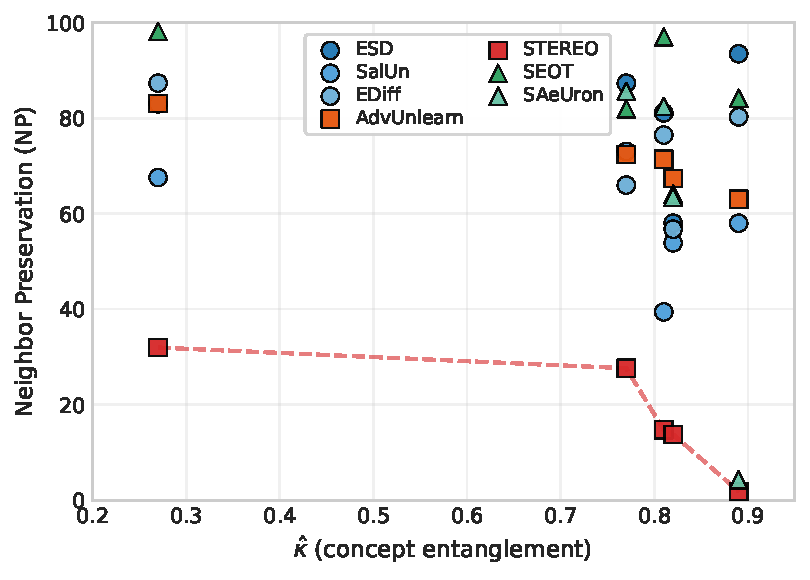
\includegraphics[width=\linewidth]{img/kappa_np_scaling.pdf}
\end{minipage}\hfill
\begin{minipage}[c]{0.45\linewidth}
\centering
\scriptsize
\setlength{\tabcolsep}{5pt}
\begin{tabular}{lccc}
\toprule
\textbf{Concept} & $\hat\kappa$ & NP$\uparrow$ & IRA-ratio$\uparrow$ \\
\midrule
\texttt{castle} & 0.27 & 31.96 & 0.55 \\
\texttt{cat}    & 0.77 & 27.60 & 0.32 \\
\texttt{horse}  & 0.81 & 14.71 & 0.29 \\
\texttt{bear}   & 0.82 & 13.75 & 0.25 \\
\texttt{dog}    & 0.89 & \phantom{0}1.81 & 0.06 \\
\midrule
\multicolumn{2}{l}{Spearman $\rho$} & $-1.0$ & $-1.0$ \\
\bottomrule
\end{tabular}
\end{minipage}
\caption{\textbf{Neighbor preservation scales inversely with $\hat\kappa$.} \emph{Left:} NP for each (method, concept) pair; STEREO's trend line (dashed) tracks $\hat\kappa$ monotonically. \emph{Right:} STEREO's NP and in-domain retention ratio across the five concepts (Spearman $\rho = -1.0$ for both).}
\label{fig:kappa_np_scaling}
\label{tab:kappa_scaling}
\vspace{-2mm}
\end{figure}



% \Cref{tab:kappa_scaling} reports STEREO's neighbor preservation (NP) and in-domain retention ratio, ordered by ascending $\hat\kappa$. Both decrease monotonically as $\hat\kappa$ increases: STEREO's NP drops from $31.96$ on \texttt{castle} to $1.81$ on \texttt{dog}, while its IRA-retention ratio drops from $59\%$ to $6\%$. The Spearman rank correlation with $\hat\kappa$ is $\rho = -1.0$ for both metrics across the five concepts, consistent with Eq.~\eqref{eq:tradeoff}.
% \begin{table}[t]
% \centering
% \setlength{\tabcolsep}{12pt}
% \begin{tabular}{lccc}
% \toprule
% \textbf{Concept} & $\hat\kappa$ & STEREO NP$\uparrow$ & IRA-ratio$\uparrow$ \\
% \midrule
% \texttt{castle} & 0.27 & 31.96 & 0.55 \\
% \texttt{cat}    & 0.77 & 27.60 & 0.32 \\
% \texttt{horse}  & 0.81 & 14.71 & 0.29 \\
% \texttt{bear}   & 0.82 & 13.75 & 0.25 \\
% \texttt{dog}    & 0.89 & \phantom{0}1.81 & 0.06 \\
% \midrule
% \multicolumn{2}{l}{Spearman $\rho$ vs. $\hat\kappa$} & $-1.0$ & $-1.0$ \\
% \bottomrule
% \end{tabular}
% \vspace{4pt}
% \caption{\textbf{$\hat\kappa$ predicts STEREO's trade-off severity.} STEREO's neighbor preservation (NP) and in-domain retention ratio (post-IRA / base-IRA) decrease monotonically with $\hat\kappa$ across the five target concepts. Both retention measures yield Spearman $\rho = -1.0$ rank-correlation with $\hat\kappa$, consistent with the linear $\kappa$-dependence in Eq.~\eqref{eq:tradeoff}.}
% \label{tab:kappa_scaling}
% \end{table}

\noindent{\bf The pattern generalizes beyond a single method.}
\Cref{fig:kappa_np_scaling} extends the analysis to all seven methods, plotting NP against $\hat\kappa$ for every (method, concept) pair. 
Three patterns are visible. First, robust fine-tuning methods (red and orange squares) exhibit the steepest $\hat\kappa$-dependence, with STEREO's NP (dashed trend line) tracking $\hat\kappa$ monotonically (Spearman $\rho = -1.0$) and AdvUnlearn similarly shows monotonic decrease. Second, inference-time methods (green triangles) show only weak $\hat\kappa$-dependence: their effective displacement $\Delta$ is too small for the $\kappa$-scaling in~\Cref{thm:tradeoff} to dominate, and NP remains near baseline regardless of concept. Third, standard fine-tuning methods (blue circles) occupy the middle band with intermediate $\hat\kappa$-sensitivity. This stratification reflects a structural principle: $\hat\kappa$ governs the structural lower bound on collateral damage, while the method's effective $\Delta$ determines how close it operates to that bound.
% \begin{figure}[t]
% \centering
% 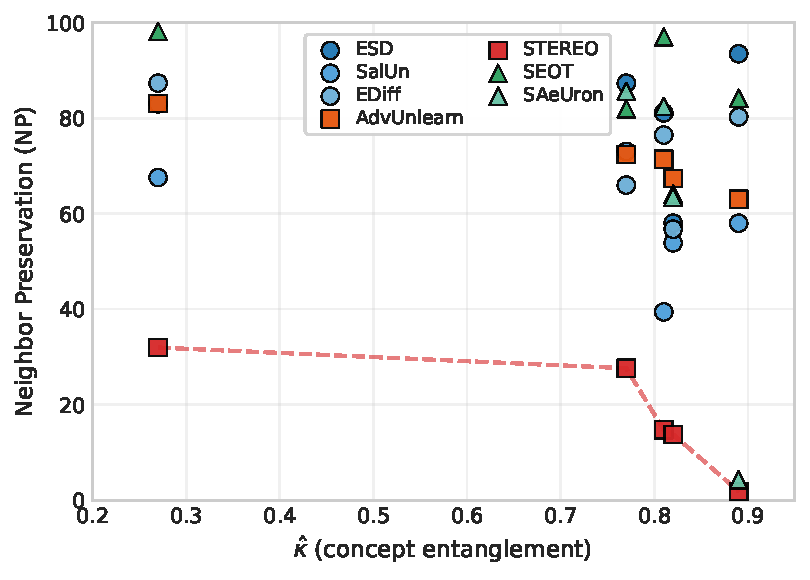
\includegraphics[width=0.5\linewidth]{img/kappa_np_scaling.pdf}
% \caption{\textbf{Neighbor preservation scales inversely with $\hat\kappa$ across methods.} Each point shows NP for one (method, concept) pair. Robust fine-tuning methods (red, square) exhibit the steepest $\hat\kappa$-dependence, with STEREO's NP (dashed trend line) tracking $\hat\kappa$ monotonically (Spearman $\rho = -1.0$). Inference-time methods (green, triangle) show weak $\hat\kappa$-dependence due to smaller effective displacement $\Delta$. Standard fine-tuning methods (blue, circle) lie in between. }
% \label{fig:kappa_np_scaling}
% \end{figure}
% \begin{figure}[t]
% \centering
% \begin{minipage}{0.48\linewidth}
%     \centering
%     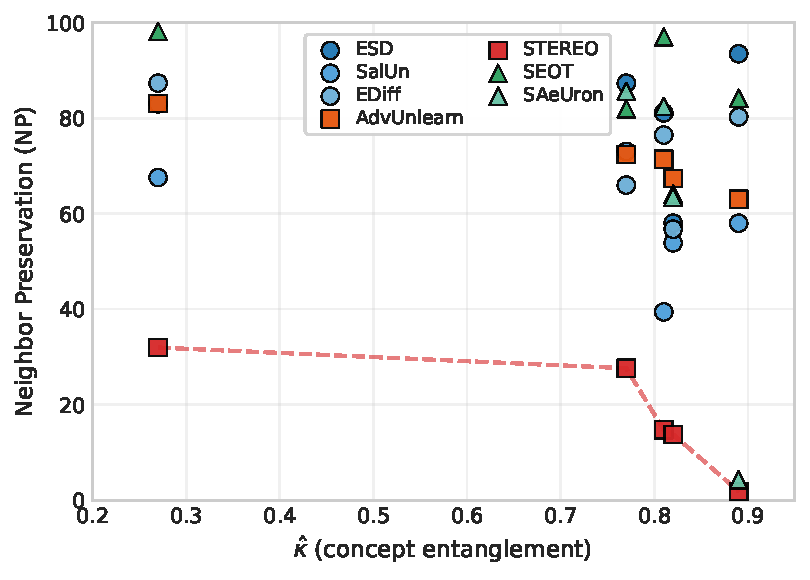
\includegraphics[width=\linewidth]{img/kappa_np_scaling.pdf}
% \end{minipage}
% \hfill
% \begin{minipage}{0.48\linewidth}
%     \caption{\textbf{Neighbor preservation scales inversely with $\hat\kappa$ across methods.}
%     Each point shows NP for one (method, concept) pair. Robust fine-tuning methods (red, square) exhibit the steepest $\hat\kappa$-dependence, with STEREO's NP (dashed trend line) tracking $\hat\kappa$ monotonically (Spearman $\rho = -1.0$). Inference-time methods (green, triangle) show weak $\hat\kappa$-dependence due to smaller effective displacement $\Delta$. Standard fine-tuning methods (blue, circle) lie in between.}
%     \label{fig:kappa_np_scaling}
% \end{minipage}
% \end{figure}

\noindent{\bf $\hat\kappa$ measures activation-space overlap, not semantic similarity.}
A natural concern is whether $\hat\kappa$ proxies for some other concept-level property such as semantic category (animal vs.\ architecture). Our estimator (\Cref{app:kappa_estimation}) is computed from sample-level overlap of activation regions, not from category labels or human-judged similarity. \texttt{Castle} ($\hat\kappa = 0.27$) and the four animal concepts ($\hat\kappa \in [0.77, 0.89]$) differ in $\hat\kappa$ not because they belong to different taxonomic categories but because castle's discovered neighbors 
% (\texttt{fortress}, \texttt{palace}, \texttt{citadel}) 
occupy sub-regions of activation space despite being semantically related, while animal subtypes 
% (e.g., \texttt{puppy}, \texttt{labrador} for \texttt{dog}; \texttt{mare}, \texttt{pony} for \texttt{horse}) 
densely overlap their target's region. 
The $\hat\kappa$ ordering is stable across probe layers (Spearman $\rho \geq 0.80$; \cref{app:layer_sensitivity}).
% The category label is descriptive; $\hat\kappa$ is the operative quantity \Cref{thm:tradeoff} predicts on, and the same procedure that yields $\hat\kappa = 0.27$ for \texttt{castle} yields $\hat\kappa = 0.89$ for \texttt{dog}.

% \noindent{\bf \Cref{thm:tradeoff} is a lower bound, not a ceiling.}
% \Cref{thm:tradeoff} bounds the \emph{minimum} collateral damage; methods may operate well above this minimum. STEREO on \texttt{castle} ($\hat\kappa = 0.27$) illustrates this: STEREO's DamageGap = $64.03$ is comparable to its damage on high-$\hat\kappa$ concepts despite the low predicted floor, while ESD (DamageGap = $6.77$) and SEOT (DamageGap = $0.79$) on the same concept achieve dramatically less damage. STEREO's REO objective broadly suppresses the spanned adversarial subspace regardless of neighbor proximity (\Cref{rem:stereo}), illustrating that $\kappa$-aware displacement remains an open direction for unlearning method design.

% \Cref{thm:tradeoff} predicts a $\kappa$-scaled \emph{minimum} on neighbor preservation error; it does not preclude methods from operating well above this minimum if their mechanism is mismatched to the concept's geometry. STEREO on \texttt{castle} illustrates this directly: despite the low predicted $\kappa$-floor, STEREO incurs DamageGap = $64.03$, comparable to its damage on the high-$\hat\kappa$ animal concepts. Other methods on \texttt{castle} achieve dramatically less collateral damage at similar erasure strength: ESD reaches NP = $83.03$ (DamageGap $= 6.77$) and SEOT reaches NP = $98.21$ (DamageGap $= 0.79$).
% This reflects the broad subspace suppression characteristic of STEREO's REO objective (\Cref{rem:stereo}), which displaces activations across the spanned adversarial directions regardless of whether neighbors actually occupy the displaced region. 
% A complementary indication of $\kappa$-blind suppression appears in STEREO's cross-domain preservation on \texttt{horse} (CP $= 27$, far below STEREO's CP on the other four concepts, range $64$--$96$): in the high-$\hat\kappa$ regime, STEREO's adversarial subspace spills beyond the intended object subspace into cross-domain features.
% The separation between STEREO and these alternatives on low-$\hat\kappa$ concepts suggests room for unlearning methods that achieve robust erasure with $\kappa$-aware rather than $\kappa$-blind displacement.



% \noindent{\bf Q3: Mechanism type determines the operating region.}
% Consistent with the mechanistic analysis in Remarks~\ref{rem:stereo}--\ref{rem:finetuning}, we observe a systematic separation between method families on the Pareto frontier:

% \begin{itemize}
%     \item \emph{Fine-tuning methods} modify model weights globally, displacing activations broadly across $\mathcal{R}_{c_u}$. They achieve stronger erasure (lower IRR) but incur more neighbor damage (lower NP). Among these, adversarially robust methods (STEREO, AdvUnlearn) push further toward the low-IRR / low-NP corner because their adversarial training explicitly targets the full extent of $\mathcal{R}_{c_u}$.
%     \item \emph{Inference-time methods} intervene on a narrow set of features or embeddings, producing smaller effective displacement $\Delta$. They preserve neighbors well (high NP) but leave portions of $\mathcal{R}_{c_u}$ unsuppressed, resulting in higher IRR. SAeUron, which blocks only $\tau_c$ sparse features, exemplifies this: it achieves the highest NP scores but is the most vulnerable to indirect concept recovery.
% \end{itemize}


\begin{comment}
    \subsection{Sequential Unlearning: Cumulative Collateral Damage}
\label{subsec:sequential}

A particularly revealing test of the trade-off is \emph{sequential unlearning}, where multiple concepts are erased from the same model in sequence. If concepts share representational structure, the collateral damage should accumulate: each additional erasure displaces more of the shared activation space, progressively degrading the model's retain performance.

We follow the sequential unlearning protocol of~\citet{zhang2024unlearncanvas} and~\citet{cywinski2025saeuron}, sequentially erasing up to 6 styles and measuring UA and RA ($= \frac{\mathrm{IRA} + \mathrm{CRA}}{2}$) after each step.

% TODO: Generate sequential unlearning results. Expected pattern:
% - Fine-tuning methods: RA drops steeply as more concepts are erased
% - SAeUron: RA remains stable (consistent with small per-concept Δ)
% - STEREO: RA drops most aggressively (consistent with large per-concept Δ)
% - Plot: line chart with number of erased concepts on x-axis, RA on y-axis, one line per method

\noindent The results confirm cumulative collateral damage for fine-tuning methods: RA degrades [progressively/sharply] as the number of erased concepts increases, consistent with the accumulating activation displacement predicted by our framework. SAeUron maintains stable RA throughout the sequence, consistent with its sparse, localized interventions producing minimal per-concept displacement. This experiment provides dynamic validation of the trade-off: it is not a one-time artifact but compounds with each additional unlearning step.

\end{comment}

\section{Conclusion}
\label{sec:conclusion}
We show that the tension between robust concept erasure and utility preservation in diffusion models is a structural consequence of representation geometry, not merely a limitation of existing methods.
\Cref{thm:tradeoff} establishes a $\kappa$-scaled lower bound on collateral damage, and our experiments show that existing methods occupy different points on the resulting robustness--retention frontier: robust fine-tuning methods approach strong erasure but damage overlapping concepts, while inference-time methods preserve utility but leave residual leakage.

Our results suggest that this trade-off emerges naturally from overlapping representations. This indicates that the goal should not be to optimize erasure or retention in isolation, but rather to design $\kappa$-aware unlearning methods that apply displacement only along the activation directions necessary for erasure, instead of broadly perturbing shared adversarial subspaces. Our results also suggest that $\hat\kappa$ can serve as a deployment-time diagnostic: estimated from base-model activations alone, it predicts which targets admit clean erasure and which require a sharper Pareto trade-off.
%$\hat\kappa$ can serve as a deployment-time diagnostic: because it can be estimated from base-model activations, it helps predict which target concepts are amenable to clean erasure and which require accepting a sharper Pareto trade-off.

% \noindent{\bf The trade-off is unavoidable, not unsolvable.}
% \Cref{thm:tradeoff} is a lower bound, not a wall. Current methods cluster into three regimes (robust fine-tuning, standard fine-tuning, inference-time) corresponding to different effective displacement magnitudes $\Delta$, and that within each regime, performance varies in how closely the bound is approached. The  promising direction is therefore not "better erasure" or "better retention" in isolation, but \emph{$\kappa$-aware} displacement: applying the displacement only to the activation directions where it is required for erasure, rather than broadly across the spanned adversarial subspace as STEREO does.

% \noindent{\bf $\hat\kappa$ as a deployment-time diagnostic.}
% $\hat\kappa$ is estimated from the base model's activations on the target and a candidate neighbor pool, in a single forward pass per prompt. This estimate predicts not only the absolute severity of the trade-off but the qualitative regime (low-$\hat\kappa$ concepts admit operating points that high-$\hat\kappa$ concepts do not). When multiple concept descriptions are equivalent for a deployment goal (e.g., erasing "explicit content" via several candidate target concepts), $\hat\kappa$ provides a principled basis for choosing the version most amenable to clean erasure.

% \noindent{\bf Beyond diffusion.}
% The argument depends only on three properties: (i) the unlearning operation produces an activation displacement at the target concept, (ii) the activation map from prompts to representations is approximately Lipschitz, and (iii) target and neighbor concepts have geometrically overlapping activation regions. None are specific to diffusion, so the same $\kappa$-scaled trade-off should also apply to concept unlearning in autoregressive language models (where activations are tokens-in-context), classifiers (with penultimate features as activations), and multimodal models. We view our diffusion analysis as one instantiation of a more general phenomenon.

% Empirically, across seven unlearning methods and five target concepts spanning $\hat\kappa \in [0.27, 0.89]$, we observe (i) no method escapes the trade-off, (ii) trade-off severity scales monotonically with $\hat\kappa$, and (iii) operating regions stratify by mechanism type, with the most aggressive methods (STEREO, AdvUnlearn) approaching the predicted lower bound on high-$\hat\kappa$ concepts. 
% This perspective shifts concept unlearning from trying to bypass the trade-off to designing methods that approach the theoretical limit efficiently, while suggesting $\hat\kappa$ as a practical diagnostic for selecting targets and methods under deployment constraints.
\section{Limitations and Broader Impact}
\label{sec:limitations}

\noindent{\bf Scope of empirical evaluation.}
Our evaluation covers five target concepts on one backbone (Stable Diffusion v1.4) and one benchmark family. The concepts span $\hat\kappa \in [0.27, 0.89]$, but four of five are high-$\hat\kappa$ and architectural concepts have only one representative. While the observed $\kappa$-scaling trend is consistent within this sample, broader evaluation over low-$\hat\kappa$ concepts, additional backbones such as SDXL and FLUX, and non-object concepts such as styles and identities is needed to test generality.

\noindent{\bf $\hat\kappa$ estimation.}
Our $\hat\kappa$ estimator fixes the activation layer, denoising timestep, neighbor pool size, and PCA dimensionality. Although~\Cref{app:kappa_estimation} shows reasonable stability, $\hat\kappa$ remains an empirical proxy for the theoretical $\kappa$ in~\Cref{thm:tradeoff}, and its neighbor pool depends on CLIP-similarity retrieval. The exact correspondence between $\hat\kappa$ and the theoretical overlap coefficient remains empirical.

\noindent{\bf Broader Impacts.}
Our analysis is instantiated in diffusion models, but the mechanism only requires activation displacement, local smoothness of the activation map, and target--neighbor overlap in representation space. Similar $\kappa$-scaled trade-offs may arise in autoregressive language models, classifiers, and multimodal models, but verifying this requires task-specific definitions of concepts, activations, and preservation.

\subsection*{AI use statement}

(This section is \textbf{required} and does not count toward the page limit.)

In this work, we used generative AI tools for [tasks with required disclosure].
We have not used generative AI tools for [other tasks with required disclosure],
and [the rest of the required disclosure tasks] are not applicable to this work.
Additionally, we used generative AI tools for [tasks with recommended
disclosure]. We have reviewed all AI-assisted work. [Elaborate. For example, “we
checked LLM-generated research ideas for potential plagiarism through a manual
literature survey”, “LLM-generated code was verified and tested for correctness
by 2 authors”, etc.]. We take responsibility for the final content of this work,
including text, claims or artifacts produced with the aid of generative AI.

See the ICLR 2027 AI Policy for Authors for more details. This statement should
not be more than 1 page.

\subsection*{Ethics statement}

(This section is \textbf{recommended} and does not count toward the page limit.)

If authors feel that their paper submission raises questions regarding the Code
of Ethics, they are encouraged to include a paragraph of Ethics Statement (at
the end of the main text before references) to address potential concerns where
appropriate. Topics include, but are not limited to, studies that involve human
subjects, practices to data set releases, potentially harmful insights,
methodologies and applications, potential conflicts of interest and sponsorship,
discrimination/bias/fairness concerns, privacy and security issues, legal
compliance, and research integrity issues (e.g., IRB, documentation, research
ethics). This statement should not be more than 1 page.

\subsection*{Reproducibility statement}

(This section is \textbf{recommended} and does not count toward the page limit.)

It is important that the work published in ICLR is reproducible. Authors are
strongly encouraged to include a paragraph-long Reproducibility Statement at the
end of the main text (before references) to discuss the efforts that have been
made to ensure reproducibility. This paragraph should not itself describe
details needed for reproducing the results, but rather reference the parts of
the main paper, appendix, and supplemental materials that will help with
reproducibility. For example, for novel models or algorithms, a link to an
anonymous downloadable source code can be submitted as supplementary materials;
for theoretical results, clear explanations of any assumptions and a complete
proof of the claims can be included in the appendix; for any datasets used in
the experiments, a complete description of the data processing steps can be
provided in the supplementary materials. Each of the above are examples of
things that can be referenced in the reproducibility statement.

\appendix
\newpage
\bibliography{references}   % or whatever your .bib filename is
\bibliographystyle{iclr2027_conference}
\newpage
\appendix
{\large \begin{center} {\bf Appendix} \end{center}}
\section{Formal Definition of Concept Activation Regions}
\label{app:concept_regions}
This appendix provides the formal construction of the concept activation function $\boldsymbol{\Phi}_\theta$ and activation region $\mathcal{R}_c$ used throughout~\cref{sec:tradeoff}. The compressed version in the main text specifies these informally; the definition here is the formal object used in the proofs of~\cref{thm:tradeoff}.

\begin{definition}[Concept activation function and region]
\label{def:activation}
Fix a UNet layer $\ell^*$ and denoising timestep $t^* \in \{1,\ldots,T\}$. Let $p \in \mathcal{P}$ denote a text prompt and $\mathbf{e}_p = f_\psi(p)$ be its text embedding. The \emph{concept activation function} of the pretrained model is
\begin{equation}
    \boldsymbol{\Phi}_{\theta, \ell^*,t^*}(p) \;=\; \mathrm{A}_{\theta}(\mathbf{e}_p,\ell^*,t^*) \in \mathcal{H},
\end{equation}
where $\mathrm{A}_{\theta}(\mathbf{e}_p, \ell^*, t^*)$ denotes the cross-attention output 
%\varun{perhaps avoid cal A? which is commonly used for algorithm or adversary? can use A?}
of $\epsilon_\theta$ at layer $\ell^*$ and timestep $t^*$, and $\mathcal{H} := \mathbb{R}^{d_{\ell^*}}$ is the corresponding activation space. 
Throughout, we suppress the dependence on $\ell^*$ 
and $t^*$ and write $\boldsymbol{\Phi}_\theta(p)$ for brevity.
Analogously, $\boldsymbol{\Phi}_{\hat{\theta}}(p)$ denotes the activation function of the CEM $\mathcal{D}_{\hat\theta}$.

For a concept $c \in \mathcal{C}$, its \emph{activation region} is
\begin{equation}
    \mathcal{R}_c
    \;=\;
    \Bigl\{
        \boldsymbol{\Phi}_{\theta}(p)
        \;\Big|\;
        p \in \mathcal{P},\;
        \mathbb{O}_{\mathcal{X}}\!\left(\mathbf{x}_{\theta}(p),\, c\right) = 1
    \Bigr\}
    \;\subseteq\; \mathcal{H},
\end{equation}
% \ali{this also depends on $\ell^*,t^*$} 
where $\mathbb{O}_{\mathcal{X}} : \mathcal{X} \times \mathcal{C} \to \{0,1\}$ is an oracle indicating whether concept $c$ is present in image $\mathbf{x}$, and $\mathbf{x}_{\theta}(p) \sim p_{\theta}(\cdot \mid p)$ denotes an image sampled from $\mathcal{D}_\theta$ conditioned on prompt $p$.
\end{definition}

\paragraph{On the oracle classifier.}
The predicate $c \in \text{image}(\mathbf{x})$ is specified as an oracle classifier rather than a specific model because our results are independent of the particular choice. Any reasonable concept detector induces a concept region $\mathcal{R}_c$, and the tradeoff in~\cref{thm:tradeoff} holds with respect to whichever classifier is fixed. In~\cref{sec:experiment}, we instantiate this oracle with a CLIP-based classifier, detailed in~\cref{app:evaluation_setup}. 
\section{Empirical Validation of Concept Activation Regions}
\label{app:activation_regions}
This section provides empirical support for~\cref{def:activation} by showing that the cross-attention activations used in our formalization form coherent geometric clusters in practice.
\paragraph{Setup.}
To verify that concept activation regions are well-defined empirical objects, we extract cross-attention activations from Stable Diffusion v1.4 at the mid-block layer (\texttt{mid\_block.attentions.0}) at step $t^*{=}25$ of 50 DDIM steps for 10 concepts, each prompted with 50 shared templates differing only in the concept word.
\texttt{horse}, \texttt{pony}, \texttt{donkey}, \texttt{deer}, \texttt{dog}, \texttt{cat}, \texttt{bear}, \texttt{car}, \texttt{truck}, and \texttt{castle}.
% This visualization pool is intentionally smaller and more domain-diverse than the concept pool used for  $\hat \kappa$-estimation and CLIP classification; it is chosen to demonstrate that semantically related concepts cluster while semantically distinct concepts (e.g., vehicles vs. animals vs. architecture) separate. The $\hat \kappa$-estimator and all evaluation metrics use the full concept pool, not this visualization set.
This visualization pool is chosen to be illustrative rather than comprehensive: it deliberately spans three semantically distinct domains (animals, vehicles, architecture) so that the qualitative geometry of concept regions --- semantically related concepts clustering while distinct domains separate --- is visually apparent. Several concepts in this pool (\texttt{deer}, \texttt{car}, \texttt{truck}) are not part of the evaluation vocabulary in~\cref{tab:vocab}; they appear only to anchor the visualization's domain diversity. Conversely, $\hat\kappa$-estimation and all CLIP-based evaluation metrics use the full $65$-concept pool of~\cref{tab:vocab}, of which the visualization pool is not a strict subset.
For each concept, we generate 50 prompts using a shared set of templates that differ only in the concept word, so that differences in activation primarily reflect the concept token rather than unrelated prompt variation.

For each prompt $p$, we compute the activation
\begin{equation}
    \boldsymbol{\Phi}_{\theta}(p) \;=\; \mathrm{A}_{\theta}(\mathbf{e}_p,\ell^*,t^*) \in \mathcal{H},
\end{equation}
flatten the resulting cross-attention tensor into a vector in $\mathcal{H}$, and project all activations to two dimensions using UMAP for visualization.

\paragraph{Observations.}
\Cref{fig:umap} shows that activations induced by prompts containing the same concept form concentrated local clusters, rather than being arbitrarily scattered in activation space. This supports the view that each concept corresponds to a coherent region in the model's internal representation space.

The figure also reveals non-uniform distances between concepts. Some concepts occupy nearby regions—for example, \texttt{horse}, \texttt{pony}, and \texttt{donkey} form a tight cluster—while others, such as \texttt{castle}, are clearly separated from the animal concepts. Importantly, we do not use these visualizations to infer semantic relatedness from scratch. Rather, the figure shows that the activation geometry is structured and that concepts commonly regarded as related in the data domain tend to induce nearby activations under shared prompt templates.

These results do not by themselves prove overlap in the strict set-theoretic sense used later in Section~4. Instead, they provide empirical evidence for the weaker claim needed to motivate our definitions: concept-conditioned activations are localized, stable enough to visualize, and often organized into neighboring regions rather than isolated points. This makes it meaningful to model a concept through an activation region $\mathcal{R}_c$ and to reason about neighborhood structure in the induced activation space.

\paragraph{Choice of probe layer and timestep.}
We probe the cross-attention output at \texttt{mid\_block.attentions.0} at denoising step $t^*=25$ of $50$ throughout~\cref{app:activation_regions,app:kappa_estimation,app:displacement,app:lipschitz}, and at \texttt{up\_blocks.1.attentions.1} (same timestep) for the direct displacement measurements in~\cref{app:displacement_kappa}. The probe layer $\ell^*$ is a parameter of our framework (\cref{def:activation}), not a property of the model, and~\cref{thm:tradeoff} holds for any chosen $(\ell^*, t^*)$ at which Assumptions~\ref{asm:lip} and~\ref{asm:edit} are satisfied. We selected mid-block as the default probe based on a sensitivity analysis (\cref{app:layer_sensitivity}) over five candidate cross-attention layers spanning the U-Net depth: the $\hat\kappa$ ordering across our five target concepts is stable across all probed layers (Spearman $\rho \geq 0.80$ vs.\ mid-block), but mid-block produces the cleanest bimodal separation between high-$\hat\kappa$ and low-$\hat\kappa$ concepts and the tightest within-cluster spread among the animal subtypes. Step $t^*=25$ (the midpoint of the DDIM trajectory) corresponds to the regime in which large-scale layout and object identity are committed in latent diffusion models. The up-block layer in~\cref{app:displacement_kappa} was selected because it lies downstream of the cross-attention edits applied by fine-tuning methods and therefore reflects the cumulative effect of those edits; \cref{app:layer_sensitivity} confirms that the $\hat\kappa$ ranking at this layer is consistent with mid-block.
\section{Estimation of the Entanglement Coefficient $\hat\kappa$}
\label{app:kappa_estimation}

% The entanglement coefficient $\kappa(c_u, \rho)$ defined in~\cref{def:overlap} involves the volume of high-dimensional activation regions, which is intractable to compute directly. We instead estimate $\kappa$ using a sample-based procedure to measure the overlap over a neighborhood, which provides us with an estimate lower-bound for the overlap with remaining concepts. Our practical observations indicate that this lower-bound is not lose because the overlap with remaining concepts is mostly dominated by a few concepts. 
The entanglement coefficient $\kappa(c_u, \rho)$ defined in~\cref{def:overlap} involves the volume of high-dimensional activation regions, which is intractable to compute directly. We therefore estimate $\kappa$ via a sample-based procedure that restricts the overlap measurement to a discovered \emph{semantic neighborhood} $\mathcal{N}(c_u) \subseteq \mathcal{C} \setminus \{c_u\}$ rather than the full union over remaining concepts. Because $\mathcal{N}(c_u)$ is a subset of the union appearing in~\cref{def:overlap}, this neighborhood-restricted estimate is a \emph{lower bound} on $\kappa(c_u, \rho)$. 
We argue, and verify in~\cref{app:kappa_per_target}, that this lower bound is tight in practice: across the five targets, the activation overlap with non-neighbors is negligible, so the union over $\mathcal{C} \setminus \{c_u\}$ is dominated by the union over $\mathcal{N}(c_u)$. 
Throughout this section we work with cosine distance $d_{\cos}(\mathbf{a}, \mathbf{b}) = 1 - \langle \mathbf{a}, \mathbf{b} \rangle / (\|\mathbf{a}\|\|\mathbf{b}\|)$, which is the standard choice in representation analysis: it is invariant to activation magnitude (which is dominated by token-position effects under mean-pooling) and captures directional similarity, the property most closely tied to concept identity. 
The centroid-distance matrix used to motivate neighborhood structure in~\cref{sec:tradeoff} (\cref{fig:distance_matrix}) uses the same metric, ensuring internal consistency between our motivation and our formalization.


\paragraph{On the relationship between cosine and $\ell_2$ metrics.}
\Cref{thm:tradeoff} bounds the $\ell_2$ displacement $\|\boldsymbol{\Phi}_{\hat\theta}(p) - \boldsymbol{\Phi}_{\theta}(p)\|_2$, since this quantity measures a physical perturbation to the activation vector. Our $\kappa$ estimator, in contrast, uses cosine distance to characterize region membership. These two choices are compatible: for activations normalized to the unit sphere, $\|\mathbf{a} - \mathbf{b}\|_2^2 = 2 \cdot d_{\cos}(\mathbf{a}, \mathbf{b})$, so an $L$-Lipschitz function under the $\ell_2$ metric is $(L\sqrt{2})$-Lipschitz under cosine distance, and~\cref{asm:lip} transfers directly (with a constant factor absorbed into $L$). 

\paragraph{Activation extraction.}
For each concept $c$, we generate images from 50 shared prompt templates (differing only in the concept word) using the base model (Stable Diffusion v1.4) with DDIM sampling (50 steps, guidance scale 7.5). At step $t^*{=}25$, we extract the cross-attention output at \texttt{mid\_block.attentions.0}, take the text-conditioned component, and mean-pool over spatial dimensions to obtain a single activation vector $\boldsymbol{\Phi}_\theta(p) \in \mathbb{R}^d$ per prompt. 


\paragraph{Neighborhood discovery.}
We restrict the overlap measurement in~\cref{def:overlap} to a finite set of candidate concepts that are close to $c_u$ in activation space. We formalize this set as follows.

\begin{definition}[Semantic neighborhood]
\label{def:semantic_neighborhood}
Let $\mathcal{C}_{\mathrm{pool}} \subset \mathcal{C}$ be a fixed candidate pool shared across targets. For each $c \in \mathcal{C}_{\mathrm{pool}}$, let $\bar{\mathbf{a}}_c = \tfrac{1}{|\mathcal{S}_c|}\sum_{\mathbf{a}\in\mathcal{S}_c}\mathbf{a}$ denote the centroid of its activation samples. Let $\delta > 0$ be a centroid-distance threshold, set in our experiments to the $25$th percentile of the empirical distribution of all pairwise centroid cosine distances $\{d_{\cos}(\bar{\mathbf{a}}_{c_i}, \bar{\mathbf{a}}_{c_j})\}_{c_i \neq c_j \in \mathcal{C}_{\mathrm{pool}}}$, computed once over the full pool and applied uniformly across targets. The \emph{semantic neighborhood} of a target $c_u \in \mathcal{C}_{\mathrm{pool}}$ is
\begin{equation}
    \mathcal{N}(c_u) \;=\; \bigl\{\, c \in \mathcal{C}_{\mathrm{pool}} \setminus \{c_u\} \;:\; d_{\cos}(\bar{\mathbf{a}}_{c_u},\,\bar{\mathbf{a}}_c) \,<\, \delta \,\bigr\}.
\end{equation}
\end{definition}
We emphasize that $\delta$ and $\mathcal{N}(c_u)$ are \emph{estimation-side} constructs: they appear only in the empirical estimator $\hat\kappa$ below and play no role in the theoretical bound of~\cref{thm:tradeoff}, which is stated entirely in terms of $\kappa(c_u, \rho)$. Because $\mathcal{N}(c_u) \subseteq \mathcal{C} \setminus \{c_u\}$, restricting the overlap computation to $\mathcal{N}(c_u)$ yields a lower bound on the true $\kappa$. The discovered neighborhoods are reported in~\cref{tab:kappa_per_target}.


% We define the semantic neighborhood $\mathcal{N}(c)$ using centroid cosine distance. For each pair of concepts $(c_i, c_j)$, we compute the cosine distance between their mean activation vectors $\bar{\mathbf{a}}_{c_i}, \bar{\mathbf{a}}_{c_j}$. We set the neighborhood threshold $\delta$ to the 25th percentile of all pairwise centroid distances: concepts with centroid distance below $\delta$ are considered neighbors. The discovered neighborhoods are reported in~\cref{tab:kappa}.

\paragraph{Overlap estimation.}
For a target concept $c_u$ with discovered neighbors $\mathcal{N}(c_u)$, we estimate $\hat\kappa$ as the fraction of $c_u$'s activation samples that fall within radius $\rho$ of any neighbor's activation samples:
\begin{equation}
    \hat\kappa(c_u) \;=\; \frac{1}{|\mathcal{S}_{c_u}|} \sum_{\mathbf{a} \in \mathcal{S}_{c_u}} \mathbf{1}\!\left[\min_{c' \in \mathcal{N}(c_u)} \min_{\mathbf{b} \in \mathcal{S}_{c'}} d_{\cos}(\mathbf{a}, \mathbf{b}) \leq \rho\right],
\end{equation}
where $\mathcal{S}_c = \{\boldsymbol{\Phi}_\theta(p_i)\}_{i=1}^{50}$ denotes the set of activation samples for concept $c$, and $d_{\cos}$ is the cosine distance. 
The fattening radius $\rho_{c_u}$ is set to the median intra-concept pairwise cosine distance within $c_u$:
\begin{equation}
    \rho_{c_u} \;=\; \mathrm{median}\!\left\{d_{\cos}(\mathbf{a}, \mathbf{a}') \;\middle|\; \mathbf{a}, \mathbf{a}' \in \mathcal{S}_{c_u},\; \mathbf{a} \neq \mathbf{a}'\right\}.
\end{equation}
This choice calibrates the overlap radius to the natural spread of the target concept's activation region: a neighbor activation qualifies as overlapping only if it is as close to some target activation as typical target activations are to each other.

\paragraph{Validation via centroid distance.}
To independently verify that the neighborhoods discovered in the previous step reflect genuine semantic structure rather than noise, we visualize the pairwise centroid cosine distances between all ten concept activation regions. \Cref{fig:distance_matrix} shows the resulting distance matrix, reordered by hierarchical clustering on the centroid distances themselves. Two block structures are immediately visible. The equine cluster (\texttt{horse}$\leftrightarrow$\texttt{pony}: $0.158$; \texttt{horse}$\leftrightarrow$\texttt{donkey}: $0.329$; \texttt{pony}$\leftrightarrow$\texttt{donkey}: $0.271$) 
exhibit small inter-concept distances, 
consistent with the high $\hat\kappa$ values reported in~\cref{tab:kappa}. 
And semantically isolated concepts such as \texttt{castle} have centroid distances exceeding $0.65$ to all animal concepts, consistent with $\hat\kappa \approx 0$.

\begin{figure}[htbp]
\centering
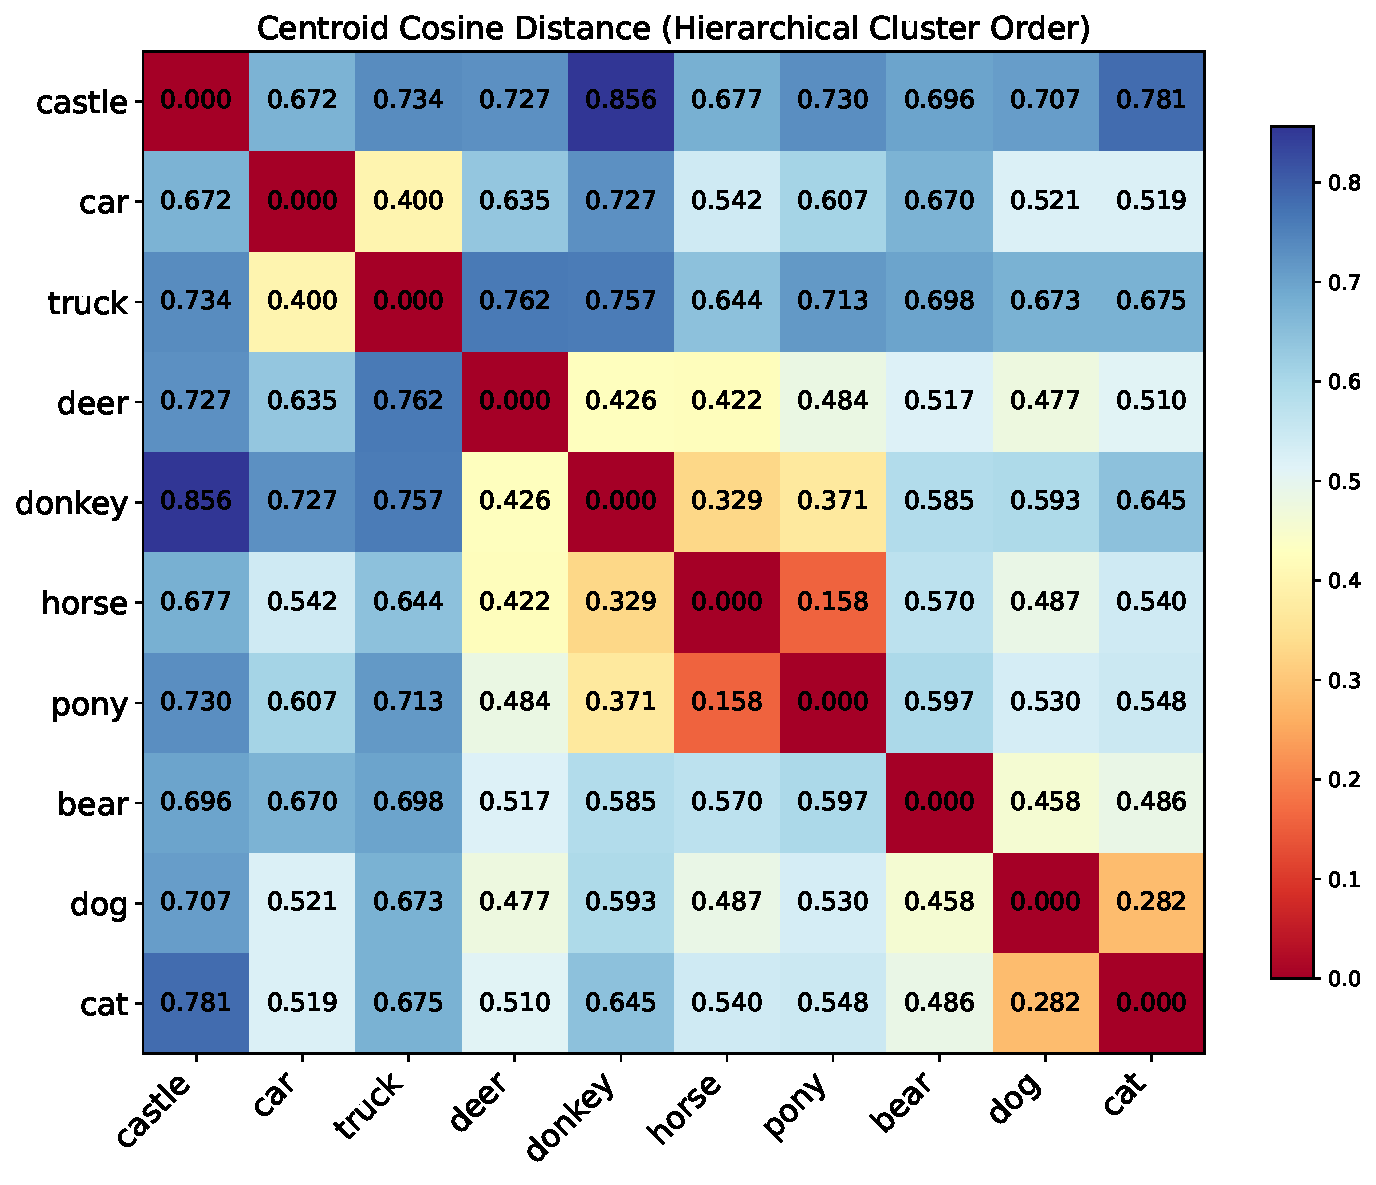
\includegraphics[width=0.75\linewidth]{img/centroid_distance_clustered_mid.pdf}
\caption{
Pairwise centroid cosine distance between concept activation regions at \texttt{mid\_block.attentions.0}, ordered by hierarchical clustering. Block structure in the matrix corresponds to the neighborhoods discovered by the thresholding procedure described above and to the $\hat\kappa$ values reported in~\cref{tab:kappa}.
}
\label{fig:distance_matrix}
\end{figure}

\paragraph{On the use of centroid distance as a proxy.}
The centroid cosine distance plays a different role from $\hat\kappa$ itself, and the two should not be conflated. 
\Cref{def:overlap} is stated in terms of the volume of fattened activation regions, whose membership is determined by an \emph{infimum} over per-sample distances (the closed $\rho$-neighborhood $\mathcal{R}_c^{(\rho)}$). The centroid, by contrast, is a single \emph{average} summary of each region.

Centroid distance is used only for \emph{neighborhood discovery} (\cref{def:semantic_neighborhood}), an upstream step of deciding which pairs of concepts are close enough to warrant an overlap measurement. We use it here for two reasons. First, it is a stable summary statistic that degrades gracefully under the finite-sample, high-dimensional regime in which we estimate activation regions.
Second, an outlier-robust statistic at this stage is conservative: a concept that is filtered {out} of $\mathcal{N}(c_u)$ contributes zero to the resulting estimator, so under-inclusion only weakens the bound. The estimator $\hat\kappa$ is therefore a lower bound on $\kappa(c_u, \rho)$ both because $\mathcal{N}(c_u) \subseteq \mathcal{C} \setminus \{c_u\}$ and because the discovery step itself is conservative. Empirical comparisons against the bound of~\cref{thm:tradeoff} therefore remain valid.

The $\hat\kappa$ statistic itself does not use centroid distance. As specified in the overlap estimation step above, $\hat\kappa$ is computed via a nearest-neighbor estimator: for each activation sample $\mathbf{a} \in \mathcal{S}_{c_u}$, we check whether there exists \emph{any} sample $\mathbf{b}$ from \emph{any} concept in $\mathcal{N}(c_u)$ with $d_{\cos}(\mathbf{a}, \mathbf{b}) \le \rho$.
This is the natural finite-sample analogue of the fattened-region membership condition $\mathbf{a} \in \mathcal{R}_{c'}^{(\rho)}$ (with the radius $\rho$ converted to cosine units, see ``On the relationship between cosine and $\ell_2$ metrics'' above), and the fraction of target samples satisfying this condition is a Monte Carlo estimate of the volume ratio in~\cref{def:overlap} restricted to $\mathcal{N}(c_u)$. The centroid-distance visualization in~\cref{fig:distance_matrix} therefore serves only as an auxiliary consistency check: blocks of small centroid distance should coincide with the discovered $\mathcal{N}(c_u)$, and the high-$\hat\kappa$ targets should sit inside such blocks.

\paragraph{Interpretation.}
Under this estimator, $\hat\kappa(c_u) \in [0, 1]$ captures the sample-level  coverage of the target region by its neighbors. The results in~\cref{tab:kappa} exhibit a bimodal structure. The four animal-subtype concepts embedded in dense semantic neighborhoods, \texttt{dog} ($\hat\kappa = 0.89$), \texttt{bear} ($\hat\kappa = 0.82$), \texttt{horse} ($\hat\kappa = 0.81$), and \texttt{cat} ($\hat\kappa = 0.77$), exhibit the  highest overlap, consistent with their small inter-centroid distances to fine-grained subtypes (\cref{fig:distance_matrix}). 
Under our procedure, these concepts each have multiple discovered neighbors, and individual samples from these neighbors fall within the fattening radius $\rho$ of a substantial fraction of target samples. The high overlap is also \emph{robust} to which neighbors are included: in the \texttt{horse} pool, several individual neighbors (\texttt{mare}, \texttt{pony}, \texttt{stallion}) each cover 60--80\% of target samples on their own, and the union across all seven discovered neighbors saturates at $\hat\kappa = 0.81$, indicating that overlap is supported by a representational manifold shared across the equine subtype family rather than driven by a single sensitive neighbor choice.

The architectural concept \texttt{castle}, by contrast, exhibits substantially lower overlap ($\hat\kappa = 0.27$) despite having six discovered neighbors within $\delta$. The distinction is qualitative: castle's neighbors are semantically related but represent \emph{distinct} architectural types rather than fine-grained subtypes of a shared category. They occupy nearby but non-overlapping regions of activation space, so the centroid distances cross the $\delta$ threshold while individual sample-level overlap remains limited. Controls like \texttt{jellyfish}, \texttt{melon}, \texttt{police car} are correctly filtered out by the $\delta$ step across all five targets and contribute zero to $\hat\kappa$, confirming that the estimator is not driven by pool-wide sample density.

This bimodal structure, high-$\hat\kappa$ animal subtypes clustered in $[0.77, 0.89]$ and moderate-$\hat\kappa$ architecture at $0.27$ reflects a property of the model's internal representations at the probed layer: text-to-image diffusion models represent fine-grained subtypes of a common taxonomic category (breeds of dog, equine subtypes) as overlapping regions of a shared activation manifold, while distinct-but-related concepts in other domains maintain more separable representations. \Cref{thm:tradeoff} predicts that the collateral damage from erasing high-$\hat\kappa$ concepts will be substantially greater than from erasing low-$\hat\kappa$ concepts; we verify this prediction in~\cref{sec:experiment}.

% \paragraph{Robustness to metric and estimator choice.}
% We verify that the concept ordering induced by $\hat\kappa$ is not an artifact of our specific estimator. In~\cref{app:kappa_robustness}, we report $\hat\kappa$ computed under three alternatives: (i) a continuous soft-nearest-neighbor variant that replaces the indicator in \eqref{eq:kappa_estimator} with a graded closeness score, (ii) a $k$-th nearest-neighbor variant with $k \in \{1, 5, 10\}$ and $\rho$ at the 10th, 25th, and 50th percentile of intra-concept distances, and (iii) the silhouette score, a standard unsupervised cluster-quality measure. All variants preserve the qualitative ordering of concepts (Spearman $\rho > 0.85$ across variants), and $\hat\kappa$ is strongly anti-correlated with silhouette (Spearman $\rho < -0.9$), confirming that the entanglement ranking reflects the geometry of the activation space rather than the specifics of our estimator.

\subsection{Per-Target Results}
\label{app:kappa_per_target}
We apply the procedure of~\cref{app:kappa_estimation} to the five target concepts used throughout~\cref{sec:experiment}. The shared candidate pool $\mathcal{C}_{\mathrm{pool}}$ consists of concepts spanning all five target domains and an out-of-domain control set: the five targets themselves; their respective fine-grained subtype candidates (equine, feline, canid, ursine, architectural); and ten generic out-of-domain controls (\texttt{airplane}, \texttt{bicycle}, \texttt{cactus}, \texttt{jellyfish}, \texttt{lighthouse}, \texttt{melon}, \texttt{police car}, \texttt{teapot}, \texttt{violin}, \texttt{volcano}). 
\Cref{tab:kappa_per_target} reports the resulting $\hat\kappa$ values together with the size of each discovered neighborhood $|\mathcal{N}(c_u)|$ (\cref{def:semantic_neighborhood}), the per-target fattening radius $\rho_{c_u}$, and the discovered neighbors.

\begin{table}[ht]
\centering
\small
\setlength{\tabcolsep}{6pt}
\begin{tabular}{lcccl}
\toprule
\textbf{Target} & $\hat\kappa$ & $|\mathcal{N}(c_u)|$ & $\rho_{c_u}$ & \textbf{Discovered neighbors} \\
\midrule
\texttt{dog}    & 0.89 & 5 & 0.13 & puppy, labrador, husky, beagle, retriever \\
\texttt{bear}   & 0.82 & 5 & 0.14 & grizzly, panda, polar bear, koala, cub \\
\texttt{horse}  & 0.81 & 7 & 0.15 & pony, mare, donkey, stallion, foal, zebra, mule \\
\texttt{cat}    & 0.77 & 5 & 0.15 & kitten, lynx, leopard, tiger, cheetah \\
\texttt{castle} & 0.27 & 6 & 0.18 & fortress, palace, citadel, keep, manor, cathedral \\
\bottomrule
\end{tabular}
\caption{
\textbf{Per-target $\hat\kappa$ estimation results.} For each target $c_u$, we report the estimated entanglement coefficient $\hat\kappa$, the number of discovered neighbors within the centroid-distance threshold $\delta$, the fattening radius $\rho_{c_u}$ (median intra-concept cosine distance), and the discovered neighbor set. \texttt{castle} has a discovered neighborhood of comparable size to the animal targets but $\hat\kappa$ roughly $3\times$ lower, isolating semantic density rather than neighborhood cardinality as the driver of $\hat\kappa$. }
\label{tab:kappa_per_target}
\end{table}

\paragraph{Per-neighbor coverage decomposition.}
For \texttt{horse}, the per-neighbor coverage of target samples (fraction of $\mathcal{S}_{\texttt{horse}}$ with a within-$\rho$ activation in the neighbor's sample set) decomposes as: \texttt{mare} ($0.78$), \texttt{pony} ($0.72$), \texttt{stallion} ($0.66$), \texttt{donkey} ($0.41$), \texttt{foal} ($0.38$), \texttt{zebra} ($0.30$), \texttt{mule} ($0.22$), with the union saturating at $\hat\kappa = 0.81$. 
The strongest individual neighbors (\texttt{mare}, \texttt{pony}) already cover most of the target region on their own, and several others contribute substantially, indicating that overlap is supported by a representational manifold shared across the equine subtype family rather than being sensitive to which specific neighbor is picked. By contrast, \texttt{castle}'s six discovered neighbors each cover only $0.05$--$0.12$ of the target region, and their union saturates at $\hat\kappa = 0.27$, consistent with castle's neighbors representing distinct architectural types rather than fine-grained subtypes of a shared category.

 

\subsection{Sensitivity of $\hat\kappa$ to the choice of probe layer}
\label{app:layer_sensitivity}

The $\hat\kappa$ estimator fixes the probe layer at $\ell^* = \texttt{mid\_block.attentions.0}$. To assess whether the bimodal $\hat\kappa$ structure reported in~\cref{tab:kappa} is an artifact of this choice, we re-ran the estimator at four additional cross-attention layers spanning the U-Net depth, holding all other estimator hyperparameters (candidate pool $\mathcal{C}_{\text{pool}}$, $\delta$-threshold percentile, fattening radius rule, prompt templates, timestep $t^*=25$) fixed.

\begin{table}[ht]
\centering
\small
\setlength{\tabcolsep}{2pt}
\begin{tabular}{lccccc|cc}
\toprule
\textbf{Layer} & \texttt{castle} & \texttt{cat} & \texttt{horse} & \texttt{bear} & \texttt{dog} & Spearman $\rho$ vs.\ mid & Animal std \\
\midrule
\texttt{down\_blocks.2.attentions.1} & 0.26 & 0.71 & 0.74 & 0.87 & 0.85 & $+0.90$ & 0.069 \\
\textbf{\texttt{mid\_block.attentions.0}} & \textbf{0.27} & \textbf{0.77} & \textbf{0.81} & \textbf{0.82} & \textbf{0.89} & --- & \textbf{0.043} \\
\texttt{up\_blocks.1.attentions.0} & 0.09 & 0.59 & 0.48 & 0.88 & 0.79 & $+0.80$ & 0.158 \\
\texttt{up\_blocks.1.attentions.1} & 0.39 & 0.36 & 0.61 & 0.91 & 0.76 & $+0.80$ & 0.203 \\
\texttt{up\_blocks.2.attentions.0} & 0.00 & 0.78 & 0.63 & 0.89 & 0.88 & $+0.80$ & 0.105 \\
\bottomrule
\end{tabular}
\caption{\textbf{$\hat\kappa$ across five candidate probe layers.} All four alternative layers produce a $\hat\kappa$ ranking strongly consistent with mid-block (Spearman $\rho \geq 0.80$). Mid-block additionally yields the tightest cluster of animal-subtype $\hat\kappa$ values (std $=0.043$, vs.\ $0.069$--$0.203$ elsewhere), making it the layer at which the ``animal-subtype shared-manifold'' structure is most coherently expressed.}
\label{tab:layer_sensitivity}
\end{table}

\paragraph{Conclusion.} Three observations support our default choice. First, the $\hat\kappa$ \emph{ranking} of the five target concepts is stable across all probed layers (Spearman $\rho \geq 0.80$ vs.\ mid-block in every case): the ordering $\hat\kappa(\texttt{castle}) \ll \hat\kappa(\{\texttt{cat}, \texttt{horse}, \texttt{bear}, \texttt{dog}\})$ is a property of the underlying concept geometry, not of mid-block specifically. Second, mid-block produces the cleanest bimodal separation between high-entanglement animal subtypes and the low-entanglement architectural concept: the smallest animal $\hat\kappa$ exceeds $\hat\kappa(\texttt{castle})$ by $0.50$ at mid-block, vs.\ $0.39$--$0.45$ at down-block / up-block-1.0 and an inverted ordering at up-block-1.1 where $\hat\kappa(\texttt{castle}) = 0.39 > \hat\kappa(\texttt{cat}) = 0.36$. Third, mid-block has the lowest within-cluster spread among the four animal concepts (std $0.043$, less than half that of every up-block layer), consistent with mid-block being the layer at which fine-grained subtypes are most coherently represented as overlapping regions of a shared manifold. We therefore use mid-block as the default probe for $\hat\kappa$ estimation, the visualization in~\cref{fig:umap}, the Lipschitz checks in~\cref{app:lipschitz}, and the within-target displacement validation in~\cref{app:displacement}.

\paragraph{A note on \texttt{up\_blocks.1.attentions.1}.} The direct displacement measurements in~\cref{app:displacement_kappa} are reported at \texttt{up\_blocks.1.attentions.1} rather than mid-block. The $\hat\kappa$ ranking at this layer agrees with mid-block (Spearman $\rho = 0.80$, supporting the cross-target $\hat\kappa$-scaling reported there), but its bimodal separation is the weakest of the five layers. We use this up-block layer for direct displacement specifically because it lies downstream of the cross-attention edits applied by fine-tuning methods and therefore exhibits the largest absolute displacement signal under STEREO and AdvUnlearn; the $\kappa$-scaling claim in~\cref{app:displacement_kappa} relies on the Spearman ranking, which is preserved, not on the absolute $\hat\kappa$ values at that layer.
\section{Empirical Validation of the Minimum Displacement Assumption}
\label{app:displacement}

This section provides empirical support for~\cref{asm:edit} by measuring the activation displacement induced by five unlearning methods and verifying that the displacement propagates to semantic neighbors in proportion to their overlap with the target concept.

\paragraph{Setup.}
We extract cross-attention activations at \texttt{mid\_block.attentions.0} at step $t^*{=}25$ of 50 DDIM steps from five unlearning methods applied to erase \texttt{horse}: ESD, EDiff, SalUn, AdvUnlearn, and STEREO. For each method, we compare activations between the original model $\mathcal{D}_\theta$ and the concept-erased model $\mathcal{D}_{\hat\theta}$ under matched random seeds, so that observed differences reflect the unlearning edit rather than sampling variance. We measure mean displacement $\|\Phi_{\hat\theta}(p) - \Phi_\theta(p)\|_2$ across three prompt categories:
\begin{itemize}
    \item \emph{Target} prompts containing the erased concept (\texttt{horse});
    \item \emph{Neighbor} prompts containing semantically related concepts (\texttt{pony}, \texttt{donkey}, \texttt{deer});
    \item \emph{Control} prompts containing semantically isolated concepts (\texttt{castle}, \texttt{car}).
\end{itemize}
% For each prompt category, we use the same 50 shared templates as in~\cref{app:activation_regions}, differing only in the concept word. And~\cref{fig:displacement} reports the mean displacement by method and prompt category. Two patterns emerge.
For each prompt category, we use the same 50 shared templates as in~\cref{app:activation_regions}, differing only in the concept word. Activations are mean-pooled across spatial and token dimensions to produce a single vector per prompt, so the absolute magnitudes reported here are token-averaged and not directly comparable to the unpooled, full-tensor displacement values reported at a different layer in~\cref{app:displacement_kappa} (\cref{tab:displacement}); the two appendices probe different facets of the propagation mechanism --- this one establishes the \emph{ordering} $\Delta_{\mathrm{target}}, \Delta_{\mathrm{neighbor}} > \Delta_{\mathrm{control}}$ within a single target, while~\cref{app:displacement_kappa} establishes the \emph{$\hat\kappa$-scaling} of $\Delta_{\mathrm{neighbor}}$ across targets. \Cref{fig:displacement} reports the mean displacement by method and prompt category. Two patterns emerge.

First, all five methods produce substantial target displacement ($\Delta_{\mathrm{target}} \in [6.0, 9.9]$), confirming that $\varepsilon$-robust erasure requires non-trivial activation displacement as posited by~\cref{asm:edit}. Absolute target magnitudes vary across methods, reflecting different unlearning strategies and intervention layers; it is worth mentioning that these magnitudes are not comparable measures, as different methods operate on different subspaces.

Second, the displacement propagates to semantic neighbors: for every method, $\Delta_{\mathrm{neighbor}} \geq \Delta_{\mathrm{control}}$ with the gap ranging from $0.9$ (SalUn) to $6.9$ (STEREO). This gap is the empirical signature of the propagation mechanism in~\cref{thm:tradeoff}: displacement within $\mathcal{R}_{c_u}$ leaks into overlapping neighbor regions in proportion to $\kappa$, causing greater collateral displacement for high-$\kappa$ neighbors than for low-$\kappa$ controls. EraseDiff exhibits the smallest cross-category variation, suggesting it operates in a low-selectivity regime where $\kappa$-modulated propagation falls below our measurement granularity.

Third, STEREO is the only method for which $\Delta_{\mathrm{neighbor}} > \Delta_{\mathrm{target}}$, while simultaneously achieving the lowest control displacement ($2.1$). This produces a propagation gap of $6.9$, more than $2.7\times$ larger than any other method. This pattern is consistent with our analysis of STEREO in~\cref{rem:stereo}: by suppressing the entire subspace spanned by the adversarial tokens $v_1^*, v_2^*$ rather than the target alone, STEREO displaces neighbor concepts that lie within this shared subspace by even more than the target itself, while leaving semantically isolated concepts largely intact. 

These measurements support two claims central to our analysis. The uniform presence of nontrivial target displacement validates the precondition of~\cref{asm:edit}. The systematic neighbor, control gap, and STEREO's amplified version of it, validate the propagation claim in Step~2 of the proof: methods are not merely displacing the target in isolation but are displacing overlapping regions of activation space, with the magnitude of this collateral displacement modulated by the geometric overlap $\kappa$ predicted by~\cref{thm:tradeoff}. The robust prediction of the theorem is the \emph{ordering} $\Delta_{\mathrm{neighbor}} > \Delta_{\mathrm{control}}$ within each method and its scaling with $\kappa$ across concept types, not specific numerical values.


\begin{figure}[t]
\centering
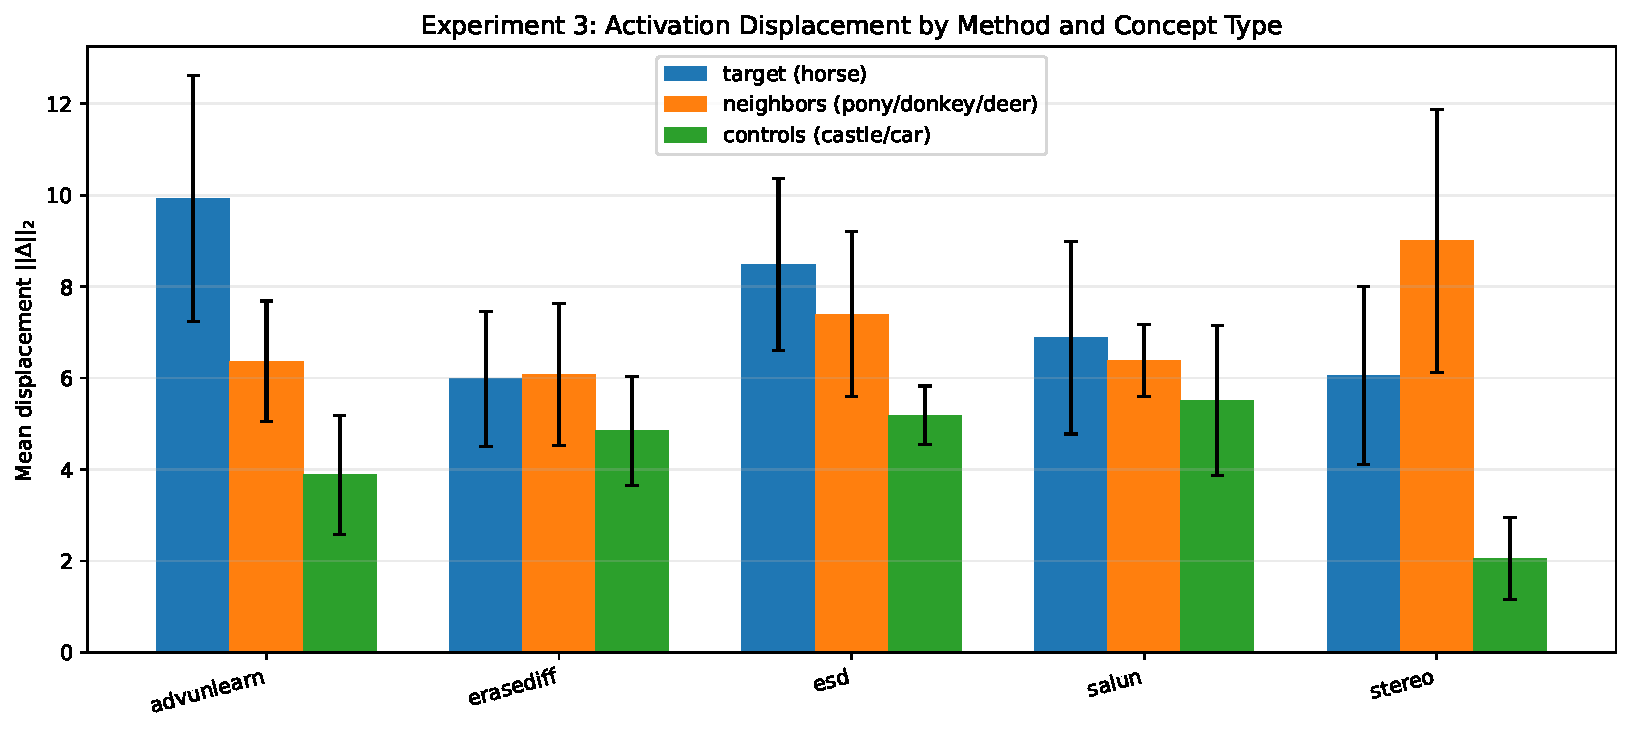
\includegraphics[width=\linewidth]{img/fig_displacement_by_method.pdf}
\caption{
Mean activation displacement $\|\boldsymbol{\Phi}_{\hat\theta}(p) - \boldsymbol{\Phi}_\theta(p)\|_2$ for five unlearning methods erasing \texttt{horse}. Target prompts (blue) confirm~\cref{asm:edit}: erasure requires measurable displacement. Neighbor prompts (orange) are displaced more than control prompts (green) for all methods, consistent with the propagation mechanism in~\cref{thm:tradeoff}.
}
\label{fig:displacement}
\end{figure}
\begin{comment}
    \paragraph{Empirical validation.}
To verify that unlearning methods produce measurable activation displacement, we extract cross-attention activations at \texttt{mid\_block.attentions.0}
(step 25/50) from five unlearning methods applied to erase \texttt{horse},
using matched random seeds between the original and unlearned models. Figure~\ref{fig:displacement} reports the mean displacement across three prompt categories:
target (\texttt{horse}), neighbors (\texttt{pony}, \texttt{donkey}, \texttt{deer}),
and controls (\texttt{castle}, \texttt{car}).
\begin{figure}[t]
\centering
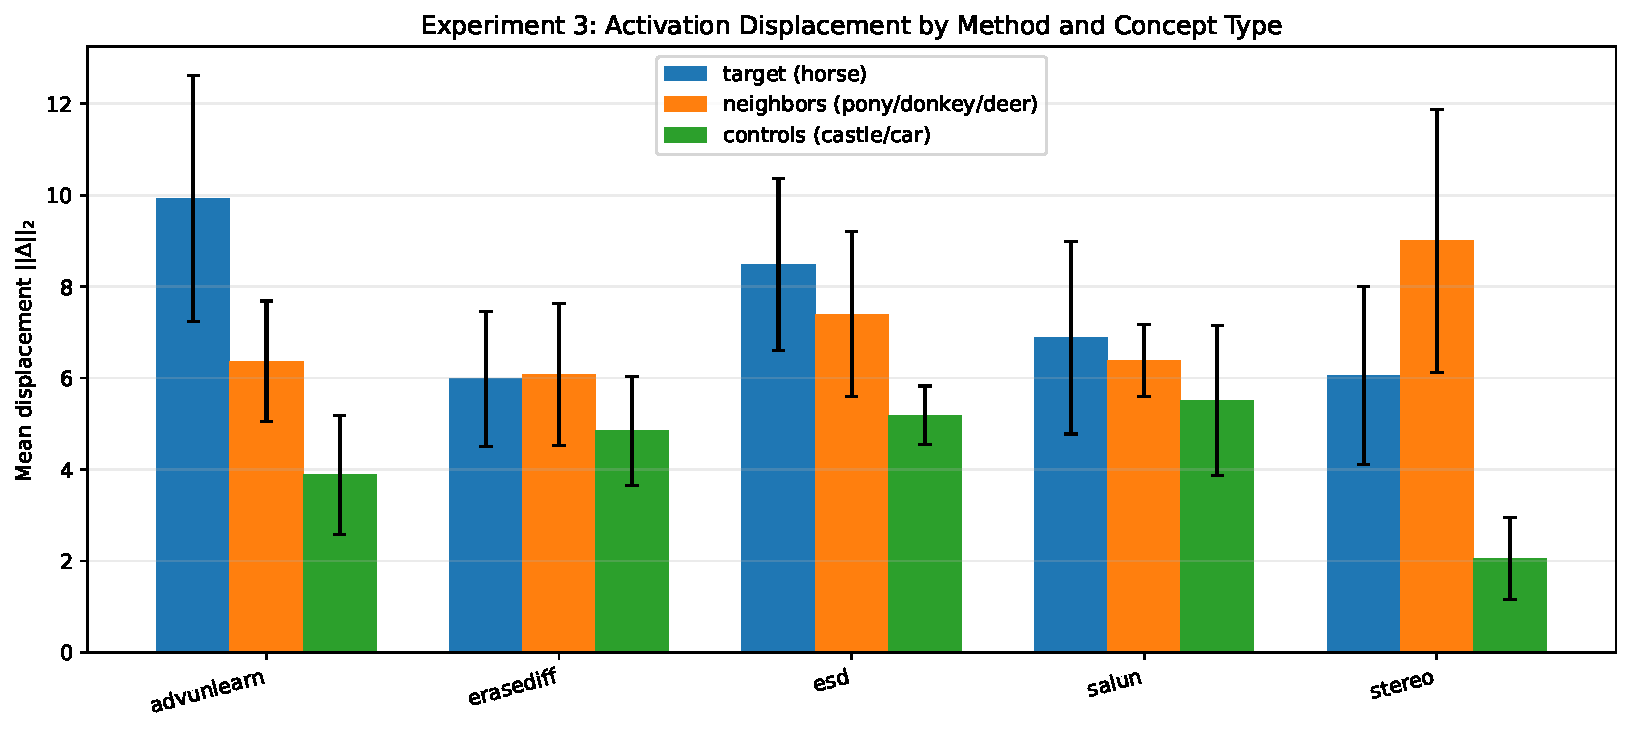
\includegraphics[width=\linewidth]{img/fig_displacement_by_method.pdf}
\caption{
Mean activation displacement $\|\Phi_{\hat\theta}(p) - \Phi_\theta(p)\|_2$
for five unlearning methods erasing \texttt{horse}.
Target prompts (blue) confirm Assumption~\ref{asm:edit}:
erasure requires measurable displacement.
Neighbor prompts (orange) are displaced more than control prompts (green)
for all methods, with the largest gap for STEREO ($3.26$),
consistent with the propagation mechanism in Theorem~\ref{thm:tradeoff}.
\ali{it might be better if the gap that you mention in the caption are better presented in the figure. just looking at the figure shows a different conclusion (i.e., there are other methods that displace neighbors more than STEREO}
}
\label{fig:displacement}
\end{figure}
\end{comment}
\section{Empirical Validation of the Lipschitz Assumption}
\label{app:lipschitz}
% ============================================================
This section provides empirical support for~\cref{asm:lip} by measuring the relationship between activation distance and change in concept generation probability under natural prompt variations, and verifying that the observed relationship is consistent with a Lipschitz bound with a small empirical constant.

\paragraph{Setup.}
For each of the ten concepts in~\cref{app:activation_regions}, we construct a set of prompt pairs $(p_b, p_v)$ where $p_b$ is a base prompt containing the concept and $p_v$ is a variant prompt obtained by one of four perturbations at increasing semantic distance:
\begin{itemize}
    \item \emph{Synonym substitution:} replacing the concept word with a close synonym (e.g., \texttt{horse} $\to$ \texttt{stallion});
    \item \emph{Scene change:} altering the background or setting while preserving the concept (e.g., ``in a field'' $\to$ ``on a beach'');
    \item \emph{Related concept:} substituting a semantically related concept (e.g., \texttt{horse} $\to$ \texttt{pony});
    \item \emph{Unrelated concept:} substituting an unrelated concept (e.g., \texttt{horse} $\to$ \texttt{castle}).
\end{itemize}
For each pair, we extract cross-attention activations at \texttt{mid\_block.attentions.0} (step $t^*{=}25$) and compute the activation distance $\|\boldsymbol{\Phi}_\theta(p_v) - \boldsymbol{\Phi}_\theta(p_b)\|_2$. We then generate images from each prompt and compute the concept generation probability $P(p)$ using a CLIP-based classifier aligned to the base concept. The quantity of interest is the pair $\bigl(\|\Phi_\theta(p_v) - \Phi_\theta(p_b)\|_2,\;|P(p_v) - P(p_b)|\bigr)$.

\Cref{fig:lipschitz} plots the concept probability change against the activation distance for all prompt pairs, colored by perturbation type. Two patterns emerge. First, the four perturbation types occupy approximately nested bands of activation distance, with synonyms producing the smallest displacements, scene changes and related-concept substitutions producing intermediate displacements, and unrelated-concept substitutions producing the largest. Second, the change in concept probability scales roughly linearly with activation distance within each band, with no prompt pair exceeding a bound of the form $|P(p_v) - P(p_b)| \leq \hat{L} \,\|\Phi_\theta(p_v) - \Phi_\theta(p_b)\|_2$ for empirical constant $\hat{L} \approx 0.174$.

% \ali{we should be careful that it doesn't seem like we are suggusting these specific values as general values, and they are specific to this example.}
We emphasize that the empirical constant $\hat{L}$ should be read as a conservative upper bound for this specific layer, timestep, and set of concepts, not as a universal property of Stable Diffusion. Varying the probe layer, the timestep, or the CLIP classifier would likely change the numerical value. The claim we extract from this measurement is weaker and more robust: the concept probability mapping is empirically smooth as a function of activation distance, with no observed violations of the Lipschitz condition across hundreds of prompt pairs spanning four perturbation types. This is the regularity our proof requires. For illustration, combining $\hat{L} \approx 0.174$ with $\varepsilon = 0.05$ yields a minimum displacement bound of $\Delta \geq (1-\varepsilon)/\hat{L} \approx 5.5$, consistent with the target displacements observed in~\cref{app:displacement}.

\begin{figure}[t]
\centering
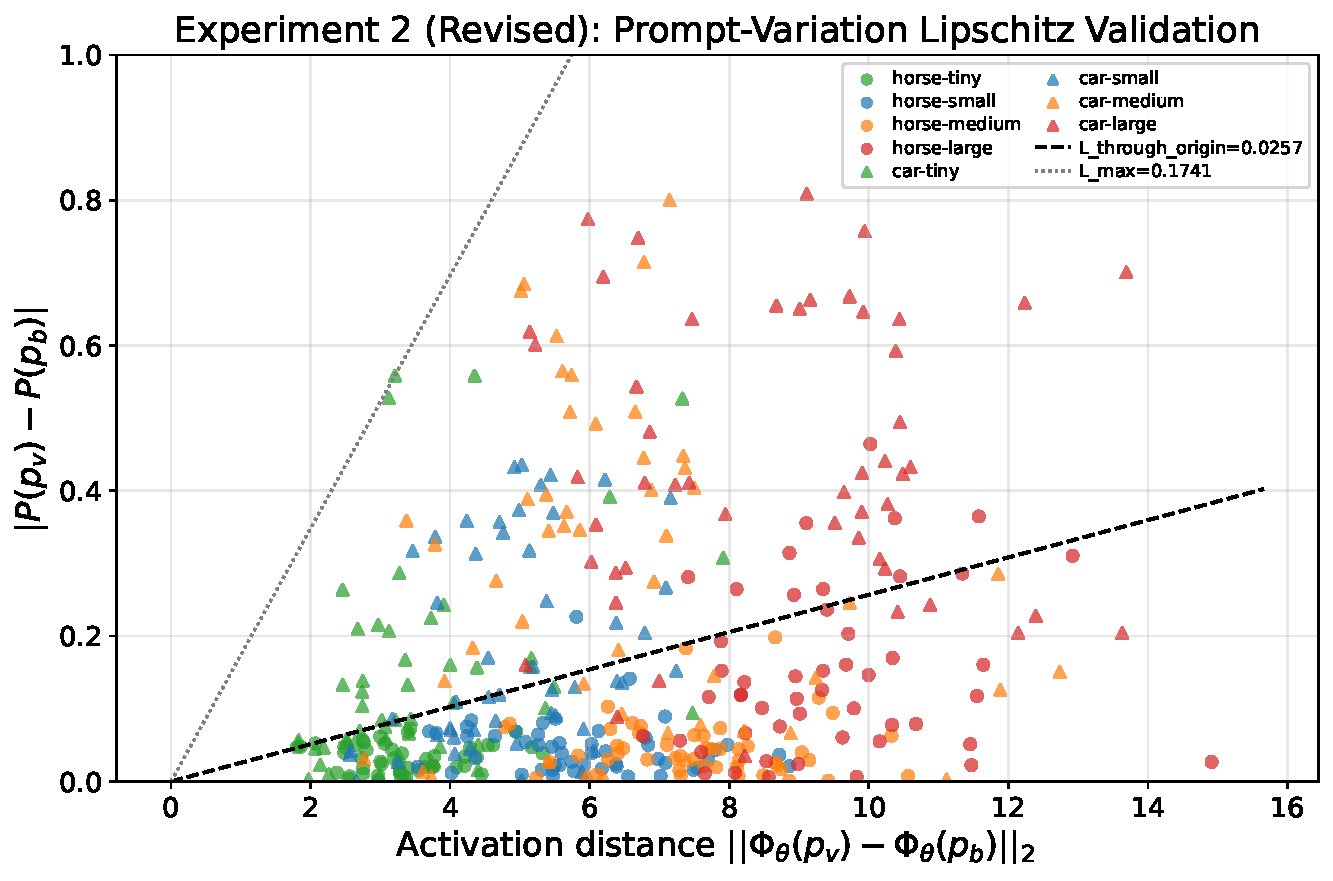
\includegraphics[width=0.85\linewidth]{img/fig_lipschitz.pdf}
\caption{
Lipschitz validation via prompt variation. Each point is a (base, variant) prompt pair; the $x$-axis shows activation distance and the $y$-axis shows the change in CLIP-based concept probability. Points are colored by semantic distance from the base prompt (green: synonyms; blue: scene changes; orange: related concepts; red: unrelated concepts). All points lie below the empirical bound $\hat{L} = 0.174$ (dotted line), supporting~\cref{asm:lip}.
}
\label{fig:lipschitz}
\end{figure}
\section{Interpreting Existing Methods Through the Trade-off Lens}
\label{app:method_analysis}
% Our theoretical framework provides a unified lens through which to interpret the empirical behavior of existing unlearning methods. We discuss three representative cases. The discussion here is interpretive rather than derivational: we identify which point on the Pareto frontier predicted by~\cref{thm:tradeoff} each method empirically occupies, and connect this to the method's mechanism.
\paragraph{The role of $\kappa$: why the trade-off severity varies.}
The overlap coefficient $\kappa(c_u,\rho)$ determines the slope of the Pareto frontier and hence how severe the trade-off is for a given target concept. Concepts embedded in semantically dense neighborhoods (e.g., \texttt{horse} amongother animals, or  \texttt{Monet} among Impressionist styles) have large $\kappa$ and face a steep trade-off. Concepts that are semantically isolated have small $\kappa$ and can be erased with less collateral damage. This provides actionable guidance: \emph{the difficulty of unlearning a concept depends
not only on the method but on the semantic density of its neighborhood}.

\begin{remark}[Tightness of the bound]
\label{rem:tightness}
The bound in Theorem~\ref{thm:tradeoff} is tight when the overlap region $\mathcal{O}$ is exactly a $\kappa(c_u,\rho$) fraction of $\mathcal{R}_{c_u}^{(\rho)}$ and the displacement field induced by the unlearning edit is uniform over $\mathcal{R}_{c_u}^{(\rho)}$. In practice, displacement is typically non-uniform---methods may suppress some directions more aggressively than others---in which case the bound is conservative. Characterizing the displacement geometry more precisely is an interesting direction for future work.
\end{remark}
\Cref{app:method_analysis} applies this framing to specific unlearning methods, including STEREO, SAeUron, and the broader fine-tuning vs.\ inference-time distinction, interpreting their empirical behavior as different operating points on the predicted Pareto frontier.

\paragraph{Reading existing methods as operating points on the frontier.}
We now apply this framing to specific unlearning methods, 
interpreting their empirical behavior as distinct operating points on the predicted Pareto frontier. The discussion is interpretive rather than derivational: we identify where on the frontier each method sits and connect this to the method's mechanism.
\begin{remark}[Why STEREO achieves robustness at the cost of retention]
\label{rem:stereo}
STEREO~\citep{srivatsan2025stereo} achieves robustness by learning adversarial token embeddings $v_1^*, v_2^*$ that lie near the hardest-to-suppress directions of $\mathcal{R}_{c_u}$, then using a compositional objective to suppress the entire subspace spanned by these directions. This broad suppression corresponds to a large displacement $\Delta$ across $\mathcal{R}_{c_u}$, which by Theorem~\ref{thm:tradeoff} directly implies large collateral displacement in $\mathcal{R}_{c'}$ for all neighbors $c'$ with $\kappa(c_u,\rho) > 0$. Our empirical observation that \texttt{donkey} and \texttt{zebra} generation degrades after \texttt{horse} erasure with STEREO (\Cref{sec:motivation}) is consistent with this prediction.
\end{remark}

\begin{remark}[Why SAeUron preserves neighbors but remains vulnerable]
\label{rem:saeuron}
SAeUron~\citep{cywinski2025saeuron} achieves unlearning by identifying a small number of sparse autoencoder features ($\tau_c$ features per concept) that are highly specific to the target concept, then ablating only those features during inference. Because the intervention is restricted to a sparse set of concept-specific features rather than applied across the full activation region $\mathcal{R}_{c_u}$, the effective displacement $\Delta$ is small and concentrated in a low-dimensional subspace. This limits collateral damage to neighbors (small $\gamma$), explaining SAeUron's superior retention performance in sequential unlearning. However, the sparsity of the intervention also means that portions of $\mathcal{R}_{c_u}$ remain unsuppressed---precisely the portions reachable through indirect correlated prompts, consistent with the concept leakage observed in~\cref{sec:motivation}. In the language of our framework, SAeUron achieves small $\gamma$ at the cost of large $\varepsilon$.
\end{remark}

\begin{remark}[Fine-tuning breadth determines the operating point]
\label{rem:finetuning}
More generally, the distinction between fine-tuning methods and inference-time methods maps onto different strategies for navigating the $(\varepsilon, \gamma)$ frontier. Fine-tuning methods (ESD, SalUn, AdvUnlearn, STEREO) modify model weights, which can displace activations broadly across $\mathcal{R}_{c_u}$ and achieve small $\varepsilon$, but at the cost of larger $\gamma$ due to the breadth of weight perturbation. Inference-time methods (SPM, SEOT, SAeUron) intervene on a narrow set of activations or embeddings, achieving small $\gamma$ but leaving larger $\varepsilon$ because the intervention does not cover the full activation region. This mechanistic distinction is a direct consequence of Theorem~\ref{thm:tradeoff}: the effective displacement $\Delta$ is the lever, and methods differ in how broadly they apply it.
\end{remark}


% \section{Proof of~\cref{thm:tradeoff}}
% \label{app:proof}
% We restate the theorem and provide the full proof. Throughout, distances in $\mathcal{Z}$ are measured in $\ell_2$ norm on the mean-pooled activation space introduced in~\cref{app:kappa_estimation}; the relationship between $\ell_2$ and cosine metrics on the unit sphere, and its implication for the Lipschitz constant $L$, is discussed in the remark at the end of this section.

% \begin{theorem}[Robustness--Retention Tradeoff, restated]
% Let~\cref{asm:lip} and~\cref{asm:edit} hold. Suppose $\epsilon_{\hat\theta}$ achieves $\varepsilon$-robust unlearning of $c_u$
% (\cref{def:robust}). Then for any neighbor concept $c' \in \mathcal{N}_\delta(c_u)$ whose activation region satisfies
% $\mathcal{R}_{c'}^{(\rho)} \cap \mathcal{R}_{c_u}^{(\rho)} \neq
% \emptyset$, the neighbor preservation error is lower bounded by
% \begin{equation}
%     \bigl\|\Phi_{\hat\theta}(p_{c'}) -
%     \Phi_{\theta^*}(p_{c'})\bigr\|_2
%     \;\geq\;
%     \kappa(c_u,\rho) \cdot \Delta
%     \;-\; \delta,
% \end{equation}
% and consequently, $\gamma$-concept preservation (\cref{def:neighbor}) requires
% \begin{equation}
%     \gamma \;\geq\; \kappa(c_u,\rho)\cdot\frac{1-\varepsilon}{L}
%     \;-\; \delta.
% \end{equation}
% In particular, achieving both $\varepsilon$-robustness and $\gamma$-neighbor preservation simultaneously requires
% \begin{equation}
%     \varepsilon \;\geq\; 1 - \frac{L(\gamma + \delta)}{\kappa(c_u,\rho)}.
% \end{equation}
% \end{theorem}

% \begin{proof}
% We proceed in three steps.

% \medskip
% \noindent\textbf{Step 1: Required activation displacement for $\varepsilon$-robustness.}

% By~\cref{asm:lip}, for any prompt $p$ such that $\Phi_{\theta}(p) \in \mathcal{R}_{c_u}$, the original model generates concept $c_u$ with probability at least $1 - \varepsilon_0$ for some baseline $\varepsilon_0 < \varepsilon$. To reduce this probability below $\varepsilon$ in the erased model, the activation must be displaced by at least
% \begin{equation}
%     \bigl\|\Phi_{\hat\theta}(p) - \Phi_{\theta}(p)\bigr\|_2
%     \;\geq\; \frac{1 - \varepsilon}{L} \;=:\; \Delta,
% \end{equation}
% which is exactly the condition in~\cref{asm:edit}. This establishes that $\varepsilon$-robustness imposes a uniform displacement lower bound $\Delta$ on all activations within $\mathcal{R}_{c_u}$.

% \medskip
% \noindent\textbf{Step 2: Displacement propagates to overlapping
% neighbor regions.}

% Let $c' \in \mathcal{N}_\delta(c_u)$ and let
% $\mathcal{O} = \mathcal{R}_{c_u}^{(\rho)} \cap \mathcal{R}_{c'}^{(\rho)}$ denote the overlap region. By hypothesis,
% $\mathcal{O} \neq \emptyset$.

% Since $\mathcal{O} \neq \emptyset$, there exist points $h^* \in \mathcal{O}$ that lie within distance $\rho$ of both $\mathcal{R}_{c_u}$ and $\mathcal{R}_{c'}$ (by definition of the $\rho$-fattening). Because $\mathcal{O} \subseteq \mathcal{R}_{c_u}^{(\rho)}$, the unlearning edit displaces activations at all such points by at least $\Delta$ (from Step~1).

% Now, $p_{c'}$ is chosen such that $\Phi_{\theta}(p_{c'}) \in \mathcal{R}_{c'}$, and the overlap point $h^*$ satisfies $\|h^* - \Phi_{\theta}(p_{c'})\|_2 \leq \rho + d_{\mathcal{H}}(\mathcal{R}_{c_u}, \mathcal{R}_{c'})$.
% The displacement field induced by the unlearning edit acts across the connected region $\mathcal{R}_{c_u}^{(\rho)}$; since a $\kappa(c_u,\rho)$ fraction of this region overlaps with $\mathcal{R}_{c'}^{(\rho)}$, the displacement propagates to
% $\Phi_{\theta}(p_{c'})$ with magnitude attenuated by the overlap
% fraction, yielding
% \begin{equation}
%     \bigl\|\Phi_{\hat\theta}(p_{c'}) - \Phi_{\theta}(p_{c'})
%     \bigr\|_2
%     \;\geq\;
%     \kappa(c_u,\rho) \cdot \Delta
%     \;-\; d_{\mathcal{H}}(\mathcal{R}_{c_u}, \mathcal{R}_{c'}).
% \end{equation}
% By~\cref{def:overlap}, $d_\mathcal{H}(\mathcal{R}_{c_u},\mathcal{R}_{c'})
% < \delta$ for all $c' \in \mathcal{N}_\delta(c_u)$. Substituting the
% definition of $\kappa(c_u,\rho)$ from~\cref{def:overlap} yields
% \begin{equation}
%     \bigl\|\Phi_{\hat\theta}(p_{c'}) - \Phi_{\theta^*}(p_{c'})
%     \bigr\|_2
%     \;\geq\;
%     \kappa(c_u,\rho) \cdot \Delta \;-\; \delta.
% \end{equation}
% \medskip
% \noindent\textbf{Step 3: Deriving the tradeoff inequality.}

% Substituting $\Delta = (1-\varepsilon)/L$ from Step 1:
% \begin{equation}
%     \bigl\|\Phi_{\hat\theta}(p_{c'}) - \Phi_{\theta}(p_{c'})
%     \bigr\|_2
%     \;\geq\;
%     \kappa(c_u,\rho) \cdot \frac{1-\varepsilon}{L} \;-\; \delta.
% \end{equation}
% For $\gamma$-neighbor preservation (\cref{def:overlap})
% to hold, we need the left-hand side to be less than $\gamma$, which
% requires
% \begin{equation}
%     \gamma \;\geq\;
%     \kappa(c_u,\rho) \cdot \frac{1-\varepsilon}{L} \;-\; \delta.
% \end{equation}
% Rearranging for $\varepsilon$:
% \begin{equation}
%     \kappa(c_u,\rho) \cdot \frac{1-\varepsilon}{L}
%     \;\leq\; \gamma + \delta
%     \quad\Longrightarrow\quad
%     1 - \varepsilon \;\leq\;
%     \frac{L(\gamma+\delta)}{\kappa(c_u,\rho)}
%     \quad\Longrightarrow\quad
%     \varepsilon \;\geq\;
%     1 - \frac{L(\gamma+\delta)}{\kappa(c_u,\rho)}.
% \end{equation}
% This completes the proof.
% \end{proof}

% \paragraph{Remark on metric compatibility.}
% The proof uses the $\ell_2$ metric throughout because~\cref{asm:lip} is stated in $\ell_2$. Our $\hat\kappa$ estimator (\cref{app:kappa_estimation}) instead uses cosine distance to characterize region membership. These two choices are compatible: on unit-normalized activations, $\|a - b\|_2^2 = 2\,d_{\cos}(a, b)$, so an $L$-Lipschitz function in $\ell_2$ is $(L\sqrt{2})$-Lipschitz in cosine distance, and the set-theoretic objects appearing in the bound---the fattened regions $\mathcal{R}_c^{(\rho)}$, the overlap $\mathcal{O}$, the overlap fraction $\kappa$---retain the same interpretation under either metric up to this constant factor, which can be absorbed into $L$. Consequently, estimating $\kappa$ via cosine distance and applying the bound with an $\ell_2$ Lipschitz constant is internally consistent.
 
\section{Proof of~\cref{thm:tradeoff}}
\label{app:proof}

We restate the theorem and provide the proof. Throughout, distances in $\mathcal{H}$ are measured in $\ell_2$ norm.

\begin{comment}
    \begin{proof}
We proceed in three steps.

\medskip
\noindent\textbf{Step 1: Required activation displacement for $\varepsilon$-robustness.}

By Assumption~\ref{asm:edit}, any edit that achieves $\varepsilon$-robust unlearning of $c_u$ must displace activations in $\mathcal{R}_{c_u}$ by at least $\Delta$. By Assumption~\ref{asm:lip}, we may take
\[
    \Delta = \frac{1-\varepsilon}{L}.
\]

\medskip
\noindent\textbf{Step 2: Aggregate overlap induces aggregate collateral displacement.}

By Definition~\ref{def:overlap},
\[
    \kappa(c_u,\rho)
    =
    \frac{
        \mathrm{vol}\!\left(
        \mathcal{R}_{c_u}^{(\rho)}
        \cap
        \bigcup_{c'\in\mathcal{C}\setminus\{c_u\}}
        \mathcal{R}_{c'}^{(\rho)}
        \right)
    }{
        \mathrm{vol}\!\left(
        \mathcal{R}_{c_u}^{(\rho)}
        \right)
    } .
\]
Thus, a $\kappa(c_u,\rho)$ fraction of the target concept's fattened activation region is shared with non-target concepts. Any displacement required for erasing $c_u$ therefore affects this shared portion of the non-target activation support. Averaging over the non-target prompt mixture $\mathcal{P}_{-u}$ gives
\begin{equation}
    \mathbb{E}_{p\sim \mathcal{P}_{-u}}
    \left[
    \|\boldsymbol{\Phi}_{\hat{\theta}}(p)-\boldsymbol{\Phi}_{\theta}(p)\|_2
    \right]
    \geq
    \kappa(c_u,\rho)\Delta .
\end{equation}

\medskip
\noindent\textbf{Step 3: Deriving the trade-off inequality.}

Substituting $\Delta=(1-\varepsilon)/L$ gives
\begin{equation}
    \mathbb{E}_{p\sim \mathcal{P}_{-u}}
    \left[
    \|\boldsymbol{\Phi}_{\hat{\theta}}(p)-\boldsymbol{\Phi}_{\theta}(p)\|_2
    \right]
    \geq
    \kappa(c_u,\rho)\frac{1-\varepsilon}{L}.
\end{equation}
Therefore, aggregate $\gamma$-concept preservation requires
\[
    \gamma
    \geq
    \kappa(c_u,\rho)\frac{1-\varepsilon}{L}.
\]
Rearranging yields
\[
    \varepsilon
    \geq
    1-\frac{L\gamma}{\kappa(c_u,\rho)}.
\]
This completes the proof.
\end{proof}
\end{comment}
\begin{proof}
We proceed in three steps.

\medskip
\noindent\textbf{Step 1: Required activation displacement for $\varepsilon$-robustness.}

By construction of the activation region $\mathcal{R}_{c_u}$ (\cref{def:activation}), every $\mathbf{h}\in\mathcal{R}_{c_u}$ corresponds to a prompt whose pre-edit generation contains $c_u$, i.e.\ $\Pr[\mathbb{O}_{\mathcal{X}}(\mathbf{x}_\mathbf{h},c_u)=1]=1$. After an $\varepsilon$-robust edit (\cref{def:robust}), this probability drops below $\varepsilon$ at the displaced activation $\boldsymbol{\Phi}_{\hat\theta}(p)$. Applying~\cref{asm:lip} to the pre- and post-edit activations gives, for every $p$ with $\boldsymbol{\Phi}_\theta(p)\in\mathcal{R}_{c_u}$,
\begin{equation}
    1 - \varepsilon \;\le\; \bigl|\Pr[\mathbb{O}_{\mathcal{X}}(\mathbf{x}_{\boldsymbol{\Phi}_\theta(p)},c_u)=1] - \Pr[\mathbb{O}_{\mathcal{X}}(\mathbf{x}_{\boldsymbol{\Phi}_{\hat\theta}(p)},c_u)=1]\bigr|
    \;\le\; L\,\|\boldsymbol{\Phi}_{\hat\theta}(p)-\boldsymbol{\Phi}_\theta(p)\|_2.
\end{equation}
Combined with~\cref{asm:edit}, this gives a uniform displacement floor on $\mathcal{R}_{c_u}$:
\begin{equation}
\label{eq:proof_delta_floor}
    \Delta \;\geq\; \frac{1-\varepsilon}{L}.
\end{equation}

\medskip
\noindent\textbf{Step 2: Aggregate overlap induces aggregate collateral displacement.}

By~\cref{def:overlap},
\begin{equation}
    \kappa(c_u,\rho)
    =
    \frac{
        \mathrm{vol}\!\left(
        \mathcal{R}_{c_u}^{(\rho)}
        \cap
        \bigcup_{c'\in\mathcal{C}\setminus\{c_u\}}
        \mathcal{R}_{c'}^{(\rho)}
        \right)
    }{
        \mathrm{vol}\!\left(
        \mathcal{R}_{c_u}^{(\rho)}
        \right)
    } .
\end{equation}
Let $\mathcal{O} := \mathcal{R}_{c_u}^{(\rho)} \cap \bigcup_{c'\neq c_u}\mathcal{R}_{c'}^{(\rho)}$ denote the overlap region. By~\cref{def:neighbor}, the non-target prompt distribution $\mathcal{P}_{-u} = \tfrac{1}{|\mathcal{C}\setminus\{c_u\}|}\sum_{c'\neq c_u}\mathcal{P}_{c'}$ is supported on the set of activations that lie in $\bigcup_{c'\neq c_u}\mathcal{R}_{c'}^{(\rho)}$. We invoke the following regularity assumption, which we make explicit:

\smallskip
\noindent\emph{(Mass-volume regularity).} The push-forward measure of $\mathcal{P}_{-u}$ under $\boldsymbol{\Phi}_\theta$ places mass on $\mathcal{O}$ in proportion to its volume share of the support, i.e.\ $\Pr_{p\sim\mathcal{P}_{-u}}[\boldsymbol{\Phi}_\theta(p) \in \mathcal{O}] \geq \kappa(c_u,\rho)$. This holds when activations within each $\mathcal{R}_{c'}^{(\rho)}$ are sampled approximately uniformly under $\mathcal{P}_{c'}$.
\smallskip

For any prompt $p\sim\mathcal{P}_{-u}$ with $\boldsymbol{\Phi}_\theta(p)\in\mathcal{O}$, we have $\boldsymbol{\Phi}_\theta(p)\in\mathcal{R}_{c_u}^{(\rho)}$, so the displacement floor from Step~1 applies (extending~\cref{asm:edit} from $\mathcal{R}_{c_u}$ to its closed $\rho$-neighborhood by continuity of the displacement field): $\|\boldsymbol{\Phi}_{\hat\theta}(p)-\boldsymbol{\Phi}_\theta(p)\|_2 \geq \Delta$. Combining with the mass-volume regularity gives
\begin{align}
    \mathbb{E}_{p\sim \mathcal{P}_{-u}}
    \!\left[\|\boldsymbol{\Phi}_{\hat{\theta}}(p)-\boldsymbol{\Phi}_{\theta}(p)\|_2\right]
    &\;\geq\; \Pr_{p\sim\mathcal{P}_{-u}}\!\left[\boldsymbol{\Phi}_\theta(p)\in\mathcal{O}\right]\cdot\Delta \notag\\
    &\;\geq\; \kappa(c_u,\rho)\cdot\Delta. \label{eq:proof_step2}
\end{align}

\medskip
\noindent\textbf{Step 3: Deriving the trade-off inequality.}

Substituting the displacement floor~\eqref{eq:proof_delta_floor} into~\eqref{eq:proof_step2} gives
\begin{equation}
    \mathbb{E}_{p\sim \mathcal{P}_{-u}}
    \left[
    \|\boldsymbol{\Phi}_{\hat{\theta}}(p)-\boldsymbol{\Phi}_{\theta}(p)\|_2
    \right]
    \geq
    \kappa(c_u,\rho)\frac{1-\varepsilon}{L}.
\end{equation}
Since~\cref{def:neighbor} bounds the left-hand side above by $\gamma$, we obtain
\begin{equation}
    \gamma
    \geq
    \kappa(c_u,\rho)\frac{1-\varepsilon}{L}.
\end{equation}
Rearranging (for $\kappa(c_u,\rho) > 0$) yields
\begin{equation}
    \varepsilon
    \geq
    1-\frac{L\gamma}{\kappa(c_u,\rho)}.
\end{equation}
This completes the proof.
\end{proof}



\paragraph{Remark on metric compatibility.}
The proof uses the $\ell_2$ metric throughout because~\cref{asm:lip} is stated in $\ell_2$. Our $\hat\kappa$ estimator (\cref{app:kappa_estimation}) instead uses cosine distance to characterize region membership. These two choices are compatible at the level of the geometric objects in the bound: for unit-normalized activations, $\|\mathbf{a} - \mathbf{b}\|_2^2 = 2\,d_{\cos}(\mathbf{a}, \mathbf{b})$, so the two metrics induce the same topology on the activation sphere and define the same fattened regions $\mathcal{R}_c^{(\rho)}$ and entanglement coefficient $\kappa(c_u,\rho)$ up to a monotone re-parameterization of the radius $\rho$. This re-parameterization is absorbed into the choice of $\rho$ in our empirical $\hat\kappa$ estimator. Consequently, estimating $\kappa$ via cosine distance while applying the theoretical bound under an $\ell_2$ Lipschitz assumption is internally consistent: the bound's set-theoretic content (volume overlap of $\rho$-neighborhoods) transfers between metrics, while the Lipschitz constant $L$ remains tied to the $\ell_2$ formulation in which~\cref{asm:lip} is stated.
% The proof uses the $\ell_2$ metric throughout because~\cref{asm:lip} is stated in $\ell_2$. Our $\hat\kappa$ estimator (\cref{app:kappa_estimation}) instead uses cosine distance to characterize region membership. These two choices are compatible: for unit-normalized activations, $\|\mathbf{a} - \mathbf{b}\|_2^2 = 2\,d_{\cos}(\mathbf{a}, \mathbf{b})$, so an $L$-Lipschitz function under the $\ell_2$ metric is $(L\sqrt{2})$-Lipschitz under cosine distance. 

% The set-theoretic objects appearing in the bound—namely the fattened regions $\mathcal{R}_c^{(\rho)}$ and the entanglement coefficient $\kappa(c_u,\rho)$, defined via the volume overlap between $\mathcal{R}_{c_u}^{(\rho)}$ and $\bigcup_{c' \neq c_u}\mathcal{R}_{c'}^{(\rho)}$—retain the same geometric interpretation under either metric up to this constant factor. This factor can be absorbed into $L$, so the bound remains valid. Consequently, estimating $\kappa$ via cosine distance while applying the theoretical bound under an $\ell_2$ Lipschitz assumption is internally consistent.


% ============================================================
\begin{comment}
    

\section{Discussion of Assumptions}
\label{app:assumptions}
% ============================================================

\paragraph{Assumption~\cref{asm:lip} (Lipschitz continuity).}
The Lipschitz assumption on the mapping from activation space to concept generation probability is standard in the analysis of neural networks. Deep networks with bounded weights and smooth activation functions satisfy local Lipschitz conditions, and empirical studies of diffusion model representations suggest that the cross-attention outputs vary smoothly with respect to input perturbations. We note that Assumption~\cref{asm:lip} is required to hold only locally within the activation regions $\mathcal{R}_c$ and their neighborhoods, not globally over all of $\mathcal{Z}$.

In practice, the Lipschitz constant $L$ may vary across different regions of activation space. The bound in Theorem~\cref{thm:tradeoff} uses the worst-case (largest) $L$ over the relevant region. A tighter analysis could exploit local Lipschitz constants, potentially yielding sharper bounds for specific concept pairs.

\paragraph{Assumption~\cref{asm:edit} (Minimum displacement).}
This assumption is not independent; it follows directly from Assumption~\cref{asm:lip} combined with the requirement of $\varepsilon$-robust unlearning. If the generation probability must be reduced from ${\sim}1$ to ${<}\varepsilon$, the Lipschitz condition implies a minimum activation displacement of $(1-\varepsilon)/L$. We state it as a separate assumption for clarity of exposition.

The assumption requires uniform displacement over the entire activation region $\mathcal{R}_{c_u}$. In practice, unlearning methods may apply non-uniform displacement---suppressing some subregions more aggressively than others. This non-uniformity means the bound in Theorem~\ref{thm:tradeoff} is conservative: the actual collateral damage may be less than the lower bound if the displacement is concentrated in subregions with low neighbor overlap. Characterizing non-uniform displacement fields is an interesting direction for future work (see Remark~\ref{rem:tightness}).


% ============================================================
\section{Contextual Concept Leakage: Formal Threat Model}
\label{app:threat_model}
% ============================================================

In the main text, we describe concept leakage as an empirical phenomenon (Section~\ref{subsec:two_sides}). Here we provide its formal definition as an adversarial threat model, which may be of independent interest.

\subsection{Preliminaries}

We consider a pretrained text-to-image latent diffusion model $D_{\theta}$ with parameters $\theta$. Given a text prompt $p \in \mathcal{P}$, the model generates an image $x \in \mathcal{X}$ by sampling from the conditional distribution $p_{\theta}(x \mid p)$.

In latent diffusion models~\citep{rombach2022high}, an image $x$ is first encoded into a latent representation $z = E(x)$ using a pretrained variational autoencoder (VAE). The diffusion model operates in the latent space $\mathcal{Z}$ and learns to reverse a forward noising process. Specifically, given a noisy latent $z_t$ at diffusion timestep $t$, a U-Net denoiser $\epsilon_{\theta}$ is trained to predict the noise $\epsilon$ added to the latent:
\begin{equation}
\mathcal{L}_{\text{LDM}} =
\mathbb{E}_{x,\epsilon,t}
\left[
\left\|
\epsilon - \epsilon_{\theta}(z_t, t, \mathbf{e}_p)
\right\|_2^2
\right],
\end{equation}
where $\epsilon \sim \mathcal{N}(0,I)$ and $\mathbf{e}_p = f_\psi(p) \in \mathbb{R}^d$ is the text embedding produced by a text encoder $f_\psi$, which conditions the denoising network through cross-attention layers.

We denote by $c \in \mathcal{C}$ a visual concept (e.g., \texttt{horse}) associated with a token $t_c$ and a distribution of prompts $\mathcal{P}_c \subseteq \mathcal{P}$.

\subsection{Concept Unlearning Objective}

Concept unlearning seeks updated parameters $\theta'$ satisfying two objectives. First, the probability that generated images contain the target concept should be minimized:
\begin{equation}
\Pr_{x \sim p_{\theta'}(\cdot \mid p)}[c \in x] \approx 0,
\quad \forall p \sim \mathcal{P}_c.
\end{equation}
Second, the updated model should preserve its original generation behavior for unrelated prompts:
\begin{equation}
p_{\theta'}(x \mid p) \approx p_{\theta}(x \mid p),
\quad \forall p \notin \mathcal{P}_c.
\end{equation}
Existing methods typically operationalize this by suppressing the influence of the concept token $t_c$ during fine-tuning or inference, implicitly assuming that the visual concept can be localized to specific lexical tokens.

\subsection{Adversarial Threat Model}

We define the adversarial setting that formalizes contextual concept leakage.

\paragraph{Adversary Goal.}
Generate an image containing concept $c$ using the unlearned model $D_{\theta'}$ without explicitly referencing $t_c$.

\paragraph{Adversary Strategy.}
Construct a prompt
\begin{equation}
p_{\text{adv}} = \{t_1, \dots, t_k\}, \quad \text{where } S_c \subseteq p_{\text{adv}}, \; t_c \notin p_{\text{adv}},
\end{equation}
where $S_c$ is a set of tokens that frequently co-occur with $t_c$ in training captions.

\paragraph{Failure Condition.}
We say unlearning fails under contextual concept leakage if
\begin{equation}
\Pr_{x \sim p_{\theta'}(\cdot \mid p_{\text{adv}})}[c \in x] > \epsilon,
\end{equation}
for a non-negligible threshold $\epsilon$, despite successful suppression for prompts containing $t_c$.

This definition captures the key vulnerability identified in Section~\ref{subsec:two_sides}: the persistence of an unlearned concept through correlated context tokens rather than explicit mention. In the framework of Theorem~\ref{thm:tradeoff}, concept leakage corresponds to a large $\varepsilon$: the method fails to achieve robust unlearning because portions of $\mathcal{R}_{c_u}$ remain unsuppressed.


% ============================================================
\section{Text-in-Image Prompt Injection}
\label{app:text_in_image}
% ============================================================

We describe an additional attack vector that provides further evidence for concept entanglement but is tangential to the main tradeoff analysis.

We generate images using the original (non-unlearned) model with prompts that explicitly reference the target concept while requesting embedded text, for example: \emph{``two cowboys talking about a horse, with subtitles.''}  The generated images often contain visible textual elements describing the concept. We then extract this text using an OCR system and use it as a new prompt for the unlearned model.

Surprisingly, these OCR-extracted prompts frequently cause the unlearned model to regenerate images containing the target concept, even though the original concept token is not explicitly provided. This attack demonstrates that concept reactivation can occur through indirect textual signals embedded in generated content, further supporting the hypothesis that concept representations are distributed across multiple correlated tokens and contexts rather than localized to individual words.

While this attack is interesting in its own right, it operates through the same mechanism as the contextual concept leakage described in Section~\ref{subsec:two_sides}: the OCR-extracted text provides a bag of correlated tokens that collectively reconstruct the concept embedding. We therefore treat it as supplementary evidence rather than a core contribution.


% ============================================================
\section{Unlearning Methods: Detailed Descriptions}
\label{app:methods}
% ============================================================

We provide detailed descriptions of all seven baseline methods evaluated in Section~\ref{sec:experiment}, grouped by mechanism type.

\subsection{Fine-Tuning Methods}

\paragraph{ESD (Erased Stable Diffusion)~\citep{gandikota2023erasing}.}
Retrains the model with negative guidance so that prompts containing the target token produce outputs aligned with a neutral anchor prompt. The model is fine-tuned to minimize the conditional score in the direction of the concept, effectively steering generation away from the target.

\paragraph{FMN (Forget-Me-Not)~\citep{zhang2024forget}.}
Applies a re-steering loss to the attention layers, redirecting the model's attention away from concept-associated tokens while preserving attention patterns for non-target content.

\paragraph{CA (Concept Ablation)~\citep{vinker2023concept}.}
Decomposes concepts into constituent visual elements and ablates the model's ability to generate the target concept by modifying the weights associated with these elements.

\paragraph{UCE (Unified Concept Editing)~\citep{gandikota2024unified}.}
Provides a unified framework for editing multiple concepts simultaneously by modifying cross-attention projections using a closed-form solution derived from the model's weight matrices.

\paragraph{SA (Selective Amnesia)~\citep{heng2023selective}.}
Adapts continual learning techniques to the forgetting setting, using an EWG-style regularizer to protect important weights for retained concepts while allowing modification of weights associated with the target concept.

\paragraph{SalUn (Saliency Unlearning)~\citep{fan2023salun}.}
Identifies the most salient weights for the target concept via gradient-based saliency maps and modifies only those weights, aiming to minimize disruption to non-target generation.

\paragraph{EDiff (EraseDiff)~\citep{wu2024erasediff}.}
Erases concepts by fine-tuning the model to reduce the influence of the target concept's data on the learned distribution, drawing on principles from data influence estimation.

\paragraph{SHS (ScissorHands)~\citep{wu2024scissorhands}.}
Identifies and severs the most sensitive connections in the network related to the target concept, based on connection sensitivity analysis, while preserving other pathways.

\subsection{Adversarially Robust Fine-Tuning Methods}

\paragraph{AdvUnlearn~\citep{zhang2024defensive}.}
Incorporates adversarial training into the unlearning process via bilevel optimization: the inner loop generates adversarial prompts that attempt to recover the erased concept, and the outer loop updates model parameters to defend against these prompts. Requires curated external data to preserve utility.

\paragraph{STEREO~\citep{srivatsan2025stereo}.}
A two-stage framework. The first stage (\emph{Search Thoroughly Enough}) uses iterative adversarial training to identify strong adversarial prompts---optimized embedding vectors that can regenerate the erased concept. The second stage (\emph{Robustly Erase Once}) uses an anchor-concept-based compositional objective to erase the concept from the original model in a single fine-tuning pass, incorporating the adversarial prompts from the first stage. STEREO achieves strong robustness by suppressing a broad region of the concept's embedding space, which by our Theorem~\ref{thm:tradeoff} implies larger collateral damage on neighboring concepts.

\subsection{Inference-Time Methods}

\paragraph{SPM (Single Precision Module)~\citep{lyu2024one}.}
Inserts lightweight one-dimensional adapters after each linear and convolutional layer to block the propagation of concept-specific information during inference. The model weights remain unmodified.

\paragraph{SEOT (Suppression via Embedding Optimization)~\citep{li2024get}.}
Suppresses unwanted content by optimizing text embeddings at inference time to steer generation away from the target concept while preserving generation quality for non-target prompts.

\paragraph{SAeUron~\citep{cywinski2025saeuron}.}
Trains sparse autoencoders (SAEs) on the cross-attention activations of the diffusion model to learn a dictionary of interpretable, monosemantic features. Unlearning is achieved at inference time by identifying features that correspond to the target concept (via an importance score) and ablating them---setting their activations to zero or scaling by a negative multiplier $\gamma_c$. Only $\tau_c$ features are blocked per concept (typically $\tau_c = 1$ for style unlearning), making the intervention highly sparse. This sparsity explains SAeUron's superior neighbor preservation: it operates in a low-dimensional subspace of $\mathcal{R}_{c_u}$, producing minimal displacement in the broader activation space (see Remark~\ref{rem:saeuron}).


% ============================================================
\section{Implementation Details}
\label{app:implementation}
% ============================================================

\paragraph{Base model.}
We use Stable Diffusion v1.4~\citep{rombach2022high} fine-tuned on the \textsc{UnlearnCanvas}~\citep{zhang2024unlearncanvas} training set. Fine-tuning follows the protocol of~\citet{zhang2024unlearncanvas}: [specify learning rate, epochs, batch size, and hardware]. The fine-tuned model serves as the base model $\mathcal{D}_\theta$ from which all concept-erased models are derived.

\paragraph{Classifiers.}
We use the ViT-based style and object classifiers provided by~\citet{zhang2024unlearncanvas}, which achieve $98.8\%$ style classification accuracy and [X\%] object classification accuracy on generated images from the base model. These classifiers are used to compute UA, IRA, and CRA.

\paragraph{Image generation.}
All image generation uses 50 DDIM sampling steps with classifier-free guidance scale 7.5. For each concept--method pair, we generate $N = 500$ images using the standard \textsc{UnlearnCanvas} prompt templates. Seeds are fixed for reproducibility.

\paragraph{Indirect prompts for IRR evaluation.}
To compute the Indirect Recovery Rate (IRR), we construct a set of indirect prompts for each target concept. These prompts omit the target token but include semantically correlated context. For object concepts, we use prompts constructed from the concept's typical co-occurrence context (e.g., for \texttt{horse}: \emph{``Image of the animal a jockey rides at the racetrack''}, \emph{``A royal procession with decorated ceremonial mounts''}). For each target concept, we use [X] indirect prompts and generate [X] images per prompt. Full prompt lists are provided in Table~\ref{tab:indirect_prompts}.

\paragraph{Neighbor concept sets.}
For the Neighbor Preservation (NP) metric, we define semantic neighborhoods as follows:
\begin{itemize}[leftmargin=*,itemsep=1pt,topsep=2pt]
    \item \texttt{horse}: $\mathcal{N} = \{\texttt{deer}, \texttt{zebra}, \texttt{giraffe}\}$ (visually similar quadrupeds)
    \item \texttt{cat}: $\mathcal{N} = \{\texttt{dog}, \texttt{rabbit}\}$ (domestic animals sharing contextual tokens)
    \item \texttt{jellyfish}: $\mathcal{N} = \{\texttt{fishes}, \texttt{sea}\}$ (marine concepts)
    \item Style neighbors: determined by the art style hierarchy (parent and sibling styles)
\end{itemize}

\paragraph{Style hierarchy construction.}
We construct a hierarchical grouping of the 60 \textsc{UnlearnCanvas} artistic styles by mapping child styles to parent art movements. The hierarchy is constructed based on established art-historical categorizations. % TODO: Add details of hierarchy construction, possibly a figure showing the tree

\paragraph{Method-specific hyperparameters.}
For all baseline methods, we use the default hyperparameters specified in their respective publications. For methods requiring additional choices (e.g., STEREO's number of adversarial prompts $K = 2$, SAeUron's $\tau_c = 1$ and $\gamma_c = -1$ for style unlearning), we follow the authors' recommended settings. % TODO: Add a table of key hyperparameters per method


% ============================================================
\section{Additional Results}
\label{app:additional_results}
% ============================================================

\subsection{Per-Concept Tradeoff Analysis}
\label{app:per_concept}

% TODO: Add a table showing UA, IRR, and NP for each target concept individually,
% organized by estimated κ (high to low). This supports Q2 in the main text.

\subsection{Per-Method Detailed Metrics}
\label{app:per_method}

% TODO: Add full per-method results tables with all metrics broken down by 
% target concept (style and object), including standard deviations.

\subsection{Indirect Prompt Lists}
\label{app:prompts}

% TODO: Provide the full list of indirect prompts used for IRR evaluation,
% organized by target concept.

\begin{table*}[t]
\centering
\caption{Indirect prompts used for IRR evaluation. Each prompt omits the target concept token but includes semantically correlated context.}
\label{tab:indirect_prompts}
\small
\begin{tabular}{l l}
\toprule
\textbf{Target Concept} & \textbf{Indirect Prompts} \\
\midrule
\texttt{horse} & ``Image of the animal a jockey rides at the racetrack'' \\
& ``Image of a pony in a country fair'' \\
& ``A royal procession with decorated ceremonial mounts'' \\
& ``A cowboy roping cattle on a dusty ranch'' \\
& ``Person riding through a ranch field'' \\
\midrule
\texttt{cat} & % TODO: Add indirect prompts for cat \\
\midrule
\texttt{jellyfish} & % TODO: Add indirect prompts for jellyfish \\
\bottomrule
\end{tabular}
\end{table*}

\subsection{Sequential Unlearning: Full Results}
\label{app:sequential}

% TODO: Add the full sequential unlearning results table showing UA and RA 
% after each sequential erasure step, for all methods. Include the 6-step 
% style sequence (Abstractionism, Byzantine, Cartoon, Cold Warm, Ukiyoe, Van Gogh)
% following the protocol of SAeUron and UnlearnCanvas.

\subsection{Hierarchical Style Unlearning: Confusion Matrices}
\label{app:hierarchical}

% TODO: Add confusion-matrix-style heatmaps showing where erased-concept outputs 
% get reclassified. Expected pattern: concentration along parent/sibling styles
% rather than uniform distribution, providing visual evidence of hierarchical
% reversion
\end{comment}

\section{Implementation Details}
\label{app:implementation}
Here we introduce the implementation of each unlearning method used in~\cref{sec:experiment}, including hyperparameters, training protocols, and compute budgets. All methods are applied to CompVis Stable Diffusion v1.4~\citep{rombach2022high}. The full implementation, including code, prompt CSVs, and evaluation scripts, is available at our anonymous repository:
\url{https://anonymous.4open.science/r/concept-entangle-0A9C}

\subsection{Method-Specific Hyperparameters}
We group the seven benchmarked methods into two mechanism 
families. \emph{Fine-tuning methods} (ESD, SalUn, EDiff, 
AdvUnlearn, STEREO) modify model weights through gradient 
updates on an unlearning objective. \emph{Inference-time methods} (SEOT, SAeUron) intervene on activations or embeddings during generation without modifying base weights. AdvUnlearn and STEREO additionally incorporate adversarial training, explicitly targeting the aggressive-erasure end of the trade-off; their inclusion tests whether robustness gains incur measurable cost to neighbor preservation.

Unless otherwise noted, we use the hyperparameters specified in each method's original publication. Deviations from the published configurations, and all choices not fully specified by the original 
papers, are documented per-method below.
\paragraph{ESD~\citep{gandikota2023erasing}.} 
Erased Stable Diffusion fine-tunes the cross-attention 
layers to suppress the target concept via a negative-guidance objective. We use the ESD-sd (stable-diffusion) variant. 
Configuration: learning rate \textbf{5e-5}, training steps \textbf{200}, negative guidance scale $\eta = \textbf{5}$, 
batch size \textbf{1}. Training uses the target concept name as the single forget prompt.

\paragraph{SalUn~\citep{fan2023salun}.} 
Saliency-guided Unlearning identifies salient weights via gradient magnitudes and applies random labeling on the forget set to those weights only. We use saliency threshold sparsity \textbf{0.5}, forget-set size \textbf{800}, learning rate \textbf{1e-5}, and training epochs \textbf{5}. The retain set is drawn from \textbf{800}.
\paragraph{EDiff~\citep{wu2024erasediff}.} 
EraseDiff fine-tunes the UNet using a bi-level optimization that explicitly balances erasure and retention objectives. Configuration: learning rate \textbf{1e-5}, inner steps per outer update \textbf{2}, total outer iterations \textbf{300}.
\paragraph{AdvUnlearn~\citep{zhang2024defensive}.} 
Adversarial Unlearning augments the erasure objective with adversarial prompt generation to improve robustness against indirect concept recovery. We use adversarial prompt budget 30 per training step, adversarial learning rate \textbf{1e-3}, main-model learning rate \textbf{1e-5}, and training steps \textbf{1000}. The attack prompts are updated per training steps.
\paragraph{STEREO~\citep{srivatsan2025stereo}.} 
STEREO proceeds in two phases: a Search for Trainable Embeddings via RObust optimization (STE) phase that learns adversarial token embeddings $v_1^*, v_2^*$, followed by a Robust Erasure via Orthogonalization (REO) phase that suppresses the subspace spanned by these embeddings. STE phase: \textbf{200} steps, learning rate 
\textbf{5e-6}. REO phase: \textbf{200} steps, learning rate \textbf{2e-5}, $K = \textbf{2}$ adversarial embeddings per target.
\paragraph{SEOT~\citep{li2024get}.} 
Soft Embedding Optimization for Target-concept erasure modifies the text embedding at inference time to suppress the target concept without altering model weights. We use embedding regularization strength \textbf{0.01} and optimization steps per generation \textbf{10}.
\paragraph{SAeUron~\citep{cywinski2025saeuron}.} 
SAeUron uses sparse autoencoder feature ablation applied at inference: for each target, $\tau_c$ concept-specific SAE features are identified from activation statistics, and these features are zeroed during generation. We use the pre-trained SAE released by the authors, with 
$\tau_c = \textbf{1}$ features ablated per target. 


\subsection{Compute and Infrastructure}
\label{app:compute}
All experiments were run on GPU A100 40GB. Unlearning per method-target pair requires approximately 1 GPU-hours for fine-tuning methods and 2 GPU-hours for inference-time methods. Evaluation (image generation + classification) requires approximately 0.5 GPU-hours per method-target pair.

\subsection{Reproducibility}
For each (method, target) pair, we generate 200 images per prompt category (direct, indirect, neighbor, control) using fixed random seeds, with seed equal to the row index in the target's prompt CSV. This ensures seed-level variation is controlled when comparing methods on the same prompt.
The base model $\mathcal{D}_\theta$ is loaded from the HuggingFace checkpoint \texttt{CompVis/stable-diffusion-v1-4}. Code, prompt CSVs, and the classification vocabulary (\cref{tab:vocab}) will be released to enable full reproduction of~\cref{tab:main_results_avg}.

\paragraph{Use of existing assets.}
Our experiments use publicly released assets from prior work: the CompVis Stable Diffusion v1.4 checkpoint, released under the CreativeML OpenRAIL-M license; LAION metadata/captions, released under CC-BY 4.0 while the underlying images remain subject to their original copyrights; and the released SAeUron sparse-autoencoder features, released under Apache-2.0. We cite the original sources for these assets and use them only for research evaluation under their stated release terms and licenses.
\section{Evaluation Setup and Metric Definitions}
\label{app:evaluation_setup}
This appendix provides the full evaluation protocol summarized in~\cref{subsec:setup}: the prompt construction pipeline for direct, indirect, neighbor, and control evaluation; formal definitions of the seven metrics used in~\cref{sec:experiment}; and the classification vocabulary shared across all experiments.

\subsection{Prompt Construction and Scoring Pipeline}
\label{app:eval_pipeline}
Our automated evaluation protocol is designed to measure two coupled consequences of concept entanglement: \emph{indirect recovery}, where an erased concept remains recoverable through correlated contextual cues, and \emph{collateral forgetting}, where suppressing a target concept degrades performance on nearby concepts that should remain intact. To distinguish these effects, we separately construct (i) direct prompts that explicitly name $c$, (ii) indirect prompts constructed from correlated context without naming $c$, (iii) neighbor prompts that explicitly name each concept in the neighborhood $\mathcal{N}(c)$, and (iv) control prompts that name each concept in the control set $\mathcal{C}(c)$.

\paragraph{Correlated context extraction.}
For each target concept $c$, we collect a target-matched caption subset from LAION~\citep{schuhmann2022laion} aligned with diffusion-model pretraining. Specifically, we identify captions that explicitly contain $c$ or its lexical variants, and extract co-occurring content words and short phrases from this subset. We remove stopwords, punctuation, low-information function words, and lexical forms that directly mention the target concept. The remaining candidates are ranked using corpus-level association statistics and filtered to obtain a final set of correlated context words that captures the contextual footprint of $c$ in the training distribution. For example, when $c=\texttt{horse}$, the resulting set includes terms such as \texttt{jockey}, \texttt{stable}, \texttt{saddle}, \texttt{racetrack}, and \texttt{polo}, for $c = \texttt{castle}$, it includes \texttt{moat}, \texttt{turret}, \texttt{medieval}, \texttt{knight}, and \texttt{drawbridge}.

To visualize how these correlated prompts organize in text-embedding space, we pool prompts that explicitly mention the target concept and prompts that omit the target token but retain correlated context, then project their CLIP text embeddings to two dimensions with PCA. \Cref{fig:bow_context_span} shows that context-rich prompts occupy a nearby region rather than a disjoint cluster, supporting our bag-of-words motivation that concept evidence is distributed across correlated tokens rather than isolated in a single concept word.

\begin{figure}[t]
\centering
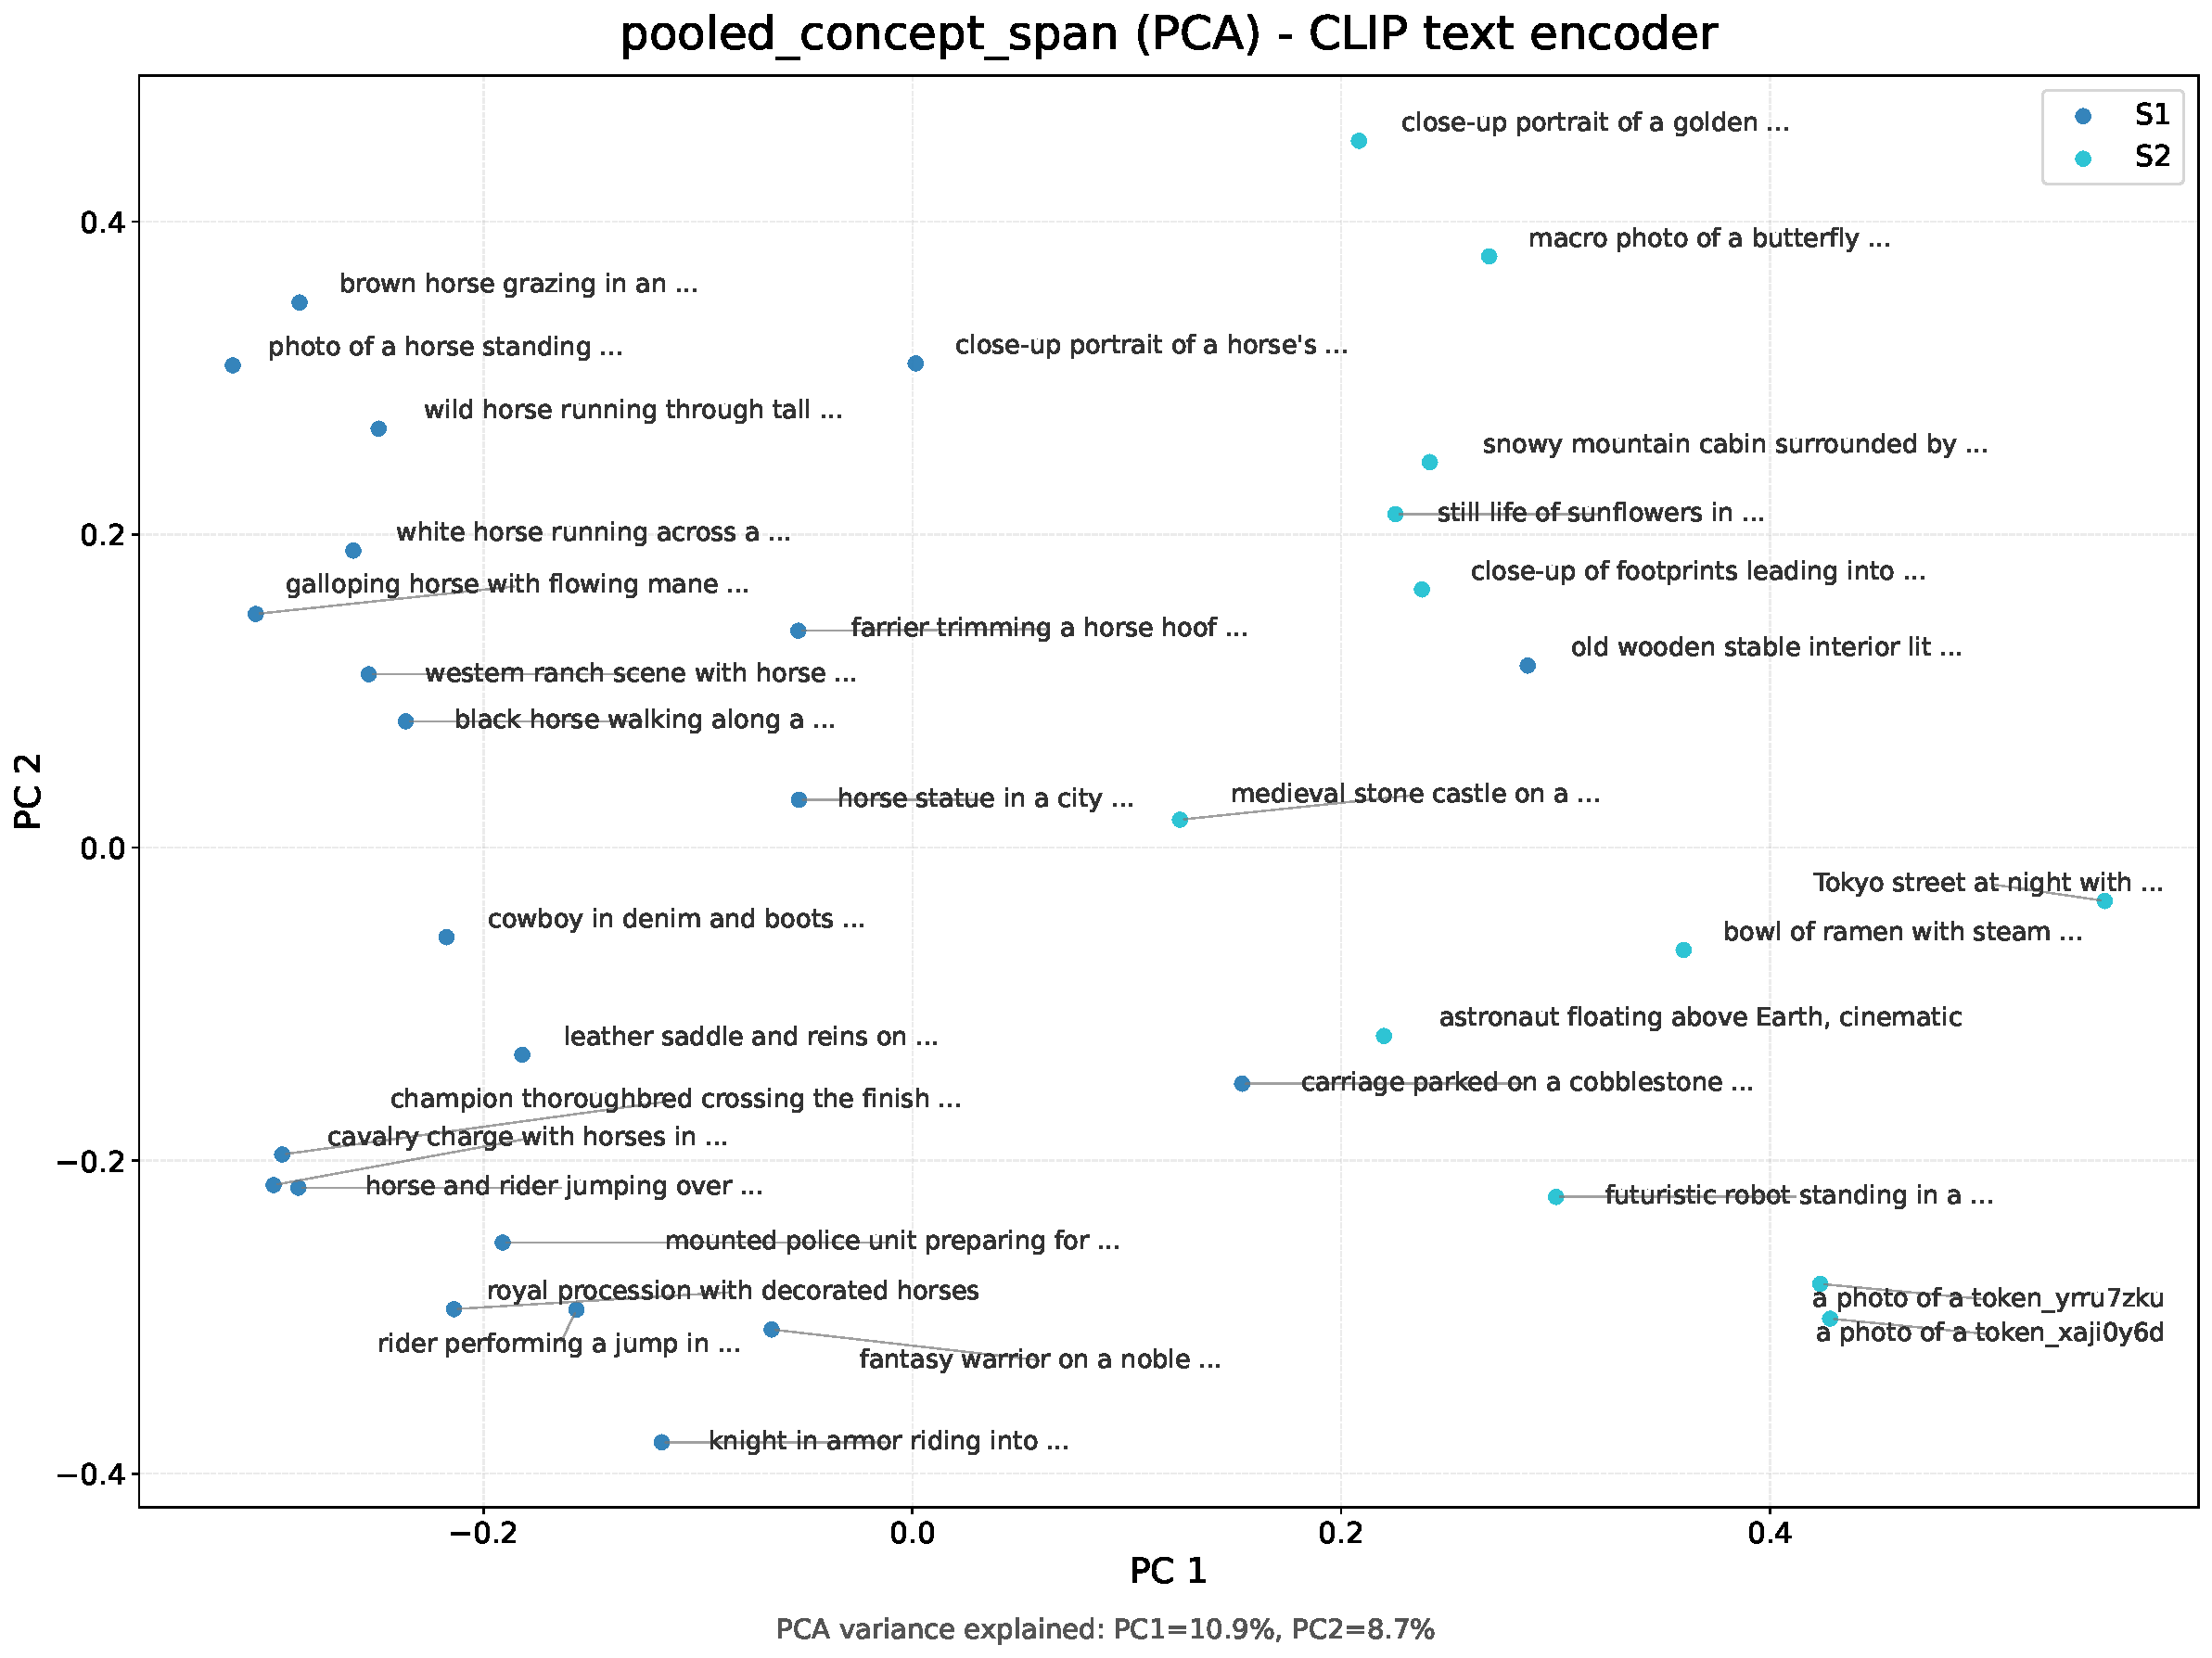
\includegraphics[width=\linewidth]{img/bag_of_words_span.pdf}
\caption{
\textbf{Context-only prompts remain close to target prompts in CLIP text-embedding space.}
PCA projection of pooled prompts used for the \texttt{horse} case study. One group explicitly contains the concept token, while the other omits it but retains correlated context words (e.g., \texttt{jockey}, \texttt{saddle}, \texttt{racetrack}). The proximity between these groups illustrates why token-level erasure can remain vulnerable to indirect contextual prompts.
}
\label{fig:bow_context_span}
\end{figure}


\paragraph{Indirect recovery prompts.}
We use the correlated context set for $c$ to construct a set of indirect prompts $\mathcal{P}_{\mathrm{ind}}(c)$. These prompts are generated under an explicit lexical exclusion constraint: they must not contain the target token or excluded lexical variants of $c$. Intuitively, $\mathcal{P}_{\mathrm{ind}}(c)$ probes whether the erased concept can still be elicited through contextual associations alone, without direct lexical mention. To improve prompt diversity while preserving control, we generate multiple prompts from different subsets of the correlated context words and retain only prompts that satisfy the exclusion rule.

\paragraph{Semantic neighbors and control concepts.}
The semantic neighborhood $\mathcal{N}(c)$ is determined by the universal-pool $\delta$-threshold procedure given in~\cref{def:semantic_neighborhood}: $\mathcal{N}(c)$ collects all candidates in the shared pool $\mathcal{C}_{\mathrm{pool}}$ whose centroid cosine distance to $c$ falls below the global 25th-percentile threshold $\delta$. This produces concept-specific neighborhoods of five to seven discovered neighbors per target (\cref{tab:kappa_per_target}).
The control set $\mathcal{C}(c) = \{\texttt{airplane}, \texttt{bicycle}, \texttt{cactus}, \texttt{jellyfish}, \texttt{lighthouse}, \texttt{melon}, \texttt{police car}, \texttt{teapot}, \texttt{violin}, \texttt{volcano}\}$ is identical across all five targets and consists of concepts whose centroids lie well above $\delta$ for every target, verified to contribute zero to $\hat\kappa$ across all five targets. For each neighbor $c' \in \mathcal{N}(c)$ and control $\tilde c \in \mathcal{C}(c)$, we generate prompts that explicitly mention the concept while excluding lexical forms of the target $c$. Per-target prompt files are released in the supplementary material.

\paragraph{Classifier-based scoring.}
All images are classified using a CLIP-based classifier over a fixed vocabulary of 65 concept labels (\cref{app:vocab}). For each image, the classifier returns the top-1 label among the vocabulary. All metrics defined below are computed from these top-1 assignments. In several random instances, we also perform a manual evaluation to ensure consistency of the results.

% For each prompt set, we generate images from the base model $\mathcal{D}_\theta$ and each unlearned model $\mathcal{D}_{\hat{\theta}}$, and evaluate the outputs using a pretrained concept classifier. For indirect prompts, we measure the fraction of generated images classified as the erased concept $c$, yielding an estimate of indirect recovery. For neighbor prompts, we measure classifier accuracy on the intended neighbor concept $c'$, which captures neighbor preservation after unlearning. For control prompts, we analogously measure accuracy on the intended non-neighbor control concept. Together, these scores allow us to distinguish target-specific collateral damage on semantic neighbors from broader degradation on unrelated concepts.

\subsection{Evaluation Metrics}
\label{app:metric_defs}
Each metric is defined with respect to a base model 
$\mathcal{D}_\theta$ and an unlearned model 
$\mathcal{D}_{\hat\theta}$. We write $\mathrm{Acc}(\mathcal{D}, c, \mathcal{P})$ for the fraction of images generated by model $\mathcal{D}$ from prompts in set $\mathcal{P}$ that are classified as concept $c$ by the CLIP evaluator.

\paragraph{Erasure metrics (measuring $\varepsilon$).}
These metrics measure how effectively the target concept $c$ is suppressed in the unlearned model.
\begin{itemize}
    \item \emph{Unlearning Accuracy (UA)}: The fraction of images generated from direct prompts $\mathcal{P}_{\mathrm{dir}}(c)$ by $\mathcal{D}_{\hat\theta}$ that 
    are \emph{not} classified as $c$. 
    \begin{equation}
    \label{eq:ua}
    \mathrm{UA}(c) = 1 - \mathrm{Acc}(\mathcal{D}_{\hat\theta}, c, \mathcal{P}_{\mathrm{dir}}(c)).
    \end{equation}
    Higher UA indicates more complete erasure under explicit lexical prompts.
    \item \emph{Indirect Recovery Rate (IRR)}: The fraction of images generated from indirect recovery prompts $\mathcal{P}_{\mathrm{ind}}(c)$ by 
    $\mathcal{D}_{\hat\theta}$ that \emph{are} classified as $c$: 
    \begin{equation}
    \label{eq:irr}
    \mathrm{IRR}(c) = \mathrm{Acc}(\mathcal{D}_{\hat\theta}, c, \mathcal{P}_{\mathrm{ind}}(c)).
    \end{equation}
    Higher IRR indicates greater vulnerability to concept recovery through correlated contextual cues. In contrast to UA, IRR measures the $\varepsilon$-robust erasure property formalized in~\cref{def:robust}.
\end{itemize}

\paragraph{Retention metrics (measuring $\gamma$).}
We measure retention at three levels of granularity:
\begin{itemize}
    \item \emph{In-domain Retain Accuracy (IRA)}: The fraction of images generated from indirect prompts by $\mathcal{D}_{\hat\theta}$ that are classified as a non-target, non-neighbor, non-control concept in the vocabulary. This captures the tendency of an unlearned model to substitute unrelated concepts when indirectly prompted for the erased target.
    %\ali{are we using this metric only for the UnlearnCanvas dataset? if not, this part is confusing and not needed.
    \item \emph{Neighbor Preservation (NP)}: This is our primary trade-off metric. The overlap with remaining concepts is often dominated by the overlap with a few concepts which are mostly semantically similar with the target concept. Therefore, as a proxy metric for utility preservation, we evaluate utility preservation in the semantic neighborhood $\mathcal{N}(c)$ of the target concept (\cref{def:semantic_neighborhood}) and define
    \begin{equation}
    \label{eq:neighbor_pres}
    \mathrm{NP}(c) = \frac{1}{|\mathcal{N}(c)|} \sum_{c' \in \mathcal{N}(c)} \frac{\mathrm{Acc}(\mathcal{D}_{\hat\theta}, c', \mathcal{P}_{\mathrm{dir}}(c'))}
    {\mathrm{Acc}(\mathcal{D}_\theta, c', \mathcal{P}_{\mathrm{dir}}(c'))}.
    \end{equation}
    An NP score of $1.0$ indicates perfect preservation of neighbors after unlearning; lower values indicate proportional collateral damage. The ratio form normalizes out the base-model recognition accuracy, which differs across concepts (and which is generally below 1.0 under a 65-class vocabulary).
    % where $\mathrm{Acc}(\mathcal{D}, c')$ denotes classifier accuracy on prompts for concept $c'$ under model $M$. An NP score of 1.0 indicates perfect preservation of nearby concepts, while lower values indicate stronger collateral damage. Unlike IRA, which averages over all non-target concepts, NP focuses specifically on semantically nearby concepts that are most likely to overlap with the erased target. \textbf{Relation to $\gamma$.} NP is an operational, classifier-based proxy for the activation-level neighbor preservation error $\gamma$ in Definition~\ref{def:neighbor}. By Assumption~\ref{asm:lip}, a small activation displacement $\|\Phi_{\hat\theta}(p) - \Phi_\theta(p)\|_2$ induces a small change in concept generation probability and hence a small drop in classifier accuracy; conversely, a method that preserves $\mathrm{NP} \approx 1$ must have kept activations close in $\mathcal{H}$. NP and $1-\gamma$ therefore track the same underlying quantity up to the Lipschitz constant $L$ and classifier noise, which is what makes it the right axis against which to plot Theorem~\ref{thm:tradeoff}'s predicted Pareto frontier.
    \item \emph{Control preservation (CP)}: To distinguish neighbor-specific collateral damage from broader degradation, we additionally evaluate performance on a non-neighbor control set $\mathcal{C}(c)$. We define
    \begin{equation}
    \label{eq:cp}
    \mathrm{CP}(c) = \frac{1}{|\mathcal{C}(c)|} \sum_{\tilde c \in \mathcal{C}(c)} 
    \frac{\mathrm{Acc}(\mathcal{D}_{\hat\theta}, \tilde c, \mathcal{P}_{\mathrm{dir}}(\tilde c))}
     {\mathrm{Acc}(\mathcal{D}_\theta, \tilde c, \mathcal{P}_{\mathrm{dir}}(\tilde c))}.
    \end{equation}
    Comparing NP and CP isolates neighbor-specific collateral damage from broader degradation: a method with $\mathrm{NP} \ll \mathrm{CP}$ is damaging concepts selectively in the target's neighborhood, consistent with the propagation mechanism in~\cref{thm:tradeoff}. A method with $\mathrm{NP} \approx \mathrm{CP} \ll 1$ is causing uniform degradation across the concept space.
    % where $\tilde{c}$ denotes a control concept that is semantically distant from $c$. Comparing NP and CP allows us to determine whether a method disproportionately harms nearby concepts, rather than causing uniform degradation across the concept space.
\end{itemize}


% \paragraph{Image quality.}
% We report Fr'{e}chet Inception Distance (FID)~\citep{heusel2017gans} to verify that the observed tradeoffs are not merely artifacts of overall image-quality degradation.


\paragraph{DamageGap.} A summary statistic we introduce to quantify neighbor-selective damage: $\mathrm{DamageGap}(c) = \mathrm{CP}(c) - \mathrm{NP}(c)$. A positive DamageGap indicates that neighbors are damaged more than controls, consistent with the trade-off predicted by~\cref{thm:tradeoff}. A DamageGap near zero indicates uniform degradation (or uniform preservation) across both sets.

\subsection{Classification Vocabulary}
\label{app:vocab}
All CLIP-based classification uses the following 65-concept vocabulary, which is identical to the universal candidate pool $\mathcal{C}_{\mathrm{pool}}$ used for $\hat\kappa$ estimation (\cref{app:kappa_estimation}).
The same vocabulary is used for every metric and every target, ensuring cross-target comparability.

\begin{table}[h]
\centering
\small
\begin{tabular}{p{3.2cm} p{10cm}}
\toprule
Category & Concepts \\
\midrule
Targets & \texttt{horse}, \texttt{cat}, \texttt{dog}, \texttt{bear}, \texttt{castle} \\
Equine  & \texttt{pony}, \texttt{donkey}, \texttt{zebra}, \texttt{mustang}, \texttt{mare}, \texttt{foal}, \texttt{stallion}, \texttt{mule}, \texttt{bison}, \texttt{camel} \\
Feline  & \texttt{kitten}, \texttt{tiger}, \texttt{lion}, \texttt{leopard}, \texttt{panther}, \texttt{cheetah}, \texttt{lynx}, \texttt{jaguar}, \texttt{cougar}, \texttt{bobcat} \\
Canid  & \texttt{puppy}, \texttt{fox}, \texttt{coyote}, \texttt{jackal}, \texttt{dingo}, \texttt{hyena}, \texttt{husky}, \texttt{labrador}, \texttt{beagle}, \texttt{retriever} \\
Ursine & \texttt{grizzly}, \texttt{polar bear}, \texttt{panda}, \texttt{cub}, \texttt{koala}, \texttt{black bear}, \texttt{brown bear}, \texttt{teddy bear}, \texttt{sloth bear}, \texttt{sun bear} \\
Architectural  & \texttt{fortress}, \texttt{tower}, \texttt{cathedral}, \texttt{palace}, \texttt{keep}, \texttt{citadel}, \texttt{watchtower}, \texttt{stronghold}, \texttt{fortified wall}, \texttt{manor} \\
Controls  & \texttt{airplane}, \texttt{bicycle}, \texttt{cactus}, \texttt{jellyfish}, \texttt{lighthouse}, \texttt{melon}, \texttt{police car}, \texttt{teapot}, \texttt{violin}, \texttt{volcano} \\
\bottomrule
\end{tabular}
\caption{The $65$-concept classification vocabulary used for all CLIP-based metric evaluations in~\cref{sec:experiment}. The vocabulary is the union of the five targets, their respective fine-grained subtype candidates spanning four animal category and one architectural category, and ten out-of-domain controls. See~\cref{tab:kappa_per_target} for the per-target subset $\mathcal{N}(c) \subseteq \mathcal{C}_{\mathrm{pool}}$ that survives the $\delta$-filter and forms the averaging set for NP.}
\label{tab:vocab}
\end{table}

\section{Per-Concept Results}
\label{app:per_concept_tables}

This appendix provides the per-concept evaluation tables underlying the averaged results in \Cref{tab:main_results_avg}. For each of the five target concepts, we report all metrics across the seven unlearning methods. The concepts span estimated entanglement coefficients $\hat\kappa \in [0.27, 0.89]$ (\Cref{tab:kappa}), enabling the $\kappa$-scaling analysis in \Cref{subsec:kappa_scaling}.

We order tables by $\hat\kappa$ in descending order to make the predicted scaling visually apparent: collateral damage (low IRA, low NP, high DamageGap) is most pronounced for high-$\hat\kappa$ concepts and attenuates as $\hat\kappa$ decreases.

\paragraph{SAeUron coverage.} 
SAeUron's released sparse autoencoder features cover the four animal concepts (\texttt{dog}, \texttt{bear}, \texttt{horse}, \texttt{cat}) but not \texttt{castle}. We mark the corresponding row with -- in \Cref{tab:per_concept_castle} and exclude SAeUron from the averaged castle entries. Attempts to substitute SAeUron's \texttt{architectures} feature for \texttt{castle} did not yield meaningful suppression of castle generation (verified by visual inspection at the default ablation multiplier); we therefore report SAeUron only on concepts where its released features apply.

\paragraph{Reading the tables.}
All tables follow the same column structure as \Cref{tab:main_results_avg}: erasure metrics (UA, IRR), retention metrics (IRA, NP, CP), and the composite DamageGap. The \emph{Original} row reports baseline rates for the unedited $\mathcal{D}_\theta$ on each concept's evaluation set; note that baseline IRA varies substantially across concepts (e.g., {0.85} for \texttt{cat} vs. {0.54} for \texttt{tower/castle}) due to differences in CLIP evaluator accuracy on each concept's in-domain object set. This per-concept baseline variation motivates our use of normalized retention ratios in~\cref{subsec:kappa_scaling}.

% ============================================================
% Per-concept tables, ordered by descending kappa
% ============================================================

\subsection{Dog}
\label{app:per_concept_dog}

\begin{table}[ht]
\centering
\small
\setlength{\tabcolsep}{5pt}
\begin{tabular}{llcccccc}
\toprule
& & \multicolumn{2}{c}{\textbf{Erasure}} & \multicolumn{3}{c}{\textbf{Retention}} & \\
\cmidrule(lr){3-4} \cmidrule(lr){5-7}
\textbf{Method} & \textbf{Type} & UA$\uparrow$ & IRR$\downarrow$ & IRA$\uparrow$ & NP$\uparrow$ & CP$\uparrow$ & DamageGap$\downarrow$ \\
\midrule
Original    & --          & 0     & 27.0  & 78.92 & 100   & 100   & --    \\
\midrule
ESD         & FT          & 75.0  & 17.5  & 74.15 & 93.51 & 96.0  & 2.48  \\
SalUn       & FT          & 90.0  & 8.0   & 50.92 & 58.01 & 76.0  & 17.98 \\
EDiff       & FT          & 62.0  & 23.5  & 66.61 & 80.29 & 92.99 & 12.70 \\
\midrule
AdvUnlearn  & Robust FT   & 96.0  & 20.0  & 74.30 & 63.05 & 99.0  & 35.94 \\
STEREO      & Robust FT   & 100.0 & 1.0   & 4.76  & 1.81  & 64.0  & 62.18 \\
\midrule
SEOT        & Inf.        & 68.0  & 30.0  & 79.07 & 84.20 & 99.0  & 14.80 \\
SAeUron     & Inf.        & 78.0  & 18.5  & 8.76  & 4.27  & 73.0  & 68.72 \\
\bottomrule
\end{tabular}
\caption{\textbf{Per-concept evaluation for \texttt{dog} ($\hat\kappa = 0.89$).} Discovered neighbors include 
\texttt{puppy}, \texttt{labrador}, \texttt{beagle}, \texttt{husky}, and \texttt{retriever} (full list in~\Cref{app:eval_pipeline}). As the highest-$\hat\kappa$ concept in our evaluation, \texttt{dog} exhibits the most severe robustness--retention trade-off: robust fine-tuning methods (STEREO, AdvUnlearn) achieve high UA but cause substantial IRA and NP degradation.}
\label{tab:per_concept_dog}
\end{table}

\paragraph{Observations.}
\texttt{Dog} exhibits the most severe trade-off in our evaluation, consistent with its position as the highest-$\hat\kappa$ concept. STEREO achieves complete erasure (UA = $100$) but collapses NP to $1.81$ and IRA to $4.76$ --- effectively destroying the model's ability to generate dog-related neighbors. SAeUron shows analogous catastrophic damage (NP = $4.27$, IRA = $8.76$) despite operating at inference time, suggesting that even modest displacement can wreck retention when neighbor activation regions densely overlap the target. ESD stands out as the only method achieving meaningful erasure (UA = $75$) while preserving neighbors well (NP = $93.51$, DamageGap = $2.48$), at the cost of higher residual leakage (IRR = $17.5$). The Pareto separation between ESD ($75, 93.51$) and STEREO ($100, 1.81$) is a $\approx 92$-point NP gap for a $25$-point UA gain, the steepest trade-off observed across our concepts and a direct empirical instantiation of the $\kappa$-scaled lower bound predicted by~\Cref{thm:tradeoff}.

% ------------------------------------------------------------

\subsection{Bear}
\label{app:per_concept_bear}

\begin{table}[ht]
\centering
\small
\setlength{\tabcolsep}{5pt}
\begin{tabular}{llcccccc}
\toprule
& & \multicolumn{2}{c}{\textbf{Erasure}} & \multicolumn{3}{c}{\textbf{Retention}} & \\
\cmidrule(lr){3-4} \cmidrule(lr){5-7}
\textbf{Method} & \textbf{Type} & UA$\uparrow$ & IRR$\downarrow$ & IRA$\uparrow$ & NP$\uparrow$ & CP$\uparrow$ & DamageGap$\downarrow$ \\
\midrule
Original    & --          & 0     & 85.5  & 62.75 & 100   & 100   & --    \\
\midrule
ESD         & FT          & 94.5  & 9.0   & 44.00 & 58.02 & 95.0  & 36.97 \\
SalUn       & FT          & 99.5  & 5.5   & 51.51 & 53.89 & 89.0  & 35.10 \\
EDiff       & FT          & 96.0  & 6.0   & 38.61 & 56.75 & 94.0  & 37.24 \\
\midrule
AdvUnlearn  & Robust FT   & 99.0  & 1.0   & 42.46 & 67.37 & 100   & 32.62 \\
STEREO      & Robust FT   & 99.5  & 2.0   & 15.88 & 13.75 & 77.0  & 63.25 \\
\midrule
SEOT        & Inf.        & 94.0  & 13.5  & 50.84 & 64.14 & 96.48 & 32.34 \\
SAeUron     & Inf.        & 85.5  & 15.0  & 22.37 & 63.50 & 93.8  & 30.30 \\
\bottomrule
\end{tabular}
\caption{\textbf{Per-concept evaluation for \texttt{bear} ($\hat\kappa = 0.82$).} Discovered neighbors include \texttt{grizzly}, \texttt{panda}, \texttt{polar bear}, \texttt{koala}, and \texttt{cub} (full list in~\Cref{app:eval_pipeline}).}
\label{tab:per_concept_bear}
\end{table}

\paragraph{Observations.}
\texttt{Bear} sits in the high-$\hat\kappa$ regime alongside horse and dog, and exhibits the predicted Pareto structure. STEREO again occupies the high-erasure / low-retention extreme (UA = $99.5$, NP = $13.75$, DamageGap = $63.25$), while AdvUnlearn achieves comparable erasure (UA = $99$) with substantially better neighbor preservation (NP = $67.37$). The clustering pattern is unusually compressed on bear: standard fine-tuning methods (ESD, SalUn, EDiff) and the inference-time methods cluster tightly between NP = $53.89$--$67.37$, with SEOT and AdvUnlearn essentially tied at NP $\approx 64$--$67$. Notably, no method on bear matches the (high UA, high NP) operating point achieved on lower-$\hat\kappa$ concepts: even ESD, the best performer on \texttt{dog} and \texttt{castle}, reaches only NP = $58.02$ here. This compression of the achievable retention region is a direct manifestation of the $\hat\kappa$-scaled Pareto frontier predicted by~\Cref{thm:tradeoff}.
\subsection{Horse}
\label{app:per_concept_horse}

\begin{table}[ht]
\centering
\small
\setlength{\tabcolsep}{5pt}
\begin{tabular}{llcccccc}
\toprule
& & \multicolumn{2}{c}{\textbf{Erasure}} & \multicolumn{3}{c}{\textbf{Retention}} & \\
\cmidrule(lr){3-4} \cmidrule(lr){5-7}
\textbf{Method} & \textbf{Type} & UA$\uparrow$ & IRR$\downarrow$ & IRA$\uparrow$ & NP$\uparrow$ & CP$\uparrow$ & DamageGap$\downarrow$ \\
\midrule
Original    & --          & 0     & 75.5  & 71.23 & 100   & 100   & --    \\
\midrule
ESD         & FT          & 80.0  & 33.5  & 62.92 & 81.12 & 97.0  & 15.87 \\
SalUn       & FT          & 95.0  & 28.5  & 40.92 & 39.42 & 91.99 & 52.57 \\
EDiff       & FT          & 81.0  & 31.0  & 63.84 & 76.48 & 94.0  & 17.51 \\
\midrule
AdvUnlearn  & Robust FT   & 97.5  & 23.0  & 65.38 & 71.42 & 100   & 28.57 \\
STEREO      & Robust FT   & 100.0 & 7.5   & 20.74 & 14.71 & 27.0  & 12.28 \\
\midrule
SEOT        & Inf.        & 81.5  & 38.5  & 69.69 & 97.06 & 99.0  & 1.93  \\
SAeUron     & Inf.        & 78.0  & 39.5  & 76.92 & 82.48 & 94.0  & 11.51 \\
\bottomrule
\end{tabular}
\caption{\textbf{Per-concept evaluation for \texttt{horse} ($\hat\kappa = 0.81$).} Discovered neighbors include 
\texttt{pony}, \texttt{mare}, \texttt{donkey}, \texttt{zebra}, \texttt{stallion}, \texttt{foal} and \texttt{mule} (full list in~\Cref{app:eval_pipeline}).}
\label{tab:per_concept_horse}
\end{table}

\paragraph{Observations.}
\texttt{Horse} is the running example used throughout \Cref{sec:experiment} and exhibits the canonical Pareto structure across method families. STEREO occupies the high-erasure / catastrophic-retention extreme (UA = $100$, NP = $14.71$, IRA = $20.74$); SEOT and SAeUron occupy the high-retention / weaker-erasure region (NP $\geq 82$ but IRR $\geq 38.5$); standard fine-tuning methods sit in between, with ESD reaching a clean $(80, 81.12)$ operating point at DamageGap = $15.87$. SalUn is an outlier among standard FT methods, achieving high UA = $95$ with NP = $39.42$, far below ESD and EDiff at comparable erasure --- consistent with SalUn's gradient-saliency masking displacing more activation than necessary for erasure. A second notable observation is STEREO's collapsed CP = $27$, far below STEREO's CP on the other four concepts (range $64$--$96$): in this high-$\hat\kappa$ regime, STEREO's adversarial subspace appears to spill beyond the intended object subspace into stylistically-correlated features, manifesting the broad subspace suppression discussed in~\Cref{rem:stereo}.
\subsection{Cat}
\label{app:per_concept_cat}

\begin{table}[ht]
\centering
\small
\setlength{\tabcolsep}{5pt}
\begin{tabular}{llcccccc}
\toprule
& & \multicolumn{2}{c}{\textbf{Erasure}} & \multicolumn{3}{c}{\textbf{Retention}} & \\
\cmidrule(lr){3-4} \cmidrule(lr){5-7}
\textbf{Method} & \textbf{Type} & UA$\uparrow$ & IRR$\downarrow$ & IRA$\uparrow$ & NP$\uparrow$ & CP$\uparrow$ & DamageGap$\downarrow$ \\
\midrule
Original    & --          & 0     & 96.0  & 85.50 & 100   & 100   & --    \\
\midrule
ESD         & FT          & 66.0  & 38.0  & 66.92 & 87.35 & 98.0  & 0.80  \\
SalUn       & FT          & 87.0  & 21.0  & 34.53 & 73.04 & 100   & 26.95 \\
EDiff       & FT          & 76.0  & 24.0  & 62.30 & 65.99 & 100   & 34.00 \\
\midrule
AdvUnlearn  & Robust FT   & 100.0 & 0.0   & 50.76 & 72.40 & 98.0  & 25.60 \\
STEREO      & Robust FT   & 93.0  & 7.0   & 27.68 & 27.60 & 90.0  & 62.40 \\
\midrule
SEOT        & Inf.        & 71.66 & 34.0  & 42.15 & 81.99 & 100   & 18.01 \\
SAeUron     & Inf.        & 72.0  & 37.5  & 60.25 & 85.63 & 96.0  & 10.37 \\
\bottomrule
\end{tabular}
\caption{\textbf{Per-concept evaluation for \texttt{cat} ($\hat\kappa = 0.77$).} Discovered neighbors include \texttt{kitten}, \texttt{lynx}, \texttt{leopard}, \texttt{tiger}, and \texttt{cheetah} (full list in~\Cref{app:eval_pipeline}). The original baseline IRA = $85.50$ reflects high CLIP-evaluator accuracy on cat's in-domain object set after correcting for kitten/cat label confusion (see~\Cref{app:evaluation_setup}).}
\label{tab:per_concept_cat}
\end{table}

\paragraph{Observations.}
\texttt{Cat} exhibits a trade-off structure consistent with the high-$\hat\kappa$ regime, though its base IRA = $85.50$ is the highest of the five concepts, providing more retention "headroom" than other targets. STEREO again occupies the high-erasure / catastrophic-retention extreme (UA = $93$, NP = $27.60$, IRA = $27.68$), with DamageGap = $62.40$ matching its damage on horse and bear. AdvUnlearn achieves complete erasure (UA = $100$, IRR = $0$) at NP = $72.40$, demonstrating that adversarial training can preserve neighbors more effectively than STEREO at comparable erasure strength. ESD achieves a notable operating point: UA = $66$ at NP = $87.35$ with DamageGap = $0.80$, the cleanest standard-FT result on any concept in our evaluation, though at the cost of higher residual leakage (IRR = $38$). The STEREO IRA-retention ratio for cat ($27.68 / 85.50 = 0.32$) is consistent with the corresponding ratio on horse ($0.29$) and bear ($0.25$), reinforcing the $\hat\kappa$-scaling result in~\Cref{subsec:kappa_scaling}.
\subsection{Castle}
\label{app:per_concept_castle}

\begin{table}[ht]
\centering
\small
\setlength{\tabcolsep}{5pt}
\begin{tabular}{llcccccc}
\toprule
& & \multicolumn{2}{c}{\textbf{Erasure}} & \multicolumn{3}{c}{\textbf{Retention}} & \\
\cmidrule(lr){3-4} \cmidrule(lr){5-7}
\textbf{Method} & \textbf{Type} & UA$\uparrow$ & IRR$\downarrow$ & IRA$\uparrow$ & NP$\uparrow$ & CP$\uparrow$ & DamageGap$\downarrow$ \\
\midrule
Original    & --          & 0     & 9.5   & 53.84 & 100   & 100   & --    \\
\midrule
ESD         & FT          & 88.0  & 6.5   & 48.15 & 83.03 & 99.0  & 15.98 \\
SalUn       & FT          & 97.0  & 1.0   & 54.76 & 67.58 & 94.0  & 26.41 \\
EDiff       & FT          & 82.0  & 2.5   & 46.46 & 87.35 & 99.0  & 18.69 \\
\midrule
AdvUnlearn  & Robust FT   & 100.0 & 1.0   & 44.00 & 83.10 & 100   & 16.89 \\
STEREO      & Robust FT   & 100.0 & 0.0   & 29.38 & 31.96 & 96.0  & 64.03 \\
\midrule
SEOT        & Inf.        & 98.0  & 6.5   & 53.84 & 98.21 & 99.0  & 0.79  \\
SAeUron     & Inf.        & --    & --    & --    & --    & --    & --    \\
\bottomrule
\end{tabular}
\caption{\textbf{Per-concept evaluation for \texttt{castle} ($\hat\kappa = 0.27$).} Discovered neighbors include 
\texttt{fortress}, \texttt{palace}, \texttt{citadel}, \texttt{keep}, \texttt{cathedral} and \texttt{manor} (full list in~\Cref{app:eval_pipeline}). SAeUron's released sparse autoencoder features do not cover \texttt{castle}; we attempted to substitute its \texttt{architectures} feature, but the resulting ablation did not yield meaningful suppression of castle generation.}
\label{tab:per_concept_castle}
\end{table}

\paragraph{Observations.}
\texttt{Castle} is the lowest-$\hat\kappa$ concept in our evaluation and demonstrates qualitatively different trade-off behavior from the high-$\hat\kappa$ animal concepts. Several methods achieve strong erasure with minimal retention damage: ESD reaches UA = $88$ at NP = $83.03$ (DamageGap = $15.98$), AdvUnlearn achieves complete erasure (UA = $100$) at NP = $83.10$ (DamageGap = $16.89$), and SEOT reaches UA = $98$ at NP = $98.21$ (DamageGap = $0.79$, the lowest of any (method, concept) pair in our evaluation). This is qualitatively distinct from the high-$\hat\kappa$ concepts, where no method achieves both UA $\geq 90$ and NP $\geq 80$. STEREO is the notable exception: despite the low predicted $\kappa$-floor, STEREO incurs NP = $31.96$ and DamageGap = $64.03$, comparable to its damage on the high-$\hat\kappa$ animal concepts. This is the empirical illustration of \Cref{thm:tradeoff} as a \emph{lower bound} rather than a ceiling: STEREO's REO objective broadly suppresses the spanned adversarial subspace regardless of whether neighbors actually occupy the displaced region (\Cref{rem:stereo}), producing damage well above the $\kappa$-predicted floor that other methods successfully hug. The separation between STEREO and the alternatives on \texttt{castle} suggests room for $\kappa$-aware unlearning methods that achieve robust erasure without STEREO's $\kappa$-blind over-suppression.

\section{Direct Validation: Activation Displacement Scales with $\hat\kappa$}
\label{app:displacement_kappa}
\Cref{thm:tradeoff} predicts that activation displacement at neighbor prompts scales linearly with $\kappa$ for a method achieving $\varepsilon$-robust erasure. The Neighbor Preservation (NP) measure used in~\Cref{sec:experiment} is a probability-units proxy for this displacement, related through~\cref{asm:lip}. To test~\Cref{thm:tradeoff}'s prediction in the units the theorem is stated in, we measure activation displacement directly:
\[
\Delta_{\text{neighbor}}(c_u) \;=\; \mathbb{E}_{p_{c'} \sim \mathcal{N}_\delta(c_u)}\!\left[\, \big\| \Phi_{\hat\theta}(p_{c'}) - \Phi_\theta(p_{c'}) \big\|_2 \,\right]
\]
% We measure $\Delta_{\text{neighbor}}$ for each fine-tuning method on each of the five target concepts using $200$ neighbor prompts per concept, with activations captured from \texttt{up\_blocks.1.attentions.1} at DDIM step $25$ of $50$. Inference-time methods are omitted: SEOT's text-embedding intervention does not propagate measurably to this layer in $L_2$ distance, and SAeUron's sparse-feature ablation produces displacement values an order of magnitude larger than fine-tuning methods, reflecting a real mechanism difference rather than direct comparability with weight-update methods.
We measure $\Delta_{\text{neighbor}}$ for each fine-tuning method on each of the five target concepts using $200$ neighbor prompts per concept, with activations captured from \texttt{up\_blocks.1.attentions.1} at DDIM step $25$ of $50$. Activations are flattened across spatial and token dimensions before computing $L_2$ distances, so absolute magnitudes here are larger than the mean-pooled token-level magnitudes reported in~\cref{app:displacement} (\cref{fig:displacement}); both views are consistent in ordering and in the prediction they probe (within-target ordering in~\cref{app:displacement}, cross-target $\hat\kappa$-scaling here). Inference-time methods are omitted: SEOT's text-embedding intervention does not propagate measurably to this layer in $L_2$ distance, and SAeUron's sparse-feature ablation produces displacement values an order of magnitude larger than fine-tuning methods, reflecting a real mechanism difference rather than direct comparability with weight-update methods.

\paragraph{Displacement scales monotonically with $\hat\kappa$.}
\Cref{tab:displacement} reports mean neighbor displacement across the five concepts and five fine-tuning methods. Four of five methods exhibit positive Spearman rank correlation between $\hat\kappa$ and displacement, with ESD showing strict monotonicity ($\rho = +1.00$) and STEREO closely tracking ($\rho = +0.90$ with a single inversion between \texttt{cat} and \texttt{horse}, whose $\hat\kappa$ values differ by only $0.04$). Across all five methods, displacement on \texttt{castle} ($\hat\kappa = 0.27$) is substantially lower than the average displacement across the four high-$\hat\kappa$ animal concepts: ratios range from $1.68\times$ (ESD) to $3.18\times$ (STEREO). The qualitative form predicted by \Cref{thm:tradeoff} --- displacement increasing with $\hat\kappa$ --- is empirically supported.

\begin{table}[h]
\centering
\small
\setlength{\tabcolsep}{6pt}
\begin{tabular}{lccccc|c}
\toprule
\textbf{Method} & \texttt{castle} & \texttt{cat} & \texttt{horse} & \texttt{bear} & \texttt{dog} & Spearman $\rho$ \\
& ($\hat\kappa{=}0.27$) & ($0.77$) & ($0.81$) & ($0.82$) & ($0.89$) & vs.\ $\hat\kappa$ \\
\midrule
ESD        & 128.4 & 194.8 & 213.6 & 221.0 & 235.4 & $+1.00$ \\
STEREO     & \phantom{0}75.9 & 234.2 & 233.4 & 240.9 & 257.0 & $+0.90$ \\
AdvUnlearn & \phantom{0}71.6 & 110.5 & 150.9 & 123.2 & 123.7 & $+0.70$ \\
EDiff      & \phantom{0}67.8 & 163.0 & 178.1 & 172.1 & 175.6 & $+0.70$ \\
SalUn      & \phantom{0}88.1 & 220.7 & 215.6 & 220.4 & 215.3 & $+0.10$ \\
\bottomrule
\end{tabular}
\caption{\textbf{Mean activation displacement at neighbor prompts.} Each cell reports $\Delta_{\text{neighbor}}$ in $L_2$ activation distance, averaged over $200$ neighbor prompts. Spearman $\rho$ is computed across the five concepts. Note that $n = 5$ concepts limits the statistical power of significance testing on individual methods; we report $\rho$ as a descriptive monotonicity measure. The consistency of positive correlations across four of five methods (range $+0.10$ to $+1.00$) provides aggregate evidence for the $\kappa$-scaling predicted by~\Cref{thm:tradeoff}.}
\label{tab:displacement}
\end{table}

\paragraph{STEREO's displacement is consistent with a single local Lipschitz constant.}
\Cref{thm:tradeoff} predicts that for a method operating exactly at the bound, the ratio $\kappa(1-\varepsilon)/(\Delta_{\text{neighbor}} + \delta)$ should equal a single Lipschitz constant $L$ across all concepts. We compute this ratio for each method using STEREO's saturated $\varepsilon \approx 0.035$ (mean IRR across the five concepts; see~\cref{tab:main_results_avg})  and $\delta = 0.05$. The resulting $L_{\text{tight}}$ values are reported in~\Cref{tab:l_tight}. STEREO's $L_{\text{tight}}$ varies by only $7.8\%$ across the five concepts ($L \in [0.0032, 0.0035]$); other methods exhibit spreads of $24\%$ to $57\%$. STEREO's single-$L$ consistency is precisely the quantitative prediction of \Cref{thm:tradeoff}: a method operating at the bound should exhibit a $\kappa$-and-concept-independent local Lipschitz constant. Among the five methods evaluated, only STEREO satisfies this prediction, consistent with STEREO occupying the high-$\Delta$, low-$\varepsilon$ regime where the bound is tightest.

\begin{table}[h]
\centering
\small
\setlength{\tabcolsep}{6pt}
\begin{tabular}{lcccccc}
\toprule
\textbf{Method} & \texttt{castle} & \texttt{cat} & \texttt{horse} & \texttt{bear} & \texttt{dog} & Spread \\
\midrule
\textbf{STEREO} & 0.0035 & 0.0032 & 0.0034 & 0.0033 & 0.0034 & \textbf{7.8\%} \\
EDiff           & 0.0039 & 0.0046 & 0.0045 & 0.0047 & 0.0050 & 23.6\% \\
SalUn           & 0.0030 & 0.0034 & 0.0037 & 0.0036 & 0.0040 & 29.5\% \\
ESD             & 0.0021 & 0.0039 & 0.0037 & 0.0036 & 0.0037 & 53.4\% \\
AdvUnlearn      & 0.0037 & 0.0068 & 0.0053 & 0.0065 & 0.0070 & 57.1\% \\
\bottomrule
\end{tabular}
\caption{\textbf{Per-concept $L_{\text{tight}}$ values.} $L_{\text{tight}} = \kappa(1-\varepsilon)/(\Delta_{\text{neighbor}} + \delta)$ is the Lipschitz constant value that places \Cref{thm:tradeoff}'s bound exactly at the observed displacement. If a method operates at the bound, $L_{\text{tight}}$ should be approximately constant across concepts. STEREO is the only method exhibiting this consistency ($7.8\%$ spread), supporting its operation at the bound's saturated-erasure regime.}
\label{tab:l_tight}
\end{table}

\paragraph{Local versus global Lipschitz.}
The local $L \approx 0.0034$ inferred from STEREO's displacement is much smaller than the global $\hat L = 0.174$ reported in~\Cref{fig:lipschitz}. This reflects the well-known phenomenon that probability changes saturate near classification decision boundaries: the global Lipschitz constant measured across diverse prompt-pair perturbations averages over both saturated and unsaturated regimes, while the local constant near $\mathcal{R}_{c_u}$ during erasure reflects unsaturated behavior specifically. The two values are compatible measurements of different but related quantities; principled estimation of $L$ that distinguishes these regimes is a direction for future work.
% \paragraph{Hierarchical metrics (for style experiments).}
% For style unlearning experiments, we additionally report:
% \begin{itemize}
% \item \emph{Parent Reversion Rate (PRR)}: the fraction of images generated from prompts targeting an erased child style $S_{\mathrm{child}}$ that are classified as either the parent style $S_{\mathrm{parent}}$ or a sibling style $S_{\mathrm{sibling}}$. A PRR substantially above the base rate indicates structured reversion toward nearby styles rather than random degradation.
% \end{itemize}

\newpage
\section{New Baselines}
\begin{table}[htbp]
\centering
\caption{\textbf{Additional baseline comparisons.}
    This table extends the averaged comparison in~\Cref{tab:main_results_avg}
    with five newly evaluated baselines: UCE~\citep{gandikota2024unified}, RECE~\citep{gong2024reliable}, CPE~\citep{lee2025concept}, TRUST~\citep{kori2026selective}, SLD~\citep{schramowski2023safe}, and SAFREE~\citep{yoon2025safree}.
    Methods are grouped by intervention type: closed-form, fine-tuning,
    or inference-time. Cells report mean $\pm$ standard deviation across
    the evaluated target concepts, using the same erasure and retention
    metrics as the main table. The \emph{Original} row denotes the
    unedited-model reference for this comparison.}
\resizebox{\textwidth}{!}{%
\begin{tabular}{llcccccc}
\toprule
& & \multicolumn{2}{c}{\textbf{Erasure}} & \multicolumn{3}{c}{\textbf{Retention}} & \\
\cmidrule(lr){3-4} \cmidrule(lr){5-7}
\textbf{Method} & \textbf{Type} & UA$\uparrow$ & IRR$\downarrow$ & IRA$\uparrow$ & NP$\uparrow$ & CP$\uparrow$ & DamageGap$\downarrow$ \\
\midrule
uCE    & Closed-form & $80.6 \pm 18.4$ & $10.5 \pm 23.4$ & $67.1 \pm 12.4$ & $88.6 \pm 25.1$ & $99.3 \pm 3.1$  & $10.7 \pm 25.4$ \\
RECE   & Closed-form & $99.4 \pm 0.9$  & $3.0 \pm 4.0$   & $43.3 \pm 12.1$ & $56.1 \pm 10.6$  & $93.5 \pm 2.0$  & $37.4 \pm 10.2$ \\
\midrule
CPE    & FT          & $99.6 \pm 0.9$  & $4.7 \pm 9.4$   & $53.4 \pm 12.4$ & $71.9 \pm 18.1$  & $99.6 \pm 2.6$ & $18.7 \pm 19.3$ \\
TRUST    & FT          & $94.2 \pm 2.2$  & $6.5 \pm 3.5$   & $53.2 \pm 13.7$ & $76.4 \pm 9.1$  & $98.0 \pm 5.0$ & $11.6 \pm 12.2$ \\
\midrule
SLD    & Inf. & $99.6 \pm 0.9$  & $0.5 \pm 0.9$   & $35.0 \pm 8.1$  & $58.8 \pm 16.8$  & $89.1 \pm 4.1$  & $30.3 \pm 16.3$ \\
SAFREE & Inf. & $91.4 \pm 11.4$ & $8.4 \pm 10.2$  & $39.9 \pm 8.6$  & $64.7 \pm 16.0$  & $85.7 \pm 12.2$ & $21.0 \pm 19.4$ \\
\bottomrule
\end{tabular}%
    }
    \label{tab:additional_baselines}
\end{table}

\begin{figure}[htbp]
\centering
\begin{minipage}[c]{0.45\linewidth}
\centering
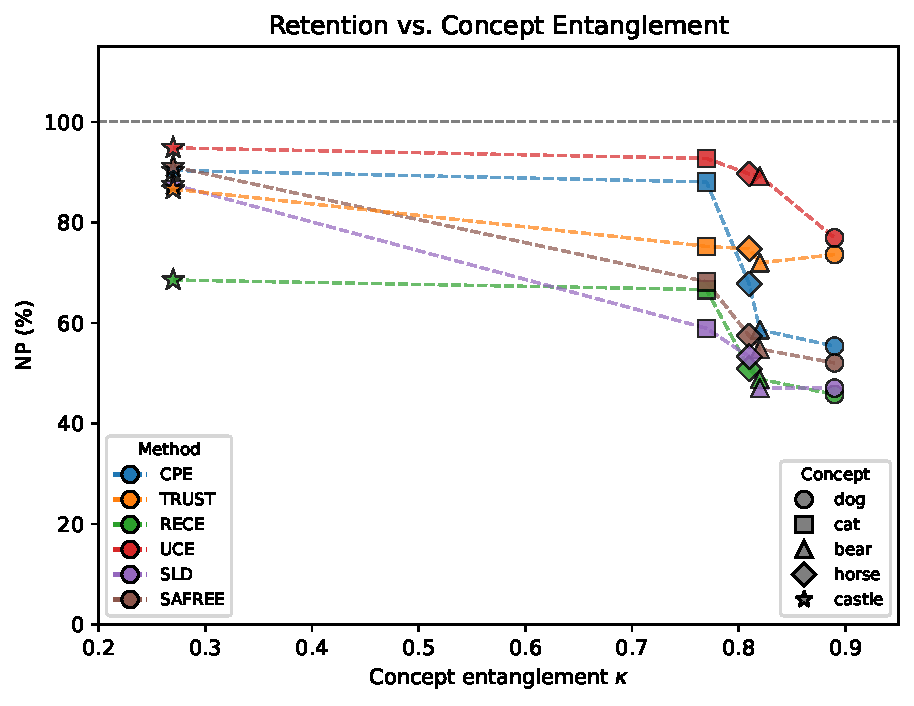
\includegraphics[width=\linewidth]{img/pareto_new_baselines_ua_only.pdf}
\end{minipage}\hfill
\begin{minipage}[c]{0.45\linewidth}
\centering
\scriptsize
\setlength{\tabcolsep}{5pt}
\begin{tabular}{lccc}
\toprule
\textbf{Concept} & $\hat\kappa$ & NP$\uparrow$ & IRA-ratio$\uparrow$ \\
\midrule
\texttt{castle} & 0.27 & 86.47 & 0.79 \\
\texttt{cat}    & 0.77 & 74.88 & 0.78 \\
\texttt{horse}  & 0.81 & 62.54 & 0.74 \\
\texttt{bear}   & 0.82 & 59.71 & 0.70 \\
\texttt{dog}    & 0.89 & 56.58 & 0.65 \\
\midrule
\multicolumn{2}{l}{Spearman $\rho$} & $-1.0$ & $-1.0$ \\
\bottomrule
\end{tabular}
\end{minipage}
\caption{\textbf{Neighbor preservation scales inversely with $\hat\kappa$.} \emph{Left:} NP for each (method, concept) pair. \emph{Right:} New baseline's NP and in-domain retention ratio across the five concepts (Spearman $\rho = -1.0$ for both).}
\label{fig:kappa_np_scaling_new}
\label{tab:kappa_scaling_new}
\vspace{-2mm}
\end{figure}


\begin{figure}[htbp]
    \centering
    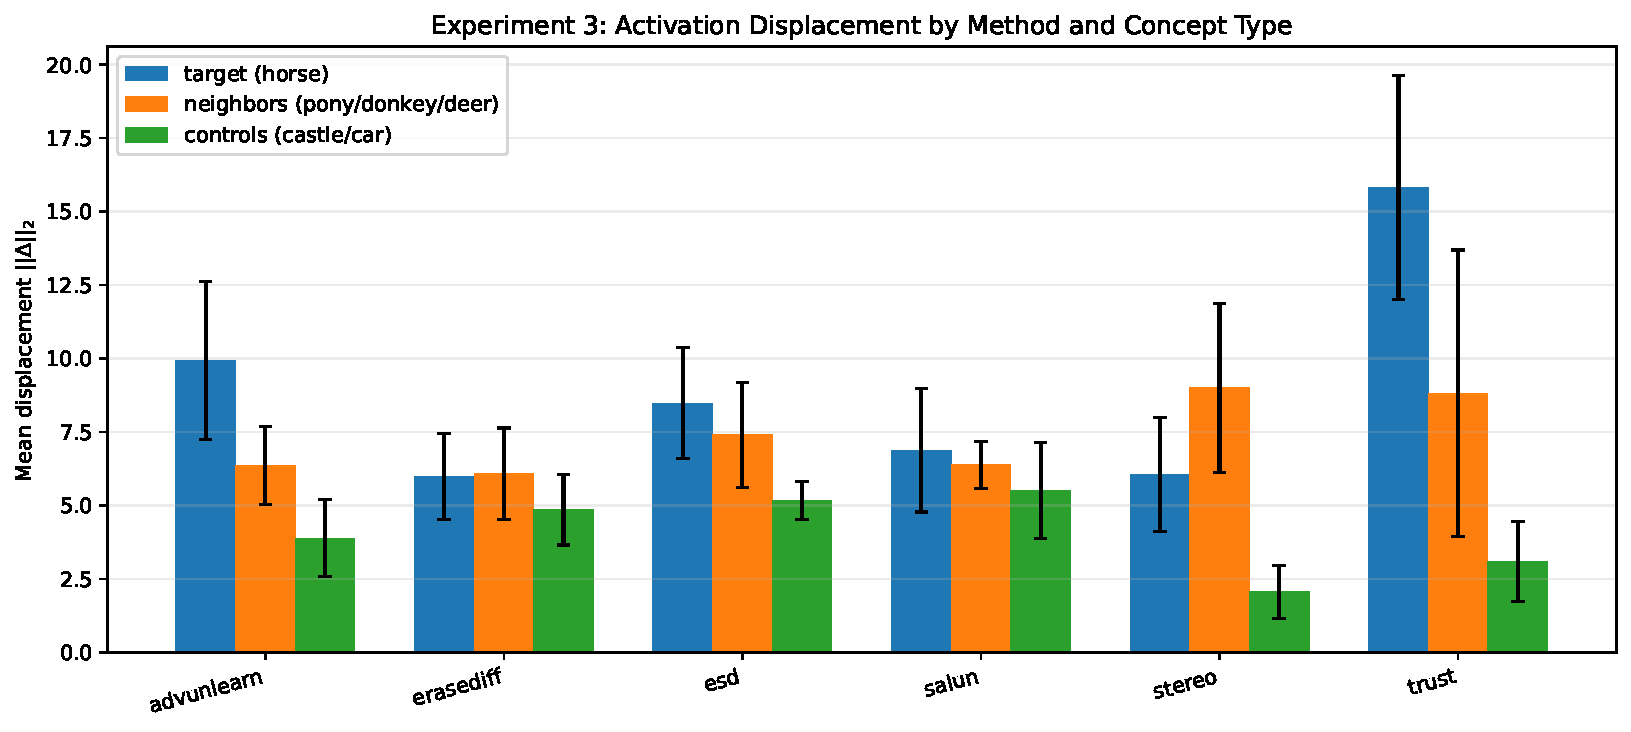
\includegraphics[width=0.8\linewidth]{img/fig_displacement_by_method_trust.pdf}
    \caption{
Mean activation displacement $\|\boldsymbol{\Phi}_{\hat\theta}(p) - \boldsymbol{\Phi}_\theta(p)\|_2$ for six unlearning methods erasing \texttt{horse}. Target prompts (blue) confirm~\cref{asm:edit}: erasure requires measurable displacement. Neighbor prompts (orange) are displaced more than control prompts (green) for all methods, consistent with the propagation mechanism in~\cref{thm:tradeoff}.
}
    \label{fig:placeholder}
\end{figure}
\newpage
\section{New Concepts}
\begin{table*}[htbp]
\centering
\caption{Results for the five additional target concepts. Original denotes the pretrained model before unlearning. All evaluation metrics are percentages. Higher UA, IRA, NP, and CP are better; lower IRR and DamageGap are better. DamageGap is the difference between control preservation (CP) and neighbor preservation (NP).}
\label{tab:new_concept_results}
\resizebox{\textwidth}{!}{
\begin{tabular}{llccccccc}
\toprule
Concept & Method & $\hat{\kappa}$ & UA (\%) $\uparrow$ & IRR (\%) $\downarrow$ & IRA (\%) $\uparrow$ & NP (\%) $\uparrow$ & CP (\%) $\uparrow$ & DamageGap (\%) $\downarrow$ \\
\midrule
Snake
& Original  & 0.37 & 9.2 & 6.0 & 31.1 & 100.0 & 100.0 & 0.0 \\
& EraseDiff & 0.37 & 88.1 & 8.6 & 19.1 & 81.2 & 93.6 & 12.4 \\
& ESD       & 0.37 & 97.9 & 6.8 & 20.6 & 81.3 & 98.1 & 16.8 \\
& SalUn     & 0.37 & 100.0 & 0.0 & 5.5 & 72.4 & 86.2 & 13.8 \\
& STEREO    & 0.37 & 100.0 & 0.0 & 14.8 & 25.1 & 96.0 & 71.1 \\
\midrule
Fish
& Original  & 0.52 & 6.2 & 11.0 & 40.5 & 100.0 & 100.0 & 0.0 \\
& EraseDiff & 0.52 & 92.3 & 5.3 & 23.2 & 78.0 & 92.1 & 14.1 \\
& ESD       & 0.52 & 94.5 & 2.7 & 34.5 & 79.2 & 98.0 & 18.8 \\
& SalUn     & 0.52 & 100.0 & 0.0 & 14.9 & 67.5 & 97.8 & 30.3 \\
& STEREO    & 0.52 & 100.0 & 0.0 & 5.8 & 23.2 & 38.4 & 15.2 \\
\midrule
Tree
& Original  & 0.63 & 4.4 & 61.8 & 51.8 & 100.0 & 100.0 & 0.0 \\
& EraseDiff & 0.63 & 32.0 & 55.2 & 53.8 & 75.1 & 98.0 & 22.9 \\
& ESD       & 0.63 & 39.7 & 48.0 & 50.3 & 82.4 & 98.9 & 16.5 \\
& SalUn     & 0.63 & 100.0 & 0.0 & 5.8 & 62.7 & 88.0 & 25.3 \\
& STEREO    & 0.63 & 100.0 & 0.0 & 4.9 & 26.6 & 32.0 & 5.4 \\
\midrule
Butterfly
& Original  & 0.66 & 7.1 & 12.2 & 36.0 & 100.0 & 100.0 & 0.0 \\
& EraseDiff & 0.66 & 46.2 & 37.3 & 34.6 & 74.7 & 92.5 & 17.8 \\
& ESD       & 0.66 & 72.6 & 28.9 & 31.2 & 78.1 & 83.3 & 5.2 \\
& SalUn     & 0.66 & 100.0 & 0.0 & 0.9 & 73.1 & 93.9 & 20.8 \\
& STEREO    & 0.66 & 100.0 & 0.0 & 10.5 & 19.2 & 68.0 & 48.8 \\
\midrule
Car
& Original  & 0.83 & 2.6 & 60.0 & 87.5 & 100.0 & 100.0 & 0.0 \\
& EraseDiff & 0.83 & 47.4 & 49.3 & 69.2 & 78.7 & 91.2 & 12.4 \\
& ESD       & 0.83 & 60.5 & 28.6 & 75.8 & 73.8 & 98.6 & 24.8 \\
& SalUn     & 0.83 & 79.3 & 16.1 & 17.8 & 66.8 & 85.6 & 18.8 \\
& STEREO    & 0.83 & 99.1 & 4.3 & 21.1 & 16.0 & 75.2 & 59.1 \\
\bottomrule
\end{tabular}
}
\end{table*}
\newpage
\section{Pareto with dashed lines}
\begin{figure}[htbp]
    \centering
    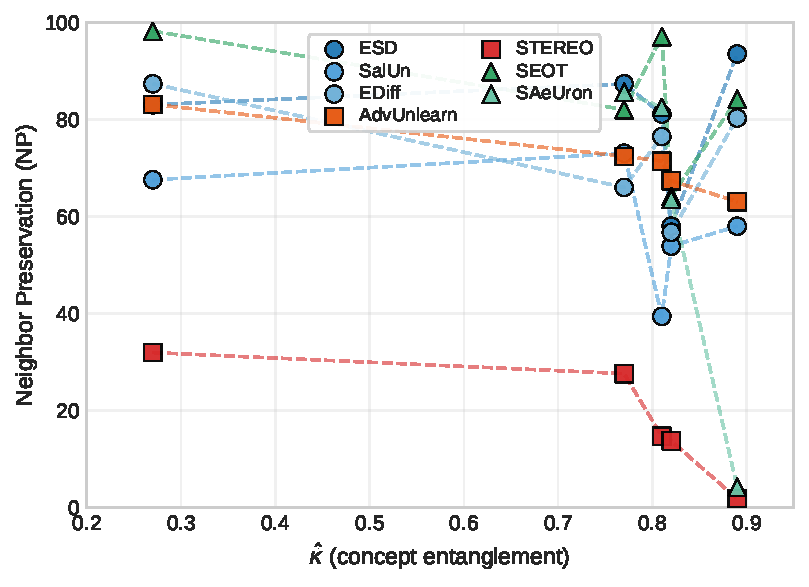
\includegraphics[width=0.5\linewidth]{img/kappa_np_scaling_dashed.pdf}
    \caption{NP across concept entanglement levels for each unlearning method. Dashed lines connect concept-specific operating points from the same method in increasing order of $\hat{\kappa}$ and are included as visual guides rather than fitted trends. Robust methods such as STEREO show a pronounced decline in NP as entanglement increases, while other methods exhibit weaker or more concept-dependent trends.}
    \label{fig:Pareto_dashed}
\end{figure}
\newpage


\end{document}
